\pdfoutput=1
\documentclass[10pt,a4paper]{article}
\usepackage[T1]{fontenc}
\usepackage[utf8]{inputenc}
\usepackage{lmodern}
\usepackage{microtype}
\usepackage[margin=2.5cm]{geometry}
\usepackage{amsmath,amssymb,amsthm}
\usepackage{booktabs}
\usepackage{array}
\usepackage{graphicx}
\usepackage{xcolor}
\usepackage[numbers,sort&compress]{natbib}
\usepackage{caption}
\usepackage{enumitem}
\usepackage{placeins}
\usepackage[hidelinks]{hyperref}
\captionsetup{font=small,labelfont=bf}
\setlist{itemsep=2pt,topsep=3pt}
\graphicspath{{figures/}}

% generated; do not edit
\expandafter\def\csname v@H1a.distinct\endcsname{2}
\expandafter\def\csname v@H1a.n\endcsname{4}
\expandafter\def\csname v@H1a.sig\endcsname{4}
\expandafter\def\csname v@H1a.verdict\endcsname{supported}
\expandafter\def\csname v@H1b.n\endcsname{4}
\expandafter\def\csname v@H1b.sig\endcsname{4}
\expandafter\def\csname v@H1b.sp.hi\endcsname{-0.428}
\expandafter\def\csname v@H1b.sp.k2\endcsname{0.435}
\expandafter\def\csname v@H1b.sp.k32\endcsname{0.007}
\expandafter\def\csname v@H1b.sp.lo\endcsname{-0.429}
\expandafter\def\csname v@H1b.verdict\endcsname{supported}
\expandafter\def\csname v@H1c.CONTRAST/pair\endcsname{0.52}
\expandafter\def\csname v@H1c.CONTRAST/triple\endcsname{0.48}
\expandafter\def\csname v@H1c.SUM/pair\endcsname{0.55}
\expandafter\def\csname v@H1c.SUM/triple\endcsname{1.00}
\expandafter\def\csname v@H1c.cells\endcsname{4}
\expandafter\def\csname v@H1c.cells.sup\endcsname{1}
\expandafter\def\csname v@H1c.verdict\endcsname{inconclusive}
\expandafter\def\csname v@H1c.verdict.CONTRAST/pair\endcsname{inconclusive}
\expandafter\def\csname v@H1c.verdict.CONTRAST/triple\endcsname{not supported}
\expandafter\def\csname v@H1c.verdict.SUM/pair\endcsname{inconclusive}
\expandafter\def\csname v@H1c.verdict.SUM/triple\endcsname{supported}
\expandafter\def\csname v@H2a.distinct\endcsname{10}
\expandafter\def\csname v@H2a.n\endcsname{20}
\expandafter\def\csname v@H2a.sig\endcsname{20}
\expandafter\def\csname v@H2a.verdict\endcsname{supported}
\expandafter\def\csname v@H2b_gauss.n\endcsname{8}
\expandafter\def\csname v@H2b_gauss.sig\endcsname{8}
\expandafter\def\csname v@H2b_gauss.verdict\endcsname{supported}
\expandafter\def\csname v@H2b_population.distinct\endcsname{4}
\expandafter\def\csname v@H2b_population.n\endcsname{8}
\expandafter\def\csname v@H2b_population.sig\endcsname{8}
\expandafter\def\csname v@H2b_population.verdict\endcsname{supported}
\expandafter\def\csname v@H2c.n\endcsname{221}
\expandafter\def\csname v@H2c.share\endcsname{60\,\%}
\expandafter\def\csname v@H2c.verdict\endcsname{inconclusive}
\expandafter\def\csname v@H3a.in\endcsname{21}
\expandafter\def\csname v@H3a.n\endcsname{48}
\expandafter\def\csname v@H3a.out\endcsname{27}
\expandafter\def\csname v@H3a.verdict\endcsname{not supported}
\expandafter\def\csname v@H3b.in\endcsname{73}
\expandafter\def\csname v@H3b.n\endcsname{236}
\expandafter\def\csname v@H3b.out\endcsname{156}
\expandafter\def\csname v@H3b.verdict\endcsname{not supported}
\expandafter\def\csname v@H3c.n\endcsname{272}
\expandafter\def\csname v@H3c.pair\endcsname{39\,\%}
\expandafter\def\csname v@H3c.triple\endcsname{34\,\%}
\expandafter\def\csname v@H3c.verdict\endcsname{not supported}
\expandafter\def\csname v@H4a.n\endcsname{114}
\expandafter\def\csname v@H4a.ratio\endcsname{2.1}
\expandafter\def\csname v@H4a.share\endcsname{93\,\%}
\expandafter\def\csname v@H4a.verdict\endcsname{supported}
\expandafter\def\csname v@H4b.k32\endcsname{4{,}962}
\expandafter\def\csname v@H4b.k8\endcsname{498}
\expandafter\def\csname v@H4b.maxchange\endcsname{8.3}
\expandafter\def\csname v@H4b.n2\endcsname{291{,}258}
\expandafter\def\csname v@H4b.n2share\endcsname{1.9\,\%}
\expandafter\def\csname v@H4b.other.viol\endcsname{0}
\expandafter\def\csname v@H4b.share\endcsname{0.47\,\%}
\expandafter\def\csname v@H4b.total\endcsname{1{,}165{,}059}
\expandafter\def\csname v@H4b.verdict\endcsname{not supported}
\expandafter\def\csname v@H4b.viol\endcsname{5{,}460}
\expandafter\def\csname v@H4b.worst.n2\endcsname{36.2}
\expandafter\def\csname v@H4b.worst.other\endcsname{0.86}
\expandafter\def\csname v@H5a.n\endcsname{72}
\expandafter\def\csname v@H5a.opp\endcsname{51}
\expandafter\def\csname v@H5a.ratio.S2\endcsname{0.05}
\expandafter\def\csname v@H5a.ratio.S3c\endcsname{0.06}
\expandafter\def\csname v@H5a.ratio.S4\endcsname{1.25}
\expandafter\def\csname v@H5a.sig\endcsname{11}
\expandafter\def\csname v@H5a.verdict\endcsname{not supported}
\expandafter\def\csname v@H5b.n\endcsname{18}
\expandafter\def\csname v@H5b.opp\endcsname{1}
\expandafter\def\csname v@H5b.sig\endcsname{5}
\expandafter\def\csname v@H5b.verdict\endcsname{not supported}
\expandafter\def\csname v@H5c.n\endcsname{78}
\expandafter\def\csname v@H5c.opp\endcsname{19}
\expandafter\def\csname v@H5c.sig\endcsname{24}
\expandafter\def\csname v@H5c.verdict\endcsname{not supported}
\expandafter\def\csname v@H5d.n\endcsname{192}
\expandafter\def\csname v@H5d.opp\endcsname{84}
\expandafter\def\csname v@H5d.sig\endcsname{27}
\expandafter\def\csname v@H5d.verdict\endcsname{not supported}
\expandafter\def\csname v@batches.n\endcsname{5}
\expandafter\def\csname v@bel.CONTRAST.16.S2.d1\endcsname{---}
\expandafter\def\csname v@bel.CONTRAST.16.S2.und\endcsname{0.075}
\expandafter\def\csname v@bel.CONTRAST.16.S3a.d1\endcsname{---}
\expandafter\def\csname v@bel.CONTRAST.16.S3a.und\endcsname{0.150}
\expandafter\def\csname v@bel.CONTRAST.16.S3b.d1\endcsname{---}
\expandafter\def\csname v@bel.CONTRAST.16.S3b.und\endcsname{0.900}
\expandafter\def\csname v@bel.CONTRAST.16.S3c.d1\endcsname{---}
\expandafter\def\csname v@bel.CONTRAST.16.S3c.und\endcsname{0.075}
\expandafter\def\csname v@bel.CONTRAST.16.S3d.d1\endcsname{---}
\expandafter\def\csname v@bel.CONTRAST.16.S3d.und\endcsname{---}
\expandafter\def\csname v@bel.CONTRAST.16.S4.d1\endcsname{---}
\expandafter\def\csname v@bel.CONTRAST.16.S4.und\endcsname{0.075}
\expandafter\def\csname v@bel.CONTRAST.2.S2.d1\endcsname{0.192}
\expandafter\def\csname v@bel.CONTRAST.2.S2.und\endcsname{0.450}
\expandafter\def\csname v@bel.CONTRAST.2.S3a.d1\endcsname{---}
\expandafter\def\csname v@bel.CONTRAST.2.S3a.und\endcsname{0.450}
\expandafter\def\csname v@bel.CONTRAST.2.S3b.d1\endcsname{---}
\expandafter\def\csname v@bel.CONTRAST.2.S3b.und\endcsname{0.450}
\expandafter\def\csname v@bel.CONTRAST.2.S3c.d1\endcsname{0.102}
\expandafter\def\csname v@bel.CONTRAST.2.S3c.und\endcsname{0.450}
\expandafter\def\csname v@bel.CONTRAST.2.S3d.d1\endcsname{---}
\expandafter\def\csname v@bel.CONTRAST.2.S3d.und\endcsname{0.600}
\expandafter\def\csname v@bel.CONTRAST.2.S4.d1\endcsname{---}
\expandafter\def\csname v@bel.CONTRAST.2.S4.und\endcsname{0.450}
\expandafter\def\csname v@bel.CONTRAST.32.S2.d1\endcsname{---}
\expandafter\def\csname v@bel.CONTRAST.32.S2.und\endcsname{0.010}
\expandafter\def\csname v@bel.CONTRAST.32.S3a.d1\endcsname{---}
\expandafter\def\csname v@bel.CONTRAST.32.S3a.und\endcsname{---}
\expandafter\def\csname v@bel.CONTRAST.32.S3b.d1\endcsname{---}
\expandafter\def\csname v@bel.CONTRAST.32.S3b.und\endcsname{---}
\expandafter\def\csname v@bel.CONTRAST.32.S3c.d1\endcsname{---}
\expandafter\def\csname v@bel.CONTRAST.32.S3c.und\endcsname{0.050}
\expandafter\def\csname v@bel.CONTRAST.32.S3d.d1\endcsname{---}
\expandafter\def\csname v@bel.CONTRAST.32.S3d.und\endcsname{---}
\expandafter\def\csname v@bel.CONTRAST.32.S4.d1\endcsname{---}
\expandafter\def\csname v@bel.CONTRAST.32.S4.und\endcsname{0.010}
\expandafter\def\csname v@bel.CONTRAST.4.S2.d1\endcsname{0.122}
\expandafter\def\csname v@bel.CONTRAST.4.S2.und\endcsname{0.200}
\expandafter\def\csname v@bel.CONTRAST.4.S3a.d1\endcsname{---}
\expandafter\def\csname v@bel.CONTRAST.4.S3a.und\endcsname{0.250}
\expandafter\def\csname v@bel.CONTRAST.4.S3b.d1\endcsname{---}
\expandafter\def\csname v@bel.CONTRAST.4.S3b.und\endcsname{0.250}
\expandafter\def\csname v@bel.CONTRAST.4.S3c.d1\endcsname{0.177}
\expandafter\def\csname v@bel.CONTRAST.4.S3c.und\endcsname{0.250}
\expandafter\def\csname v@bel.CONTRAST.4.S3d.d1\endcsname{---}
\expandafter\def\csname v@bel.CONTRAST.4.S3d.und\endcsname{0.350}
\expandafter\def\csname v@bel.CONTRAST.4.S4.d1\endcsname{---}
\expandafter\def\csname v@bel.CONTRAST.4.S4.und\endcsname{0.200}
\expandafter\def\csname v@bel.CONTRAST.8.S2.d1\endcsname{0.084}
\expandafter\def\csname v@bel.CONTRAST.8.S2.und\endcsname{0.150}
\expandafter\def\csname v@bel.CONTRAST.8.S3a.d1\endcsname{---}
\expandafter\def\csname v@bel.CONTRAST.8.S3a.und\endcsname{0.150}
\expandafter\def\csname v@bel.CONTRAST.8.S3b.d1\endcsname{---}
\expandafter\def\csname v@bel.CONTRAST.8.S3b.und\endcsname{0.200}
\expandafter\def\csname v@bel.CONTRAST.8.S3c.d1\endcsname{---}
\expandafter\def\csname v@bel.CONTRAST.8.S3c.und\endcsname{0.150}
\expandafter\def\csname v@bel.CONTRAST.8.S3d.d1\endcsname{---}
\expandafter\def\csname v@bel.CONTRAST.8.S3d.und\endcsname{0.350}
\expandafter\def\csname v@bel.CONTRAST.8.S4.d1\endcsname{---}
\expandafter\def\csname v@bel.CONTRAST.8.S4.und\endcsname{0.150}
\expandafter\def\csname v@bel.SUM.16.S2.d1\endcsname{0.043}
\expandafter\def\csname v@bel.SUM.16.S2.und\endcsname{0.075}
\expandafter\def\csname v@bel.SUM.16.S3a.d1\endcsname{---}
\expandafter\def\csname v@bel.SUM.16.S3a.und\endcsname{0.150}
\expandafter\def\csname v@bel.SUM.16.S3b.d1\endcsname{0.009}
\expandafter\def\csname v@bel.SUM.16.S3b.und\endcsname{0.900}
\expandafter\def\csname v@bel.SUM.16.S3c.d1\endcsname{---}
\expandafter\def\csname v@bel.SUM.16.S3c.und\endcsname{0.075}
\expandafter\def\csname v@bel.SUM.16.S3d.d1\endcsname{---}
\expandafter\def\csname v@bel.SUM.16.S3d.und\endcsname{---}
\expandafter\def\csname v@bel.SUM.16.S4.d1\endcsname{---}
\expandafter\def\csname v@bel.SUM.16.S4.und\endcsname{0.075}
\expandafter\def\csname v@bel.SUM.2.S2.d1\endcsname{0.192}
\expandafter\def\csname v@bel.SUM.2.S2.und\endcsname{0.450}
\expandafter\def\csname v@bel.SUM.2.S3a.d1\endcsname{---}
\expandafter\def\csname v@bel.SUM.2.S3a.und\endcsname{0.450}
\expandafter\def\csname v@bel.SUM.2.S3b.d1\endcsname{---}
\expandafter\def\csname v@bel.SUM.2.S3b.und\endcsname{0.450}
\expandafter\def\csname v@bel.SUM.2.S3c.d1\endcsname{0.217}
\expandafter\def\csname v@bel.SUM.2.S3c.und\endcsname{0.450}
\expandafter\def\csname v@bel.SUM.2.S3d.d1\endcsname{---}
\expandafter\def\csname v@bel.SUM.2.S3d.und\endcsname{0.600}
\expandafter\def\csname v@bel.SUM.2.S4.d1\endcsname{---}
\expandafter\def\csname v@bel.SUM.2.S4.und\endcsname{0.450}
\expandafter\def\csname v@bel.SUM.32.S2.d1\endcsname{---}
\expandafter\def\csname v@bel.SUM.32.S2.und\endcsname{0.010}
\expandafter\def\csname v@bel.SUM.32.S3a.d1\endcsname{0.054}
\expandafter\def\csname v@bel.SUM.32.S3a.und\endcsname{---}
\expandafter\def\csname v@bel.SUM.32.S3b.d1\endcsname{0.027}
\expandafter\def\csname v@bel.SUM.32.S3b.und\endcsname{---}
\expandafter\def\csname v@bel.SUM.32.S3c.d1\endcsname{---}
\expandafter\def\csname v@bel.SUM.32.S3c.und\endcsname{0.050}
\expandafter\def\csname v@bel.SUM.32.S3d.d1\endcsname{---}
\expandafter\def\csname v@bel.SUM.32.S3d.und\endcsname{---}
\expandafter\def\csname v@bel.SUM.32.S4.d1\endcsname{---}
\expandafter\def\csname v@bel.SUM.32.S4.und\endcsname{0.010}
\expandafter\def\csname v@bel.SUM.4.S2.d1\endcsname{0.102}
\expandafter\def\csname v@bel.SUM.4.S2.und\endcsname{0.200}
\expandafter\def\csname v@bel.SUM.4.S3a.d1\endcsname{---}
\expandafter\def\csname v@bel.SUM.4.S3a.und\endcsname{0.250}
\expandafter\def\csname v@bel.SUM.4.S3b.d1\endcsname{0.039}
\expandafter\def\csname v@bel.SUM.4.S3b.und\endcsname{0.250}
\expandafter\def\csname v@bel.SUM.4.S3c.d1\endcsname{0.125}
\expandafter\def\csname v@bel.SUM.4.S3c.und\endcsname{0.200}
\expandafter\def\csname v@bel.SUM.4.S3d.d1\endcsname{---}
\expandafter\def\csname v@bel.SUM.4.S3d.und\endcsname{0.350}
\expandafter\def\csname v@bel.SUM.4.S4.d1\endcsname{---}
\expandafter\def\csname v@bel.SUM.4.S4.und\endcsname{0.200}
\expandafter\def\csname v@bel.SUM.8.S2.d1\endcsname{0.067}
\expandafter\def\csname v@bel.SUM.8.S2.und\endcsname{0.150}
\expandafter\def\csname v@bel.SUM.8.S3a.d1\endcsname{---}
\expandafter\def\csname v@bel.SUM.8.S3a.und\endcsname{0.150}
\expandafter\def\csname v@bel.SUM.8.S3b.d1\endcsname{0.014}
\expandafter\def\csname v@bel.SUM.8.S3b.und\endcsname{0.200}
\expandafter\def\csname v@bel.SUM.8.S3c.d1\endcsname{---}
\expandafter\def\csname v@bel.SUM.8.S3c.und\endcsname{0.150}
\expandafter\def\csname v@bel.SUM.8.S3d.d1\endcsname{---}
\expandafter\def\csname v@bel.SUM.8.S3d.und\endcsname{0.350}
\expandafter\def\csname v@bel.SUM.8.S4.d1\endcsname{---}
\expandafter\def\csname v@bel.SUM.8.S4.und\endcsname{0.150}
\expandafter\def\csname v@cfg.M\endcsname{2^{20}}
\expandafter\def\csname v@cfg.R\endcsname{16}
\expandafter\def\csname v@cfg.a\endcsname{0.6}
\expandafter\def\csname v@cfg.b\endcsname{0.5}
\expandafter\def\csname v@cfg.floor\endcsname{0.01}
\expandafter\def\csname v@cfg.gl\endcsname{192}
\expandafter\def\csname v@cfg.snodes\endcsname{801}
\expandafter\def\csname v@cfg.starts\endcsname{2{,}000}
\expandafter\def\csname v@clip.S4.ec\endcsname{0.024}
\expandafter\def\csname v@clip.S4.eu\endcsname{0.0004}
\expandafter\def\csname v@clip.dneg.0.001\endcsname{0.024}
\expandafter\def\csname v@clip.dneg.0.01\endcsname{0.025}
\expandafter\def\csname v@clip.dneg.0.1\endcsname{0.028}
\expandafter\def\csname v@clip.max\endcsname{39\,\%}
\expandafter\def\csname v@clip.min\endcsname{0\,\%}
\expandafter\def\csname v@coef.pair\endcsname{8{,}581}
\expandafter\def\csname v@coef.triple\endcsname{357{,}765}
\expandafter\def\csname v@cor.err\endcsname{\ensuremath{4\times 10^{-10}}}
\expandafter\def\csname v@cor.min\endcsname{0.32}
\expandafter\def\csname v@cut.drop\endcsname{\ensuremath{3\times 10^{-4}}}
\expandafter\def\csname v@cut.in.hi\endcsname{0.79}
\expandafter\def\csname v@cut.in.lo\endcsname{0.52}
\expandafter\def\csname v@cut.sign.2\endcsname{14\,\%}
\expandafter\def\csname v@cut.sign.32\endcsname{100\,\%}
\expandafter\def\csname v@d.rho02.k2\endcsname{0.011}
\expandafter\def\csname v@d3.closer\endcsname{32\,\%}
\expandafter\def\csname v@d3.closer.n\endcsname{145}
\expandafter\def\csname v@d3.flat.con\endcsname{0.041}
\expandafter\def\csname v@d3.flat.sum\endcsname{0.020}
\expandafter\def\csname v@d3.narrow.con\endcsname{0.0039}
\expandafter\def\csname v@d3.narrow.sum\endcsname{0.0005}
\expandafter\def\csname v@d3.taylor.r1k0\endcsname{0.0116}
\expandafter\def\csname v@d3.taylor.r1k1\endcsname{0.0022}
\expandafter\def\csname v@d3.taylor.r1k2\endcsname{0.0009}
\expandafter\def\csname v@d3.taylor.r4k0\endcsname{0.0353}
\expandafter\def\csname v@d3.taylor.r4k1\endcsname{0.0412}
\expandafter\def\csname v@d3.taylor.r4k2\endcsname{0.0758}
\expandafter\def\csname v@db.hi\endcsname{1.01}
\expandafter\def\csname v@db.lo\endcsname{0.97}
\expandafter\def\csname v@db.n\endcsname{85}
\expandafter\def\csname v@dec.S2.CONTRAST.0.1.d_denom\endcsname{0.0025}
\expandafter\def\csname v@dec.S2.CONTRAST.0.1.d_model_cal\endcsname{0.0026}
\expandafter\def\csname v@dec.S2.CONTRAST.0.1.d_model_uncal\endcsname{0.0129}
\expandafter\def\csname v@dec.S2.CONTRAST.0.1.d_neg\endcsname{0.0123}
\expandafter\def\csname v@dec.S2.CONTRAST.0.1.d_total\endcsname{0.0154}
\expandafter\def\csname v@dec.S2.CONTRAST.0.2.d_denom\endcsname{0.0108}
\expandafter\def\csname v@dec.S2.CONTRAST.0.2.d_model_cal\endcsname{0.0195}
\expandafter\def\csname v@dec.S2.CONTRAST.0.2.d_model_uncal\endcsname{0.0267}
\expandafter\def\csname v@dec.S2.CONTRAST.0.2.d_neg\endcsname{0.0095}
\expandafter\def\csname v@dec.S2.CONTRAST.0.2.d_total\endcsname{0.0374}
\expandafter\def\csname v@dec.S2.CONTRAST.0.4.d_denom\endcsname{0.0547}
\expandafter\def\csname v@dec.S2.CONTRAST.0.4.d_model_cal\endcsname{0.0617}
\expandafter\def\csname v@dec.S2.CONTRAST.0.4.d_model_uncal\endcsname{0.0397}
\expandafter\def\csname v@dec.S2.CONTRAST.0.4.d_neg\endcsname{0.0238}
\expandafter\def\csname v@dec.S2.CONTRAST.0.4.d_total\endcsname{0.0906}
\expandafter\def\csname v@dec.S2.SUM.0.1.d_denom\endcsname{0.0025}
\expandafter\def\csname v@dec.S2.SUM.0.1.d_model_cal\endcsname{0.0241}
\expandafter\def\csname v@dec.S2.SUM.0.1.d_model_uncal\endcsname{0.0131}
\expandafter\def\csname v@dec.S2.SUM.0.1.d_neg\endcsname{0.0111}
\expandafter\def\csname v@dec.S2.SUM.0.1.d_total\endcsname{0.0106}
\expandafter\def\csname v@dec.S2.SUM.0.2.d_denom\endcsname{0.0108}
\expandafter\def\csname v@dec.S2.SUM.0.2.d_model_cal\endcsname{0.0358}
\expandafter\def\csname v@dec.S2.SUM.0.2.d_model_uncal\endcsname{0.0287}
\expandafter\def\csname v@dec.S2.SUM.0.2.d_neg\endcsname{0.0076}
\expandafter\def\csname v@dec.S2.SUM.0.2.d_total\endcsname{0.0180}
\expandafter\def\csname v@dec.S2.SUM.0.4.d_denom\endcsname{0.0736}
\expandafter\def\csname v@dec.S2.SUM.0.4.d_model_cal\endcsname{0.0627}
\expandafter\def\csname v@dec.S2.SUM.0.4.d_model_uncal\endcsname{0.1002}
\expandafter\def\csname v@dec.S2.SUM.0.4.d_neg\endcsname{0.0376}
\expandafter\def\csname v@dec.S2.SUM.0.4.d_total\endcsname{0.0265}
\expandafter\def\csname v@dec.S3c.CONTRAST.0.1.d_denom\endcsname{0.0097}
\expandafter\def\csname v@dec.S3c.CONTRAST.0.1.d_model_cal\endcsname{0.0673}
\expandafter\def\csname v@dec.S3c.CONTRAST.0.1.d_model_uncal\endcsname{0.0650}
\expandafter\def\csname v@dec.S3c.CONTRAST.0.1.d_neg\endcsname{0.0391}
\expandafter\def\csname v@dec.S3c.CONTRAST.0.1.d_total\endcsname{0.0710}
\expandafter\def\csname v@dec.S3c.CONTRAST.0.2.d_denom\endcsname{0.0262}
\expandafter\def\csname v@dec.S3c.CONTRAST.0.2.d_model_cal\endcsname{0.0971}
\expandafter\def\csname v@dec.S3c.CONTRAST.0.2.d_model_uncal\endcsname{0.0854}
\expandafter\def\csname v@dec.S3c.CONTRAST.0.2.d_neg\endcsname{0.0551}
\expandafter\def\csname v@dec.S3c.CONTRAST.0.2.d_total\endcsname{0.1022}
\expandafter\def\csname v@dec.S3c.CONTRAST.0.4.d_denom\endcsname{0.1030}
\expandafter\def\csname v@dec.S3c.CONTRAST.0.4.d_model_cal\endcsname{0.1371}
\expandafter\def\csname v@dec.S3c.CONTRAST.0.4.d_model_uncal\endcsname{0.0985}
\expandafter\def\csname v@dec.S3c.CONTRAST.0.4.d_neg\endcsname{0.1116}
\expandafter\def\csname v@dec.S3c.CONTRAST.0.4.d_total\endcsname{0.1526}
\expandafter\def\csname v@dec.S3c.SUM.0.1.d_denom\endcsname{0.0034}
\expandafter\def\csname v@dec.S3c.SUM.0.1.d_model_cal\endcsname{0.0445}
\expandafter\def\csname v@dec.S3c.SUM.0.1.d_model_uncal\endcsname{0.0399}
\expandafter\def\csname v@dec.S3c.SUM.0.1.d_neg\endcsname{0.0064}
\expandafter\def\csname v@dec.S3c.SUM.0.1.d_total\endcsname{0.0368}
\expandafter\def\csname v@dec.S3c.SUM.0.2.d_denom\endcsname{0.0087}
\expandafter\def\csname v@dec.S3c.SUM.0.2.d_model_cal\endcsname{0.0415}
\expandafter\def\csname v@dec.S3c.SUM.0.2.d_model_uncal\endcsname{0.0372}
\expandafter\def\csname v@dec.S3c.SUM.0.2.d_neg\endcsname{0.0064}
\expandafter\def\csname v@dec.S3c.SUM.0.2.d_total\endcsname{0.0294}
\expandafter\def\csname v@dec.S3c.SUM.0.4.d_denom\endcsname{0.0355}
\expandafter\def\csname v@dec.S3c.SUM.0.4.d_model_cal\endcsname{0.0438}
\expandafter\def\csname v@dec.S3c.SUM.0.4.d_model_uncal\endcsname{0.0485}
\expandafter\def\csname v@dec.S3c.SUM.0.4.d_neg\endcsname{0.0061}
\expandafter\def\csname v@dec.S3c.SUM.0.4.d_total\endcsname{0.0171}
\expandafter\def\csname v@dec.S4.CONTRAST.0.1.d_denom\endcsname{0.0001}
\expandafter\def\csname v@dec.S4.CONTRAST.0.1.d_model_cal\endcsname{0.0118}
\expandafter\def\csname v@dec.S4.CONTRAST.0.1.d_model_uncal\endcsname{0.0003}
\expandafter\def\csname v@dec.S4.CONTRAST.0.1.d_neg\endcsname{0.0118}
\expandafter\def\csname v@dec.S4.CONTRAST.0.1.d_total\endcsname{0.0003}
\expandafter\def\csname v@dec.S4.CONTRAST.0.2.d_denom\endcsname{0.0004}
\expandafter\def\csname v@dec.S4.CONTRAST.0.2.d_model_cal\endcsname{0.0101}
\expandafter\def\csname v@dec.S4.CONTRAST.0.2.d_model_uncal\endcsname{0.0004}
\expandafter\def\csname v@dec.S4.CONTRAST.0.2.d_neg\endcsname{0.0104}
\expandafter\def\csname v@dec.S4.CONTRAST.0.2.d_total\endcsname{0.0003}
\expandafter\def\csname v@dec.S4.CONTRAST.0.4.d_denom\endcsname{0.0003}
\expandafter\def\csname v@dec.S4.CONTRAST.0.4.d_model_cal\endcsname{0.0045}
\expandafter\def\csname v@dec.S4.CONTRAST.0.4.d_model_uncal\endcsname{0.0004}
\expandafter\def\csname v@dec.S4.CONTRAST.0.4.d_neg\endcsname{0.0044}
\expandafter\def\csname v@dec.S4.CONTRAST.0.4.d_total\endcsname{0.0004}
\expandafter\def\csname v@dec.S4.SUM.0.1.d_denom\endcsname{0.0001}
\expandafter\def\csname v@dec.S4.SUM.0.1.d_model_cal\endcsname{0.0119}
\expandafter\def\csname v@dec.S4.SUM.0.1.d_model_uncal\endcsname{0.0003}
\expandafter\def\csname v@dec.S4.SUM.0.1.d_neg\endcsname{0.0120}
\expandafter\def\csname v@dec.S4.SUM.0.1.d_total\endcsname{0.0003}
\expandafter\def\csname v@dec.S4.SUM.0.2.d_denom\endcsname{0.0004}
\expandafter\def\csname v@dec.S4.SUM.0.2.d_model_cal\endcsname{0.0100}
\expandafter\def\csname v@dec.S4.SUM.0.2.d_model_uncal\endcsname{0.0004}
\expandafter\def\csname v@dec.S4.SUM.0.2.d_neg\endcsname{0.0103}
\expandafter\def\csname v@dec.S4.SUM.0.2.d_total\endcsname{0.0003}
\expandafter\def\csname v@dec.S4.SUM.0.4.d_denom\endcsname{0.0003}
\expandafter\def\csname v@dec.S4.SUM.0.4.d_model_cal\endcsname{0.0037}
\expandafter\def\csname v@dec.S4.SUM.0.4.d_model_uncal\endcsname{0.0004}
\expandafter\def\csname v@dec.S4.SUM.0.4.d_neg\endcsname{0.0037}
\expandafter\def\csname v@dec.S4.SUM.0.4.d_total\endcsname{0.0002}
\expandafter\def\csname v@e2e.L4\endcsname{\ensuremath{2.4\times 10^{-4}}}
\expandafter\def\csname v@e2e.coef.hi\endcsname{6{,}364}
\expandafter\def\csname v@e2e.coef.lo\endcsname{61}
\expandafter\def\csname v@e2e.noise\endcsname{\ensuremath{1.8\times 10^{-4}}}
\expandafter\def\csname v@e2e.targets\endcsname{12}
\expandafter\def\csname v@en.HCR-CAL.32.J\endcsname{88.7}
\expandafter\def\csname v@en.HCR-CAL.32.ms\endcsname{308}
\expandafter\def\csname v@en.HCR-CAL.64.J\endcsname{168}
\expandafter\def\csname v@en.HCR-CAL.64.ms\endcsname{580}
\expandafter\def\csname v@en.HCR-CD.32.J\endcsname{0.137}
\expandafter\def\csname v@en.HCR-CD.32.ms\endcsname{0.484}
\expandafter\def\csname v@en.HCR-CD.64.J\endcsname{0.203}
\expandafter\def\csname v@en.HCR-CD.64.ms\endcsname{0.666}
\expandafter\def\csname v@en.KAN.32.J\endcsname{0.482}
\expandafter\def\csname v@en.KAN.32.ms\endcsname{1.91}
\expandafter\def\csname v@en.KAN.64.J\endcsname{0.829}
\expandafter\def\csname v@en.KAN.64.ms\endcsname{3.32}
\expandafter\def\csname v@en.MLP.32.J\endcsname{0.0682}
\expandafter\def\csname v@en.MLP.32.ms\endcsname{0.289}
\expandafter\def\csname v@en.MLP.64.J\endcsname{0.105}
\expandafter\def\csname v@en.MLP.64.ms\endcsname{0.297}
\expandafter\def\csname v@en.cal.over.cd.32\endcsname{647}
\expandafter\def\csname v@en.cal.over.cd.64\endcsname{828}
\expandafter\def\csname v@en.cd.over.mlp.32\endcsname{2.0}
\expandafter\def\csname v@en.cd.over.mlp.64\endcsname{1.9}
\expandafter\def\csname v@en.counter.hi\endcsname{1.061}
\expandafter\def\csname v@en.counter.lo\endcsname{0.953}
\expandafter\def\csname v@en.counter.med\endcsname{0.999}
\expandafter\def\csname v@en.idle.n\endcsname{8}
\expandafter\def\csname v@en.idle.of\endcsname{48}
\expandafter\def\csname v@en.kan.over.cd.32\endcsname{3.5}
\expandafter\def\csname v@en.kan.over.cd.64\endcsname{4.1}
\expandafter\def\csname v@en.limit.repeats\endcsname{71}
\expandafter\def\csname v@en.mlp.limit.W\endcsname{398}
\expandafter\def\csname v@en.mlpfast.32\endcsname{0.145}
\expandafter\def\csname v@en.mlpfast.64\endcsname{0.0667}
\expandafter\def\csname v@en.rel.hi1\endcsname{5}
\expandafter\def\csname v@en.rel.hi2\endcsname{6}
\expandafter\def\csname v@en.repeats\endcsname{4{,}320}
\expandafter\def\csname v@en.row.repeats\endcsname{90}
\expandafter\def\csname v@en.runs\endcsname{6}
\expandafter\def\csname v@en.runs.dtype\endcsname{3}
\expandafter\def\csname v@eqd.n\endcsname{800}
\expandafter\def\csname v@eqd.rel\endcsname{0.5\,\%}
\expandafter\def\csname v@eqd.s3c\endcsname{0.77}
\expandafter\def\csname v@eqd.triple\endcsname{1175}
\expandafter\def\csname v@failed\endcsname{0}
\expandafter\def\csname v@fam.clayton.min\endcsname{$-$0.179}
\expandafter\def\csname v@fam.clayton.ratio\endcsname{5.34}
\expandafter\def\csname v@fam.gumbel.min\endcsname{$-$0.128}
\expandafter\def\csname v@fam.gumbel.ratio\endcsname{16.60}
\expandafter\def\csname v@fam.t10.min\endcsname{$-$0.102}
\expandafter\def\csname v@fam.t10.ratio\endcsname{2.08}
\expandafter\def\csname v@fam.t3.min\endcsname{$-$0.201}
\expandafter\def\csname v@fam.t3.ratio\endcsname{7.22}
\expandafter\def\csname v@floor.shift\endcsname{0.045}
\expandafter\def\csname v@gpuh.billed\endcsname{196.25}
\expandafter\def\csname v@gpuh.jobs\endcsname{176.7}
\expandafter\def\csname v@hyp.inc\endcsname{2}
\expandafter\def\csname v@hyp.not\endcsname{8}
\expandafter\def\csname v@hyp.rows\endcsname{16}
\expandafter\def\csname v@hyp.sup\endcsname{5}
\expandafter\def\csname v@hyp.total\endcsname{15}
\expandafter\def\csname v@jobs\endcsname{2{,}900}
\expandafter\def\csname v@lead.hi\endcsname{1.76}
\expandafter\def\csname v@lead.lo\endcsname{0.57}
\expandafter\def\csname v@lead.n\endcsname{112}
\expandafter\def\csname v@lead.small.hi\endcsname{1.21}
\expandafter\def\csname v@lead.small.lo\endcsname{0.72}
\expandafter\def\csname v@lead.small.n\endcsname{64}
\expandafter\def\csname v@lkj.defined.k4\endcsname{0}
\expandafter\def\csname v@lkj.defined.k8\endcsname{0}
\expandafter\def\csname v@narrow.pair4\endcsname{0.0032}
\expandafter\def\csname v@narrow.triple2\endcsname{0.0211}
\expandafter\def\csname v@narrow.triple4\endcsname{0.0124}
\expandafter\def\csname v@nz.bound.hi\endcsname{77\,\%}
\expandafter\def\csname v@nz.bound.lo\endcsname{75\,\%}
\expandafter\def\csname v@nz.need.pair32\endcsname{\ensuremath{8.6\times 10^{6}}}
\expandafter\def\csname v@nz.need.triple16\endcsname{\ensuremath{1.1\times 10^{8}}}
\expandafter\def\csname v@nz.pair32.corner\endcsname{4.4}
\expandafter\def\csname v@nz.pair32.cube\endcsname{5.5}
\expandafter\def\csname v@nz.pair32.meas\endcsname{4.4}
\expandafter\def\csname v@nz.ratio.hi\endcsname{0.82}
\expandafter\def\csname v@nz.ratio.lo\endcsname{0.73}
\expandafter\def\csname v@nz.var\endcsname{0.98}
\expandafter\def\csname v@on.arc.2\endcsname{0.0398}
\expandafter\def\csname v@on.arc.32\endcsname{0.0025}
\expandafter\def\csname v@on.atoms.k32\endcsname{0.18}
\expandafter\def\csname v@on.atoms.k32b\endcsname{0.82}
\expandafter\def\csname v@on.conv.kr.128\endcsname{1.319}
\expandafter\def\csname v@on.conv.kr.2048\endcsname{1.325}
\expandafter\def\csname v@on.conv.kr.32\endcsname{1.263}
\expandafter\def\csname v@on.conv.kr.512\endcsname{1.324}
\expandafter\def\csname v@on.conv.kr.8\endcsname{1.015}
\expandafter\def\csname v@on.gap\endcsname{4.4\,\%}
\expandafter\def\csname v@on.gap4\endcsname{1.9\,\%}
\expandafter\def\csname v@on.kr.pair.hi\endcsname{1.26}
\expandafter\def\csname v@on.kr.pair.lo\endcsname{0.82}
\expandafter\def\csname v@on.pair.16.lower\endcsname{0.073}
\expandafter\def\csname v@on.pair.16.meas\endcsname{0.074}
\expandafter\def\csname v@on.pair.2.lower\endcsname{0.289}
\expandafter\def\csname v@on.pair.2.meas\endcsname{0.437}
\expandafter\def\csname v@on.pair.32.lower\endcsname{0.039}
\expandafter\def\csname v@on.pair.32.meas\endcsname{0.039}
\expandafter\def\csname v@on.pair.4.lower\endcsname{0.201}
\expandafter\def\csname v@on.pair.4.meas\endcsname{0.204}
\expandafter\def\csname v@on.pair.8.lower\endcsname{0.127}
\expandafter\def\csname v@on.pair.8.meas\endcsname{0.129}
\expandafter\def\csname v@on.tri.gap\endcsname{6.1\,\%}
\expandafter\def\csname v@on.tri.grid.err\endcsname{\ensuremath{1\times 10^{-13}}}
\expandafter\def\csname v@on.tri.grid.n\endcsname{13}
\expandafter\def\csname v@orth.pair\endcsname{\ensuremath{2\times 10^{-17}}}
\expandafter\def\csname v@pairs32\endcsname{496}
\expandafter\def\csname v@past.dc.hi\endcsname{0.086}
\expandafter\def\csname v@past.dc.lo\endcsname{0.001}
\expandafter\def\csname v@past.pair.hi\endcsname{0.10}
\expandafter\def\csname v@past.pair.lo\endcsname{0.05}
\expandafter\def\csname v@ph.H4a.all.n\endcsname{293}
\expandafter\def\csname v@ph.H4a.all.share\endcsname{96\,\%}
\expandafter\def\csname v@ph.H5b.e2e.n\endcsname{8}
\expandafter\def\csname v@ph.H5b.e2e.opp\endcsname{0}
\expandafter\def\csname v@ph.H5b.e2e.sig\endcsname{0}
\expandafter\def\csname v@ph.H5b.nll.n\endcsname{6}
\expandafter\def\csname v@ph.H5b.nll.opp\endcsname{0}
\expandafter\def\csname v@ph.H5b.nll.sig\endcsname{4}
\expandafter\def\csname v@ph.H5b.val.n\endcsname{4}
\expandafter\def\csname v@ph.H5b.val.opp\endcsname{1}
\expandafter\def\csname v@ph.H5b.val.sig\endcsname{1}
\expandafter\def\csname v@ph.H5c.e2e.n\endcsname{26}
\expandafter\def\csname v@ph.H5c.e2e.opp\endcsname{7}
\expandafter\def\csname v@ph.H5c.e2e.sig\endcsname{0}
\expandafter\def\csname v@ph.H5c.nll.n\endcsname{26}
\expandafter\def\csname v@ph.H5c.nll.opp\endcsname{4}
\expandafter\def\csname v@ph.H5c.nll.sig\endcsname{21}
\expandafter\def\csname v@ph.H5c.val.n\endcsname{26}
\expandafter\def\csname v@ph.H5c.val.opp\endcsname{8}
\expandafter\def\csname v@ph.H5c.val.sig\endcsname{3}
\expandafter\def\csname v@ph.H5d.L.1.n\endcsname{48}
\expandafter\def\csname v@ph.H5d.L.1.opp\endcsname{32}
\expandafter\def\csname v@ph.H5d.L.1.sig\endcsname{7}
\expandafter\def\csname v@ph.H5d.L.2.n\endcsname{48}
\expandafter\def\csname v@ph.H5d.L.2.opp\endcsname{28}
\expandafter\def\csname v@ph.H5d.L.2.sig\endcsname{11}
\expandafter\def\csname v@ph.H5d.L.3.n\endcsname{48}
\expandafter\def\csname v@ph.H5d.L.3.opp\endcsname{20}
\expandafter\def\csname v@ph.H5d.L.3.sig\endcsname{6}
\expandafter\def\csname v@ph.H5d.L.4.n\endcsname{48}
\expandafter\def\csname v@ph.H5d.L.4.opp\endcsname{4}
\expandafter\def\csname v@ph.H5d.L.4.sig\endcsname{3}
\expandafter\def\csname v@ph.H5d.basis.pair.n\endcsname{96}
\expandafter\def\csname v@ph.H5d.basis.pair.opp\endcsname{53}
\expandafter\def\csname v@ph.H5d.basis.pair.sig\endcsname{4}
\expandafter\def\csname v@ph.H5d.basis.triple.n\endcsname{96}
\expandafter\def\csname v@ph.H5d.basis.triple.opp\endcsname{31}
\expandafter\def\csname v@ph.H5d.basis.triple.sig\endcsname{23}
\expandafter\def\csname v@ph.H5d.k.2.n\endcsname{64}
\expandafter\def\csname v@ph.H5d.k.2.opp\endcsname{30}
\expandafter\def\csname v@ph.H5d.k.2.sig\endcsname{0}
\expandafter\def\csname v@ph.H5d.k.4.n\endcsname{64}
\expandafter\def\csname v@ph.H5d.k.4.opp\endcsname{29}
\expandafter\def\csname v@ph.H5d.k.4.sig\endcsname{6}
\expandafter\def\csname v@ph.H5d.k.8.n\endcsname{64}
\expandafter\def\csname v@ph.H5d.k.8.opp\endcsname{25}
\expandafter\def\csname v@ph.H5d.k.8.sig\endcsname{21}
\expandafter\def\csname v@ph.a6\endcsname{0.047}
\expandafter\def\csname v@ph.bound.max\endcsname{0.86}
\expandafter\def\csname v@ph.bound.med\endcsname{0.037}
\expandafter\def\csname v@ph.bound.n\endcsname{149{,}880}
\expandafter\def\csname v@ph.chi.max\endcsname{1.05}
\expandafter\def\csname v@ph.chi.min\endcsname{1.04}
\expandafter\def\csname v@ph.closer.S2_pair\endcsname{71\,\%}
\expandafter\def\csname v@ph.closer.S2_triple\endcsname{42\,\%}
\expandafter\def\csname v@ph.closer.S3b_pair\endcsname{24\,\%}
\expandafter\def\csname v@ph.closer.S3c_pair\endcsname{71\,\%}
\expandafter\def\csname v@ph.closer.S4_pair\endcsname{98\,\%}
\expandafter\def\csname v@ph.closer.S4_triple\endcsname{50\,\%}
\expandafter\def\csname v@ph.closer.all\endcsname{57\,\%}
\expandafter\def\csname v@ph.closer.def\endcsname{60\,\%}
\expandafter\def\csname v@ph.closer.undef\endcsname{55\,\%}
\expandafter\def\csname v@ph.closer.undef.pair\endcsname{59\,\%}
\expandafter\def\csname v@ph.depth.S2.pair.1\endcsname{0.0648}
\expandafter\def\csname v@ph.depth.S2.pair.4\endcsname{0.0024}
\expandafter\def\csname v@ph.depth.S2.triple.1\endcsname{0.0653}
\expandafter\def\csname v@ph.depth.S2.triple.4\endcsname{0.0025}
\expandafter\def\csname v@ph.depth.S3c.pair.1\endcsname{0.0516}
\expandafter\def\csname v@ph.depth.S3c.pair.4\endcsname{0.0018}
\expandafter\def\csname v@ph.depth.S3c.triple.1\endcsname{0.0126}
\expandafter\def\csname v@ph.depth.S3c.triple.4\endcsname{0.0015}
\expandafter\def\csname v@ph.depth.S4.pair.1\endcsname{0.0005}
\expandafter\def\csname v@ph.depth.S4.pair.4\endcsname{0.0011}
\expandafter\def\csname v@ph.depth.S4.triple.1\endcsname{0.0748}
\expandafter\def\csname v@ph.depth.S4.triple.4\endcsname{0.0031}
\expandafter\def\csname v@ph.depth.var.S2.pair.1\endcsname{0.0713}
\expandafter\def\csname v@ph.depth.var.S2.pair.4\endcsname{0.0829}
\expandafter\def\csname v@ph.depth.var.S2.triple.1\endcsname{0.0713}
\expandafter\def\csname v@ph.depth.var.S2.triple.4\endcsname{0.0829}
\expandafter\def\csname v@ph.depth.var.S3c.pair.1\endcsname{0.0642}
\expandafter\def\csname v@ph.depth.var.S3c.pair.4\endcsname{0.0826}
\expandafter\def\csname v@ph.depth.var.S3c.triple.1\endcsname{0.0642}
\expandafter\def\csname v@ph.depth.var.S3c.triple.4\endcsname{0.0826}
\expandafter\def\csname v@ph.depth.var.S4.pair.1\endcsname{0.0833}
\expandafter\def\csname v@ph.depth.var.S4.pair.4\endcsname{0.0833}
\expandafter\def\csname v@ph.depth.var.S4.triple.1\endcsname{0.0833}
\expandafter\def\csname v@ph.depth.var.S4.triple.4\endcsname{0.0833}
\expandafter\def\csname v@ph.depth.varcd.S2.pair.1\endcsname{0.0833}
\expandafter\def\csname v@ph.depth.varcd.S2.pair.4\endcsname{0.0833}
\expandafter\def\csname v@ph.depth.varcd.S2.triple.1\endcsname{0.0833}
\expandafter\def\csname v@ph.depth.varcd.S2.triple.4\endcsname{0.0833}
\expandafter\def\csname v@ph.depth.varcd.S3c.pair.1\endcsname{0.0593}
\expandafter\def\csname v@ph.depth.varcd.S3c.pair.4\endcsname{0.0824}
\expandafter\def\csname v@ph.depth.varcd.S3c.triple.1\endcsname{0.0671}
\expandafter\def\csname v@ph.depth.varcd.S3c.triple.4\endcsname{0.0827}
\expandafter\def\csname v@ph.depth.varcd.S4.pair.1\endcsname{0.0833}
\expandafter\def\csname v@ph.depth.varcd.S4.pair.4\endcsname{0.0833}
\expandafter\def\csname v@ph.depth.varcd.S4.triple.1\endcsname{0.0964}
\expandafter\def\csname v@ph.depth.varcd.S4.triple.4\endcsname{0.0839}
\expandafter\def\csname v@ph.dvn.0.001\endcsname{67\,\%}
\expandafter\def\csname v@ph.dvn.0.01\endcsname{68\,\%}
\expandafter\def\csname v@ph.dvn.0.1\endcsname{72\,\%}
\expandafter\def\csname v@ph.dvn.S2\endcsname{57\,\%}
\expandafter\def\csname v@ph.dvn.S3a\endcsname{77\,\%}
\expandafter\def\csname v@ph.dvn.S3b\endcsname{55\,\%}
\expandafter\def\csname v@ph.dvn.S3c\endcsname{82\,\%}
\expandafter\def\csname v@ph.dvn.S3d\endcsname{69\,\%}
\expandafter\def\csname v@ph.dvn.S4\endcsname{69\,\%}
\expandafter\def\csname v@ph.dvn.n\endcsname{873}
\expandafter\def\csname v@ph.dvn.ratio.S2\endcsname{1.9}
\expandafter\def\csname v@ph.dvn.ratio.S3a\endcsname{9.0}
\expandafter\def\csname v@ph.dvn.ratio.S3b\endcsname{1.5}
\expandafter\def\csname v@ph.dvn.ratio.S3c\endcsname{6.6}
\expandafter\def\csname v@ph.dvn.ratio.S3d\endcsname{9.1}
\expandafter\def\csname v@ph.dvn.ratio.S4\endcsname{27.6}
\expandafter\def\csname v@ph.e2e.1_adam.S2\endcsname{0.036}
\expandafter\def\csname v@ph.e2e.1_adam.S3c\endcsname{0.021}
\expandafter\def\csname v@ph.e2e.1_adam.held\endcsname{0.006}
\expandafter\def\csname v@ph.e2e.1_lbfgs.S2\endcsname{0.031}
\expandafter\def\csname v@ph.e2e.1_lbfgs.S3c\endcsname{0.021}
\expandafter\def\csname v@ph.e2e.1_lbfgs.held\endcsname{0.025}
\expandafter\def\csname v@ph.eqd.min\endcsname{1{,}449}
\expandafter\def\csname v@ph.eqd.mink\endcsname{8}
\expandafter\def\csname v@ph.eqd.nonpos\endcsname{22{,}297}
\expandafter\def\csname v@ph.eqd.nonpos4\endcsname{6{,}900}
\expandafter\def\csname v@ph.eqd.pairmin\endcsname{0.71}
\expandafter\def\csname v@ph.eqd.pop.mink\endcsname{8}
\expandafter\def\csname v@ph.eqd.pop.nonpos\endcsname{2{,}230}
\expandafter\def\csname v@ph.eqd.pop.rows\endcsname{39{,}900}
\expandafter\def\csname v@ph.eqd.rows\endcsname{399{,}000}
\expandafter\def\csname v@ph.eqd.rows4\endcsname{133{,}000}
\expandafter\def\csname v@ph.flat.nll.P\endcsname{2.1\,\%}
\expandafter\def\csname v@ph.flat.nll.chi\endcsname{0.52}
\expandafter\def\csname v@ph.flat.val.P\endcsname{0.0\,\%}
\expandafter\def\csname v@ph.g.chi\endcsname{0.0015}
\expandafter\def\csname v@ph.h4b.rel\endcsname{2.8\,\%}
\expandafter\def\csname v@ph.h4b.triple\endcsname{93\,\%}
\expandafter\def\csname v@ph.h4b.worst.from\endcsname{26.4}
\expandafter\def\csname v@ph.h4b.worst.to\endcsname{18.1}
\expandafter\def\csname v@ph.h5a.S2.pair.n\endcsname{12}
\expandafter\def\csname v@ph.h5a.S2.pair.ratio\endcsname{0.05}
\expandafter\def\csname v@ph.h5a.S2.pair.sig\endcsname{1}
\expandafter\def\csname v@ph.h5a.S2.triple.n\endcsname{12}
\expandafter\def\csname v@ph.h5a.S2.triple.ratio\endcsname{0.05}
\expandafter\def\csname v@ph.h5a.S2.triple.sig\endcsname{1}
\expandafter\def\csname v@ph.h5a.S3c.pair.n\endcsname{12}
\expandafter\def\csname v@ph.h5a.S3c.pair.ratio\endcsname{0.04}
\expandafter\def\csname v@ph.h5a.S3c.pair.sig\endcsname{0}
\expandafter\def\csname v@ph.h5a.S3c.triple.n\endcsname{12}
\expandafter\def\csname v@ph.h5a.S3c.triple.ratio\endcsname{0.10}
\expandafter\def\csname v@ph.h5a.S3c.triple.sig\endcsname{0}
\expandafter\def\csname v@ph.h5a.S4.pair.n\endcsname{12}
\expandafter\def\csname v@ph.h5a.S4.pair.ratio\endcsname{1.91}
\expandafter\def\csname v@ph.h5a.S4.pair.sig\endcsname{8}
\expandafter\def\csname v@ph.h5a.S4.triple.n\endcsname{12}
\expandafter\def\csname v@ph.h5a.S4.triple.ratio\endcsname{0.04}
\expandafter\def\csname v@ph.h5a.S4.triple.sig\endcsname{1}
\expandafter\def\csname v@ph.h5a.sig.floor\endcsname{2.43}
\expandafter\def\csname v@ph.h5a.sig.maxL4\endcsname{0.0012}
\expandafter\def\csname v@ph.h5a.sig.rho0\endcsname{4}
\expandafter\def\csname v@ph.ko.pair.hi\endcsname{1.26}
\expandafter\def\csname v@ph.ko.pair.lo\endcsname{0.82}
\expandafter\def\csname v@ph.ko.triple.hi\endcsname{0.37}
\expandafter\def\csname v@ph.ko.triple.lo\endcsname{0.36}
\expandafter\def\csname v@ph.layer.minD\endcsname{0.97}
\expandafter\def\csname v@ph.layer.minDlow\endcsname{0.93}
\expandafter\def\csname v@ph.mv.n\endcsname{181}
\expandafter\def\csname v@ph.mv.s2.mean\endcsname{0.0020}
\expandafter\def\csname v@ph.mv.s2.var\endcsname{13.5\,\%}
\expandafter\def\csname v@ph.mv.s3c.mean\endcsname{0.38}
\expandafter\def\csname v@ph.mv.s3c.var\endcsname{0.57}
\expandafter\def\csname v@ph.mv.share\endcsname{78\,\%}
\expandafter\def\csname v@ph.narrow.k32\endcsname{0.0020}
\expandafter\def\csname v@ph.narrow.k32.rho\endcsname{0.9}
\expandafter\def\csname v@ph.narrow.max\endcsname{0.0032}
\expandafter\def\csname v@ph.noise.chirel\endcsname{2\,\%}
\expandafter\def\csname v@ph.noise.drop.pair32\endcsname{0.75}
\expandafter\def\csname v@ph.noise.drop.triple32\endcsname{11.1}
\expandafter\def\csname v@ph.noise.pair32\endcsname{0.17}
\expandafter\def\csname v@ph.noise.triple16\endcsname{0.88}
\expandafter\def\csname v@ph.noise.triple32\endcsname{2.6}
\expandafter\def\csname v@ph.noise.zmax\endcsname{4.4}
\expandafter\def\csname v@ph.noise.zmin\endcsname{1.0}
\expandafter\def\csname v@ph.s2.gap\endcsname{\ensuremath{1.6\times 10^{-4}}}
\expandafter\def\csname v@ph.s2.maxgap\endcsname{0.018}
\expandafter\def\csname v@ph.s2.sdchi\endcsname{1.00}
\expandafter\def\csname v@ph.s4.pair\endcsname{\ensuremath{2.9\times 10^{-4}}}
\expandafter\def\csname v@ph.s4.pairmax\endcsname{\ensuremath{9.2\times 10^{-4}}}
\expandafter\def\csname v@ph.s4.triple\endcsname{0.015}
\expandafter\def\csname v@ph.s4.triplemax\endcsname{0.28}
\expandafter\def\csname v@ph.t10.chi\endcsname{0.09}
\expandafter\def\csname v@ph.t3.chi\endcsname{0.30}
\expandafter\def\csname v@ph.t3.minD4\endcsname{$-$0.67}
\expandafter\def\csname v@ph.tr.e2e1.adam.dP\endcsname{0.109}
\expandafter\def\csname v@ph.tr.e2e1.adam.dminD\endcsname{13.7}
\expandafter\def\csname v@ph.tr.e2e1.adam.kept\endcsname{3\,\%}
\expandafter\def\csname v@ph.tr.e2e1.adam.test\endcsname{97.0\,\%}
\expandafter\def\csname v@ph.tr.e2e1.lbfgs.dP\endcsname{0.060}
\expandafter\def\csname v@ph.tr.e2e1.lbfgs.dminD\endcsname{1.2}
\expandafter\def\csname v@ph.tr.e2e1.lbfgs.kept\endcsname{5\,\%}
\expandafter\def\csname v@ph.tr.e2e1.lbfgs.test\endcsname{97.7\,\%}
\expandafter\def\csname v@ph.tr.e2e2.adam.dP\endcsname{0.035}
\expandafter\def\csname v@ph.tr.e2e2.adam.dminD\endcsname{2.1}
\expandafter\def\csname v@ph.tr.e2e2.adam.kept\endcsname{10\,\%}
\expandafter\def\csname v@ph.tr.e2e2.adam.test\endcsname{91.7\,\%}
\expandafter\def\csname v@ph.tr.e2e2.lbfgs.dP\endcsname{0.001}
\expandafter\def\csname v@ph.tr.e2e2.lbfgs.dminD\endcsname{0.0}
\expandafter\def\csname v@ph.tr.e2e2.lbfgs.kept\endcsname{9\,\%}
\expandafter\def\csname v@ph.tr.e2e2.lbfgs.test\endcsname{91.8\,\%}
\expandafter\def\csname v@ph.tr.e2e3.adam.dP\endcsname{0.033}
\expandafter\def\csname v@ph.tr.e2e3.adam.dminD\endcsname{1.3}
\expandafter\def\csname v@ph.tr.e2e3.adam.kept\endcsname{19\,\%}
\expandafter\def\csname v@ph.tr.e2e3.adam.test\endcsname{52.2\,\%}
\expandafter\def\csname v@ph.tr.e2e3.lbfgs.dP\endcsname{0.001}
\expandafter\def\csname v@ph.tr.e2e3.lbfgs.dminD\endcsname{0.0}
\expandafter\def\csname v@ph.tr.e2e3.lbfgs.kept\endcsname{18\,\%}
\expandafter\def\csname v@ph.tr.e2e3.lbfgs.test\endcsname{50.2\,\%}
\expandafter\def\csname v@ph.tr.e2e4.adam.dP\endcsname{0.003}
\expandafter\def\csname v@ph.tr.e2e4.adam.dminD\endcsname{0.0}
\expandafter\def\csname v@ph.tr.e2e4.adam.kept\endcsname{54\,\%}
\expandafter\def\csname v@ph.tr.e2e4.adam.test\endcsname{0.0\,\%}
\expandafter\def\csname v@ph.tr.e2e4.lbfgs.dP\endcsname{0.000}
\expandafter\def\csname v@ph.tr.e2e4.lbfgs.dminD\endcsname{0.0}
\expandafter\def\csname v@ph.tr.e2e4.lbfgs.kept\endcsname{50\,\%}
\expandafter\def\csname v@ph.tr.e2e4.lbfgs.test\endcsname{0.0\,\%}
\expandafter\def\csname v@ph.tr.nll.adam.dP\endcsname{0.055}
\expandafter\def\csname v@ph.tr.nll.adam.dminD\endcsname{7.3}
\expandafter\def\csname v@ph.tr.nll.adam.kept\endcsname{0\,\%}
\expandafter\def\csname v@ph.tr.nll.adam.test\endcsname{10.9\,\%}
\expandafter\def\csname v@ph.tr.nll.lbfgs.dP\endcsname{0.043}
\expandafter\def\csname v@ph.tr.nll.lbfgs.dminD\endcsname{8.1}
\expandafter\def\csname v@ph.tr.nll.lbfgs.kept\endcsname{0\,\%}
\expandafter\def\csname v@ph.tr.nll.lbfgs.test\endcsname{11.1\,\%}
\expandafter\def\csname v@ph.tr.runs\endcsname{2{,}880}
\expandafter\def\csname v@ph.tr.val.adam.dP\endcsname{0.005}
\expandafter\def\csname v@ph.tr.val.adam.dminD\endcsname{0.5}
\expandafter\def\csname v@ph.tr.val.adam.kept\endcsname{23\,\%}
\expandafter\def\csname v@ph.tr.val.adam.test\endcsname{0.3\,\%}
\expandafter\def\csname v@ph.tr.val.lbfgs.dP\endcsname{0.000}
\expandafter\def\csname v@ph.tr.val.lbfgs.dminD\endcsname{0.3}
\expandafter\def\csname v@ph.tr.val.lbfgs.kept\endcsname{4\,\%}
\expandafter\def\csname v@ph.tr.val.lbfgs.test\endcsname{1.1\,\%}
\expandafter\def\csname v@ph.tv1.max\endcsname{473}
\expandafter\def\csname v@ph.tv1.n\endcsname{3{,}245}
\expandafter\def\csname v@ph.tv1.share\endcsname{0.8\,\%}
\expandafter\def\csname v@ph.tv1.triple\endcsname{95\,\%}
\expandafter\def\csname v@pilot.floor\endcsname{0.01}
\expandafter\def\csname v@pilot.full.boost\endcsname{0.012}
\expandafter\def\csname v@pilot.full.cd.hi\endcsname{0.059}
\expandafter\def\csname v@pilot.full.cd.lo\endcsname{0.046}
\expandafter\def\csname v@pilot.full.cd.logs.hi\endcsname{0.32}
\expandafter\def\csname v@pilot.full.cd.logs.lo\endcsname{0.18}
\expandafter\def\csname v@pilot.full.eqd.hi\endcsname{1.2\,\%}
\expandafter\def\csname v@pilot.full.eqd.lo\endcsname{0.6\,\%}
\expandafter\def\csname v@pilot.full.eu.hi\endcsname{0.056}
\expandafter\def\csname v@pilot.full.eu.lo\endcsname{0.042}
\expandafter\def\csname v@pilot.full.eu.logs.hi\endcsname{0.36}
\expandafter\def\csname v@pilot.full.eu.logs.lo\endcsname{0.21}
\expandafter\def\csname v@pilot.full.low.hi\endcsname{1.2\,\%}
\expandafter\def\csname v@pilot.full.low.lo\endcsname{0.6\,\%}
\expandafter\def\csname v@pilot.full.reg.hi\endcsname{0.021}
\expandafter\def\csname v@pilot.full.reg.lo\endcsname{0.019}
\expandafter\def\csname v@pilot.full.reg.logs.hi\endcsname{0.68}
\expandafter\def\csname v@pilot.full.reg.logs.lo\endcsname{0.55}
\expandafter\def\csname v@pilot.full.win\endcsname{0}
\expandafter\def\csname v@pilot.inputs\endcsname{8}
\expandafter\def\csname v@pilot.marg\endcsname{0.083}
\expandafter\def\csname v@pilot.missing.boost\endcsname{0.038}
\expandafter\def\csname v@pilot.missing.cd.hi\endcsname{0.064}
\expandafter\def\csname v@pilot.missing.cd.lo\endcsname{0.057}
\expandafter\def\csname v@pilot.missing.cd.logs.hi\endcsname{0.21}
\expandafter\def\csname v@pilot.missing.cd.logs.lo\endcsname{0.14}
\expandafter\def\csname v@pilot.missing.eqd.hi\endcsname{0.9\,\%}
\expandafter\def\csname v@pilot.missing.eqd.lo\endcsname{0.5\,\%}
\expandafter\def\csname v@pilot.missing.eu.hi\endcsname{0.075}
\expandafter\def\csname v@pilot.missing.eu.lo\endcsname{0.071}
\expandafter\def\csname v@pilot.missing.eu.logs.hi\endcsname{0.08}
\expandafter\def\csname v@pilot.missing.eu.logs.lo\endcsname{0.02}
\expandafter\def\csname v@pilot.missing.low.hi\endcsname{24.3\,\%}
\expandafter\def\csname v@pilot.missing.low.lo\endcsname{17.3\,\%}
\expandafter\def\csname v@pilot.missing.reg.hi\endcsname{0.058}
\expandafter\def\csname v@pilot.missing.reg.lo\endcsname{0.057}
\expandafter\def\csname v@pilot.missing.reg.logs.hi\endcsname{0.12}
\expandafter\def\csname v@pilot.missing.reg.logs.lo\endcsname{0.07}
\expandafter\def\csname v@pilot.missing.win\endcsname{40}
\expandafter\def\csname v@pilot.missing.win.n\endcsname{40}
\expandafter\def\csname v@pilot.noisy.boost\endcsname{0.046}
\expandafter\def\csname v@pilot.noisy.cd.hi\endcsname{0.064}
\expandafter\def\csname v@pilot.noisy.cd.lo\endcsname{0.058}
\expandafter\def\csname v@pilot.noisy.cd.logs.hi\endcsname{0.17}
\expandafter\def\csname v@pilot.noisy.cd.logs.lo\endcsname{0.13}
\expandafter\def\csname v@pilot.noisy.eqd.hi\endcsname{1.5\,\%}
\expandafter\def\csname v@pilot.noisy.eqd.lo\endcsname{1.1\,\%}
\expandafter\def\csname v@pilot.noisy.eu.hi\endcsname{0.070}
\expandafter\def\csname v@pilot.noisy.eu.lo\endcsname{0.065}
\expandafter\def\csname v@pilot.noisy.eu.logs.hi\endcsname{0.13}
\expandafter\def\csname v@pilot.noisy.eu.logs.lo\endcsname{0.04}
\expandafter\def\csname v@pilot.noisy.low.hi\endcsname{22.9\,\%}
\expandafter\def\csname v@pilot.noisy.low.lo\endcsname{12.9\,\%}
\expandafter\def\csname v@pilot.noisy.reg.hi\endcsname{0.057}
\expandafter\def\csname v@pilot.noisy.reg.lo\endcsname{0.050}
\expandafter\def\csname v@pilot.noisy.reg.logs.hi\endcsname{0.17}
\expandafter\def\csname v@pilot.noisy.reg.logs.lo\endcsname{0.01}
\expandafter\def\csname v@pilot.noisy.win\endcsname{37}
\expandafter\def\csname v@pilot.noisy.win.n\endcsname{40}
\expandafter\def\csname v@pilot.rawmax\endcsname{\ensuremath{3\times 10^{4}}}
\expandafter\def\csname v@pilot.rho.max\endcsname{0.88}
\expandafter\def\csname v@pilot.rho.med\endcsname{0.12}
\expandafter\def\csname v@pilot.samples\endcsname{128}
\expandafter\def\csname v@pilot.sd\endcsname{0.003}
\expandafter\def\csname v@pilot.seeds\endcsname{10}
\expandafter\def\csname v@pilot.sklearn\endcsname{1.9.1}
\expandafter\def\csname v@pilot.tau\endcsname{0.7}
\expandafter\def\csname v@pilot.test\endcsname{2{,}500}
\expandafter\def\csname v@pilot.train\endcsname{15{,}000}
\expandafter\def\csname v@pilot.win.n\endcsname{40}
\expandafter\def\csname v@reg.logn\endcsname{2^{20}}
\expandafter\def\csname v@reg.n\endcsname{64}
\expandafter\def\csname v@reg.share\endcsname{96.9\,\%}
\expandafter\def\csname v@relvar.S2.CONTRAST.0.2\endcsname{2.2\,\%}
\expandafter\def\csname v@relvar.S2.SUM.0.2\endcsname{2.2\,\%}
\expandafter\def\csname v@sel.cv\endcsname{0.75}
\expandafter\def\csname v@sel.cv.all\endcsname{0.996}
\expandafter\def\csname v@sel.d5.all\endcsname{9}
\expandafter\def\csname v@sel.d5.alln\endcsname{120}
\expandafter\def\csname v@sel.d5.s2\endcsname{3}
\expandafter\def\csname v@sel.d5.s2n\endcsname{20}
\expandafter\def\csname v@sel.dmax\endcsname{0.13}
\expandafter\def\csname v@sel.dmax.all\endcsname{0.176}
\expandafter\def\csname v@sel.k32.pair\endcsname{5\,\%}
\expandafter\def\csname v@sel.q99\endcsname{0.062}
\expandafter\def\csname v@sem.big.hi\endcsname{0.19}
\expandafter\def\csname v@sem.big.lo\endcsname{0.07}
\expandafter\def\csname v@sem.big.marg.closer.hi\endcsname{88\,\%}
\expandafter\def\csname v@sem.big.marg.closer.lo\endcsname{48\,\%}
\expandafter\def\csname v@sem.evidence.cd.0.1.0.5\endcsname{0.013}
\expandafter\def\csname v@sem.evidence.cd.0.1.1.0\endcsname{0.008}
\expandafter\def\csname v@sem.evidence.cd.0.2.0.5\endcsname{0.011}
\expandafter\def\csname v@sem.evidence.cd.0.2.1.0\endcsname{0.008}
\expandafter\def\csname v@sem.evidence.cd.0.3.0.5\endcsname{0.011}
\expandafter\def\csname v@sem.evidence.cd.0.3.1.0\endcsname{0.008}
\expandafter\def\csname v@sem.evidence.cd.0.4.0.5\endcsname{0.010}
\expandafter\def\csname v@sem.evidence.cd.0.4.1.0\endcsname{0.008}
\expandafter\def\csname v@sem.evidence.eu.0.1.0.5\endcsname{0.013}
\expandafter\def\csname v@sem.evidence.eu.0.1.1.0\endcsname{0.010}
\expandafter\def\csname v@sem.evidence.eu.0.2.0.5\endcsname{0.013}
\expandafter\def\csname v@sem.evidence.eu.0.2.1.0\endcsname{0.015}
\expandafter\def\csname v@sem.evidence.eu.0.3.0.5\endcsname{0.016}
\expandafter\def\csname v@sem.evidence.eu.0.3.1.0\endcsname{0.024}
\expandafter\def\csname v@sem.evidence.eu.0.4.0.5\endcsname{0.016}
\expandafter\def\csname v@sem.evidence.eu.0.4.1.0\endcsname{0.028}
\expandafter\def\csname v@sem.flip.full.3.0.5.evidence.cd\endcsname{0.024}
\expandafter\def\csname v@sem.flip.full.3.0.5.evidence.eu\endcsname{0.030}
\expandafter\def\csname v@sem.flip.full.3.0.5.marginal.cd\endcsname{0.028}
\expandafter\def\csname v@sem.flip.full.3.0.5.marginal.eu\endcsname{0.025}
\expandafter\def\csname v@sem.flip.full.3.0.5.posterior.cd\endcsname{0.029}
\expandafter\def\csname v@sem.flip.full.3.0.5.posterior.eu\endcsname{0.025}
\expandafter\def\csname v@sem.flip.full.3.1.0.evidence.cd\endcsname{0.010}
\expandafter\def\csname v@sem.flip.full.3.1.0.evidence.eu\endcsname{0.027}
\expandafter\def\csname v@sem.flip.full.3.1.0.marginal.cd\endcsname{0.023}
\expandafter\def\csname v@sem.flip.full.3.1.0.marginal.eu\endcsname{0.011}
\expandafter\def\csname v@sem.flip.full.3.1.0.posterior.cd\endcsname{0.028}
\expandafter\def\csname v@sem.flip.full.3.1.0.posterior.eu\endcsname{0.011}
\expandafter\def\csname v@sem.flip.full.4.0.5.evidence.cd\endcsname{0.026}
\expandafter\def\csname v@sem.flip.full.4.0.5.evidence.eu\endcsname{0.034}
\expandafter\def\csname v@sem.flip.full.4.0.5.marginal.cd\endcsname{0.028}
\expandafter\def\csname v@sem.flip.full.4.0.5.marginal.eu\endcsname{0.023}
\expandafter\def\csname v@sem.flip.full.4.0.5.posterior.cd\endcsname{0.031}
\expandafter\def\csname v@sem.flip.full.4.0.5.posterior.eu\endcsname{0.026}
\expandafter\def\csname v@sem.flip.full.4.1.0.evidence.cd\endcsname{0.013}
\expandafter\def\csname v@sem.flip.full.4.1.0.evidence.eu\endcsname{0.042}
\expandafter\def\csname v@sem.flip.full.4.1.0.marginal.cd\endcsname{0.038}
\expandafter\def\csname v@sem.flip.full.4.1.0.marginal.eu\endcsname{0.016}
\expandafter\def\csname v@sem.flip.full.4.1.0.posterior.cd\endcsname{0.053}
\expandafter\def\csname v@sem.flip.full.4.1.0.posterior.eu\endcsname{0.013}
\expandafter\def\csname v@sem.flip.mind.hi\endcsname{0.45}
\expandafter\def\csname v@sem.flip.mind.lo\endcsname{0.03}
\expandafter\def\csname v@sem.flip.triple.3.0.5.evidence.cd\endcsname{0.033}
\expandafter\def\csname v@sem.flip.triple.3.0.5.evidence.eu\endcsname{0.043}
\expandafter\def\csname v@sem.flip.triple.3.0.5.marginal.cd\endcsname{0.036}
\expandafter\def\csname v@sem.flip.triple.3.0.5.marginal.eu\endcsname{0.035}
\expandafter\def\csname v@sem.flip.triple.3.0.5.posterior.cd\endcsname{0.037}
\expandafter\def\csname v@sem.flip.triple.3.0.5.posterior.eu\endcsname{0.033}
\expandafter\def\csname v@sem.flip.triple.3.1.0.evidence.cd\endcsname{0.015}
\expandafter\def\csname v@sem.flip.triple.3.1.0.evidence.eu\endcsname{0.039}
\expandafter\def\csname v@sem.flip.triple.3.1.0.marginal.cd\endcsname{0.040}
\expandafter\def\csname v@sem.flip.triple.3.1.0.marginal.eu\endcsname{0.020}
\expandafter\def\csname v@sem.flip.triple.3.1.0.posterior.cd\endcsname{0.049}
\expandafter\def\csname v@sem.flip.triple.3.1.0.posterior.eu\endcsname{0.015}
\expandafter\def\csname v@sem.flip.triple.4.0.5.evidence.cd\endcsname{0.059}
\expandafter\def\csname v@sem.flip.triple.4.0.5.evidence.eu\endcsname{0.065}
\expandafter\def\csname v@sem.flip.triple.4.0.5.marginal.cd\endcsname{0.061}
\expandafter\def\csname v@sem.flip.triple.4.0.5.marginal.eu\endcsname{0.064}
\expandafter\def\csname v@sem.flip.triple.4.0.5.posterior.cd\endcsname{0.060}
\expandafter\def\csname v@sem.flip.triple.4.0.5.posterior.eu\endcsname{0.060}
\expandafter\def\csname v@sem.flip.triple.4.1.0.evidence.cd\endcsname{0.023}
\expandafter\def\csname v@sem.flip.triple.4.1.0.evidence.eu\endcsname{0.041}
\expandafter\def\csname v@sem.flip.triple.4.1.0.marginal.cd\endcsname{0.039}
\expandafter\def\csname v@sem.flip.triple.4.1.0.marginal.eu\endcsname{0.026}
\expandafter\def\csname v@sem.flip.triple.4.1.0.posterior.cd\endcsname{0.047}
\expandafter\def\csname v@sem.flip.triple.4.1.0.posterior.eu\endcsname{0.024}
\expandafter\def\csname v@sem.flip.triple.8.0.5.evidence.cd\endcsname{0.088}
\expandafter\def\csname v@sem.flip.triple.8.0.5.evidence.eu\endcsname{0.090}
\expandafter\def\csname v@sem.flip.triple.8.0.5.marginal.cd\endcsname{0.084}
\expandafter\def\csname v@sem.flip.triple.8.0.5.marginal.eu\endcsname{0.088}
\expandafter\def\csname v@sem.flip.triple.8.0.5.posterior.cd\endcsname{0.086}
\expandafter\def\csname v@sem.flip.triple.8.0.5.posterior.eu\endcsname{0.087}
\expandafter\def\csname v@sem.flip.triple.8.1.0.evidence.cd\endcsname{0.033}
\expandafter\def\csname v@sem.flip.triple.8.1.0.evidence.eu\endcsname{0.044}
\expandafter\def\csname v@sem.flip.triple.8.1.0.marginal.cd\endcsname{0.045}
\expandafter\def\csname v@sem.flip.triple.8.1.0.marginal.eu\endcsname{0.037}
\expandafter\def\csname v@sem.flip.triple.8.1.0.posterior.cd\endcsname{0.046}
\expandafter\def\csname v@sem.flip.triple.8.1.0.posterior.eu\endcsname{0.033}
\expandafter\def\csname v@sem.flip.weak.hi\endcsname{0.0035}
\expandafter\def\csname v@sem.marginal.cd.0.1.0.5\endcsname{0.014}
\expandafter\def\csname v@sem.marginal.cd.0.1.1.0\endcsname{0.010}
\expandafter\def\csname v@sem.marginal.cd.0.2.0.5\endcsname{0.014}
\expandafter\def\csname v@sem.marginal.cd.0.2.1.0\endcsname{0.015}
\expandafter\def\csname v@sem.marginal.cd.0.3.0.5\endcsname{0.014}
\expandafter\def\csname v@sem.marginal.cd.0.3.1.0\endcsname{0.023}
\expandafter\def\csname v@sem.marginal.cd.0.4.0.5\endcsname{0.014}
\expandafter\def\csname v@sem.marginal.cd.0.4.1.0\endcsname{0.024}
\expandafter\def\csname v@sem.marginal.eu.0.1.0.5\endcsname{0.013}
\expandafter\def\csname v@sem.marginal.eu.0.1.1.0\endcsname{0.009}
\expandafter\def\csname v@sem.marginal.eu.0.2.0.5\endcsname{0.012}
\expandafter\def\csname v@sem.marginal.eu.0.2.1.0\endcsname{0.009}
\expandafter\def\csname v@sem.marginal.eu.0.3.0.5\endcsname{0.011}
\expandafter\def\csname v@sem.marginal.eu.0.3.1.0\endcsname{0.009}
\expandafter\def\csname v@sem.marginal.eu.0.4.0.5\endcsname{0.010}
\expandafter\def\csname v@sem.marginal.eu.0.4.1.0\endcsname{0.010}
\expandafter\def\csname v@sem.miss.cd.0.1\endcsname{0.019}
\expandafter\def\csname v@sem.miss.cd.0.2\endcsname{0.019}
\expandafter\def\csname v@sem.miss.cd.0.3\endcsname{0.019}
\expandafter\def\csname v@sem.miss.cd.0.4\endcsname{0.019}
\expandafter\def\csname v@sem.miss.eu.0.1\endcsname{0.024}
\expandafter\def\csname v@sem.miss.eu.0.2\endcsname{0.041}
\expandafter\def\csname v@sem.miss.eu.0.3\endcsname{0.058}
\expandafter\def\csname v@sem.miss.eu.0.4\endcsname{0.081}
\expandafter\def\csname v@sem.posterior.cd.0.1.0.5\endcsname{0.014}
\expandafter\def\csname v@sem.posterior.cd.0.1.1.0\endcsname{0.011}
\expandafter\def\csname v@sem.posterior.cd.0.2.0.5\endcsname{0.014}
\expandafter\def\csname v@sem.posterior.cd.0.2.1.0\endcsname{0.017}
\expandafter\def\csname v@sem.posterior.cd.0.3.0.5\endcsname{0.015}
\expandafter\def\csname v@sem.posterior.cd.0.3.1.0\endcsname{0.030}
\expandafter\def\csname v@sem.posterior.cd.0.4.0.5\endcsname{0.015}
\expandafter\def\csname v@sem.posterior.cd.0.4.1.0\endcsname{0.034}
\expandafter\def\csname v@sem.posterior.eu.0.1.0.5\endcsname{0.013}
\expandafter\def\csname v@sem.posterior.eu.0.1.1.0\endcsname{0.008}
\expandafter\def\csname v@sem.posterior.eu.0.2.0.5\endcsname{0.011}
\expandafter\def\csname v@sem.posterior.eu.0.2.1.0\endcsname{0.008}
\expandafter\def\csname v@sem.posterior.eu.0.3.0.5\endcsname{0.011}
\expandafter\def\csname v@sem.posterior.eu.0.3.1.0\endcsname{0.008}
\expandafter\def\csname v@sem.posterior.eu.0.4.0.5\endcsname{0.010}
\expandafter\def\csname v@sem.posterior.eu.0.4.1.0\endcsname{0.008}
\expandafter\def\csname v@sw.driver\endcsname{595.91.07}
\expandafter\def\csname v@sw.numpy\endcsname{1.26.4}
\expandafter\def\csname v@sw.scipy\endcsname{1.13.1}
\expandafter\def\csname v@sw.torch\endcsname{2.4.0+cu121}
\expandafter\def\csname v@thr.CONTRAST.pair.16.d1\endcsname{---}
\expandafter\def\csname v@thr.CONTRAST.pair.16.d5\endcsname{---}
\expandafter\def\csname v@thr.CONTRAST.pair.16.on\endcsname{0.059}
\expandafter\def\csname v@thr.CONTRAST.pair.16.pop\endcsname{0.074}
\expandafter\def\csname v@thr.CONTRAST.pair.16.und\endcsname{0.075}
\expandafter\def\csname v@thr.CONTRAST.pair.2.d1\endcsname{0.192}
\expandafter\def\csname v@thr.CONTRAST.pair.2.d5\endcsname{0.388}
\expandafter\def\csname v@thr.CONTRAST.pair.2.on\endcsname{0.435}
\expandafter\def\csname v@thr.CONTRAST.pair.2.pop\endcsname{0.437}
\expandafter\def\csname v@thr.CONTRAST.pair.2.und\endcsname{0.450}
\expandafter\def\csname v@thr.CONTRAST.pair.32.d1\endcsname{---}
\expandafter\def\csname v@thr.CONTRAST.pair.32.d5\endcsname{---}
\expandafter\def\csname v@thr.CONTRAST.pair.32.on\endcsname{0.007}
\expandafter\def\csname v@thr.CONTRAST.pair.32.pop\endcsname{0.039}
\expandafter\def\csname v@thr.CONTRAST.pair.32.und\endcsname{0.010}
\expandafter\def\csname v@thr.CONTRAST.pair.4.d1\endcsname{0.122}
\expandafter\def\csname v@thr.CONTRAST.pair.4.d5\endcsname{---}
\expandafter\def\csname v@thr.CONTRAST.pair.4.on\endcsname{0.201}
\expandafter\def\csname v@thr.CONTRAST.pair.4.pop\endcsname{0.204}
\expandafter\def\csname v@thr.CONTRAST.pair.4.und\endcsname{0.200}
\expandafter\def\csname v@thr.CONTRAST.pair.8.d1\endcsname{0.084}
\expandafter\def\csname v@thr.CONTRAST.pair.8.d5\endcsname{---}
\expandafter\def\csname v@thr.CONTRAST.pair.8.on\endcsname{0.123}
\expandafter\def\csname v@thr.CONTRAST.pair.8.pop\endcsname{0.129}
\expandafter\def\csname v@thr.CONTRAST.pair.8.und\endcsname{0.150}
\expandafter\def\csname v@thr.CONTRAST.triple.16.d1\endcsname{---}
\expandafter\def\csname v@thr.CONTRAST.triple.16.d5\endcsname{---}
\expandafter\def\csname v@thr.CONTRAST.triple.16.on\endcsname{0.000}
\expandafter\def\csname v@thr.CONTRAST.triple.16.pop\endcsname{0.023}
\expandafter\def\csname v@thr.CONTRAST.triple.16.und\endcsname{0.000}
\expandafter\def\csname v@thr.CONTRAST.triple.2.d1\endcsname{0.065}
\expandafter\def\csname v@thr.CONTRAST.triple.2.d5\endcsname{0.235}
\expandafter\def\csname v@thr.CONTRAST.triple.2.on\endcsname{0.435}
\expandafter\def\csname v@thr.CONTRAST.triple.2.pop\endcsname{0.437}
\expandafter\def\csname v@thr.CONTRAST.triple.2.und\endcsname{0.450}
\expandafter\def\csname v@thr.CONTRAST.triple.32.d1\endcsname{---}
\expandafter\def\csname v@thr.CONTRAST.triple.32.d5\endcsname{---}
\expandafter\def\csname v@thr.CONTRAST.triple.32.on\endcsname{0.000}
\expandafter\def\csname v@thr.CONTRAST.triple.32.pop\endcsname{0.011}
\expandafter\def\csname v@thr.CONTRAST.triple.32.und\endcsname{0.000}
\expandafter\def\csname v@thr.CONTRAST.triple.4.d1\endcsname{0.054}
\expandafter\def\csname v@thr.CONTRAST.triple.4.d5\endcsname{---}
\expandafter\def\csname v@thr.CONTRAST.triple.4.on\endcsname{0.084}
\expandafter\def\csname v@thr.CONTRAST.triple.4.pop\endcsname{0.094}
\expandafter\def\csname v@thr.CONTRAST.triple.4.und\endcsname{0.100}
\expandafter\def\csname v@thr.CONTRAST.triple.8.d1\endcsname{---}
\expandafter\def\csname v@thr.CONTRAST.triple.8.d5\endcsname{---}
\expandafter\def\csname v@thr.CONTRAST.triple.8.on\endcsname{0.015}
\expandafter\def\csname v@thr.CONTRAST.triple.8.pop\endcsname{0.045}
\expandafter\def\csname v@thr.CONTRAST.triple.8.und\endcsname{0.020}
\expandafter\def\csname v@thr.SUM.pair.16.d1\endcsname{0.043}
\expandafter\def\csname v@thr.SUM.pair.16.d5\endcsname{---}
\expandafter\def\csname v@thr.SUM.pair.16.on\endcsname{0.059}
\expandafter\def\csname v@thr.SUM.pair.16.pop\endcsname{0.074}
\expandafter\def\csname v@thr.SUM.pair.16.und\endcsname{0.075}
\expandafter\def\csname v@thr.SUM.pair.2.d1\endcsname{0.192}
\expandafter\def\csname v@thr.SUM.pair.2.d5\endcsname{0.359}
\expandafter\def\csname v@thr.SUM.pair.2.on\endcsname{0.435}
\expandafter\def\csname v@thr.SUM.pair.2.pop\endcsname{0.437}
\expandafter\def\csname v@thr.SUM.pair.2.und\endcsname{0.450}
\expandafter\def\csname v@thr.SUM.pair.32.d1\endcsname{---}
\expandafter\def\csname v@thr.SUM.pair.32.d5\endcsname{---}
\expandafter\def\csname v@thr.SUM.pair.32.on\endcsname{0.007}
\expandafter\def\csname v@thr.SUM.pair.32.pop\endcsname{0.039}
\expandafter\def\csname v@thr.SUM.pair.32.und\endcsname{0.010}
\expandafter\def\csname v@thr.SUM.pair.4.d1\endcsname{0.102}
\expandafter\def\csname v@thr.SUM.pair.4.d5\endcsname{---}
\expandafter\def\csname v@thr.SUM.pair.4.on\endcsname{0.201}
\expandafter\def\csname v@thr.SUM.pair.4.pop\endcsname{0.204}
\expandafter\def\csname v@thr.SUM.pair.4.und\endcsname{0.200}
\expandafter\def\csname v@thr.SUM.pair.8.d1\endcsname{0.067}
\expandafter\def\csname v@thr.SUM.pair.8.d5\endcsname{---}
\expandafter\def\csname v@thr.SUM.pair.8.on\endcsname{0.123}
\expandafter\def\csname v@thr.SUM.pair.8.pop\endcsname{0.129}
\expandafter\def\csname v@thr.SUM.pair.8.und\endcsname{0.150}
\expandafter\def\csname v@thr.SUM.triple.16.d1\endcsname{---}
\expandafter\def\csname v@thr.SUM.triple.16.d5\endcsname{---}
\expandafter\def\csname v@thr.SUM.triple.16.on\endcsname{0.000}
\expandafter\def\csname v@thr.SUM.triple.16.pop\endcsname{0.023}
\expandafter\def\csname v@thr.SUM.triple.16.und\endcsname{0.000}
\expandafter\def\csname v@thr.SUM.triple.2.d1\endcsname{0.085}
\expandafter\def\csname v@thr.SUM.triple.2.d5\endcsname{---}
\expandafter\def\csname v@thr.SUM.triple.2.on\endcsname{0.435}
\expandafter\def\csname v@thr.SUM.triple.2.pop\endcsname{0.437}
\expandafter\def\csname v@thr.SUM.triple.2.und\endcsname{0.450}
\expandafter\def\csname v@thr.SUM.triple.32.d1\endcsname{---}
\expandafter\def\csname v@thr.SUM.triple.32.d5\endcsname{---}
\expandafter\def\csname v@thr.SUM.triple.32.on\endcsname{0.000}
\expandafter\def\csname v@thr.SUM.triple.32.pop\endcsname{0.011}
\expandafter\def\csname v@thr.SUM.triple.32.und\endcsname{0.000}
\expandafter\def\csname v@thr.SUM.triple.4.d1\endcsname{0.020}
\expandafter\def\csname v@thr.SUM.triple.4.d5\endcsname{---}
\expandafter\def\csname v@thr.SUM.triple.4.on\endcsname{0.085}
\expandafter\def\csname v@thr.SUM.triple.4.pop\endcsname{0.094}
\expandafter\def\csname v@thr.SUM.triple.4.und\endcsname{0.100}
\expandafter\def\csname v@thr.SUM.triple.8.d1\endcsname{0.009}
\expandafter\def\csname v@thr.SUM.triple.8.d5\endcsname{---}
\expandafter\def\csname v@thr.SUM.triple.8.on\endcsname{0.016}
\expandafter\def\csname v@thr.SUM.triple.8.pop\endcsname{0.045}
\expandafter\def\csname v@thr.SUM.triple.8.und\endcsname{0.020}
\expandafter\def\csname v@tr.S2.pair.cd\endcsname{0.0144}
\expandafter\def\csname v@tr.S2.pair.denom\endcsname{0.0024}
\expandafter\def\csname v@tr.S2.pair.ec\endcsname{16\,\%}
\expandafter\def\csname v@tr.S2.pair.eu\endcsname{0.0119}
\expandafter\def\csname v@tr.S2.pair.euc\endcsname{50\,\%}
\expandafter\def\csname v@tr.S2.pair.ratio\endcsname{5.3}
\expandafter\def\csname v@tr.S2.triple.cd\endcsname{0.0109}
\expandafter\def\csname v@tr.S2.triple.denom\endcsname{0.0117}
\expandafter\def\csname v@tr.S2.triple.ec\endcsname{28\,\%}
\expandafter\def\csname v@tr.S2.triple.eu\endcsname{0.0027}
\expandafter\def\csname v@tr.S2.triple.euc\endcsname{100\,\%}
\expandafter\def\csname v@tr.S2.triple.ratio\endcsname{0.23}
\expandafter\def\csname v@tr.S3a.pair.cd\endcsname{0.0472}
\expandafter\def\csname v@tr.S3a.pair.denom\endcsname{0.0004}
\expandafter\def\csname v@tr.S3a.pair.ec\endcsname{24\,\%}
\expandafter\def\csname v@tr.S3a.pair.eu\endcsname{0.0471}
\expandafter\def\csname v@tr.S3a.pair.euc\endcsname{52\,\%}
\expandafter\def\csname v@tr.S3a.pair.ratio\endcsname{120}
\expandafter\def\csname v@tr.S3a.triple.cd\endcsname{0.0118}
\expandafter\def\csname v@tr.S3a.triple.denom\endcsname{0.0015}
\expandafter\def\csname v@tr.S3a.triple.ec\endcsname{2\,\%}
\expandafter\def\csname v@tr.S3a.triple.eu\endcsname{0.0103}
\expandafter\def\csname v@tr.S3a.triple.euc\endcsname{55\,\%}
\expandafter\def\csname v@tr.S3a.triple.ratio\endcsname{7.6}
\expandafter\def\csname v@tr.S3b.pair.cd\endcsname{0.1096}
\expandafter\def\csname v@tr.S3b.pair.denom\endcsname{0.0041}
\expandafter\def\csname v@tr.S3b.pair.ec\endcsname{38\,\%}
\expandafter\def\csname v@tr.S3b.pair.eu\endcsname{0.1063}
\expandafter\def\csname v@tr.S3b.pair.euc\endcsname{69\,\%}
\expandafter\def\csname v@tr.S3b.pair.ratio\endcsname{28}
\expandafter\def\csname v@tr.S3b.triple.cd\endcsname{0.0313}
\expandafter\def\csname v@tr.S3b.triple.denom\endcsname{0.0085}
\expandafter\def\csname v@tr.S3b.triple.ec\endcsname{32\,\%}
\expandafter\def\csname v@tr.S3b.triple.eu\endcsname{0.0280}
\expandafter\def\csname v@tr.S3b.triple.euc\endcsname{66\,\%}
\expandafter\def\csname v@tr.S3b.triple.ratio\endcsname{5.5}
\expandafter\def\csname v@tr.S3c.pair.cd\endcsname{0.0675}
\expandafter\def\csname v@tr.S3c.pair.denom\endcsname{0.0019}
\expandafter\def\csname v@tr.S3c.pair.ec\endcsname{8\,\%}
\expandafter\def\csname v@tr.S3c.pair.eu\endcsname{0.0690}
\expandafter\def\csname v@tr.S3c.pair.euc\endcsname{24\,\%}
\expandafter\def\csname v@tr.S3c.pair.ratio\endcsname{30}
\expandafter\def\csname v@tr.S3c.triple.cd\endcsname{0.0207}
\expandafter\def\csname v@tr.S3c.triple.denom\endcsname{0.0021}
\expandafter\def\csname v@tr.S3c.triple.ec\endcsname{5\,\%}
\expandafter\def\csname v@tr.S3c.triple.eu\endcsname{0.0139}
\expandafter\def\csname v@tr.S3c.triple.euc\endcsname{29\,\%}
\expandafter\def\csname v@tr.S3c.triple.ratio\endcsname{7.6}
\expandafter\def\csname v@tr.S3d.pair.cd\endcsname{0.0830}
\expandafter\def\csname v@tr.S3d.pair.denom\endcsname{0.0002}
\expandafter\def\csname v@tr.S3d.pair.ec\endcsname{39\,\%}
\expandafter\def\csname v@tr.S3d.pair.eu\endcsname{0.0824}
\expandafter\def\csname v@tr.S3d.pair.euc\endcsname{67\,\%}
\expandafter\def\csname v@tr.S3d.pair.ratio\endcsname{420}
\expandafter\def\csname v@tr.S3d.triple.cd\endcsname{0.0233}
\expandafter\def\csname v@tr.S3d.triple.denom\endcsname{0.0006}
\expandafter\def\csname v@tr.S3d.triple.ec\endcsname{7\,\%}
\expandafter\def\csname v@tr.S3d.triple.eu\endcsname{0.0234}
\expandafter\def\csname v@tr.S3d.triple.euc\endcsname{62\,\%}
\expandafter\def\csname v@tr.S3d.triple.ratio\endcsname{32}
\expandafter\def\csname v@tr.S4.pair.cd\endcsname{0.0003}
\expandafter\def\csname v@tr.S4.pair.denom\endcsname{0.0002}
\expandafter\def\csname v@tr.S4.pair.ec\endcsname{0\,\%}
\expandafter\def\csname v@tr.S4.pair.eu\endcsname{0.0004}
\expandafter\def\csname v@tr.S4.pair.euc\endcsname{41\,\%}
\expandafter\def\csname v@tr.S4.pair.ratio\endcsname{2.0}
\expandafter\def\csname v@tr.S4.triple.cd\endcsname{0.0126}
\expandafter\def\csname v@tr.S4.triple.denom\endcsname{0.0127}
\expandafter\def\csname v@tr.S4.triple.ec\endcsname{5\,\%}
\expandafter\def\csname v@tr.S4.triple.eu\endcsname{0.0003}
\expandafter\def\csname v@tr.S4.triple.euc\endcsname{100\,\%}
\expandafter\def\csname v@tr.S4.triple.ratio\endcsname{0.027}
\expandafter\def\csname v@tvb.gain\endcsname{4.3}
\expandafter\def\csname v@tvb.n\endcsname{121}
\expandafter\def\csname v@tvb.old\endcsname{0.038}
\expandafter\def\csname v@tvb.sharp\endcsname{0.20}
\expandafter\def\csname v@tvb.sharpmax\endcsname{0.85}
\expandafter\def\csname v@val.M4.n\endcsname{2{,}088}
\expandafter\def\csname v@val.M4.worst\endcsname{0.33}
\expandafter\def\csname v@val.M6\endcsname{2.22\times 10^{-16}}
\expandafter\def\csname v@val.M6.n\endcsname{36}
\expandafter\def\csname v@val.M7.low\endcsname{6.2\times 10^{-15}}
\expandafter\def\csname v@val.M7.q\endcsname{1.6\times 10^{-14}}
\expandafter\def\csname v@val.M7.up\endcsname{2.8\times 10^{-16}}
\expandafter\def\csname v@val.M9\endcsname{8.2\times 10^{-5}}

% \V{key}: a number from generated/numbers.tex; an unknown key stops the build
\newcommand{\V}[1]{\ifcsname v@#1\endcsname\csname v@#1\endcsname\else\errmessage{unknown number #1}\fi}
\newcommand{\TODO}[1]{\textcolor{red}{[TODO: #1]}}

\newcommand{\pcd}{p_{\mathrm{CD}}}
\newcommand{\peu}{p_{\mathrm{EU}}}
\newcommand{\pec}{p_{\mathrm{EC}}}
\newcommand{\pg}{p_{\mathrm{G}}}
\newcommand{\dden}{d_{\mathrm{denom}}}
\newcommand{\dneg}{d_{\mathrm{neg}}}
\newcommand{\dmu}{d_{\mathrm{model,uncal}}}
\newcommand{\dmc}{d_{\mathrm{model,cal}}}
\newcommand{\dtot}{d_{\mathrm{total}}}
\newcommand{\ddc}{d_{\mathrm{dc}}}
\newcommand{\rs}{\rho_S}
\newcommand{\Eq}{\mathrm{E}_q}
\newcommand{\Eu}{\mathrm{E}_u}
\newcommand{\EW}{\mathrm{E}_W}
\newcommand{\Var}{\mathrm{Var}}
\newcommand{\Cov}{\mathrm{Cov}}
\newcommand{\sd}{\mathrm{sd}}
\newcommand{\TV}{\mathrm{TV}}
\newcommand{\CV}{\mathrm{CV}_q}
\newcommand{\verdict}[1]{\emph{#1}}

\newtheorem{theorem}{Theorem}
\newtheorem{proposition}[theorem]{Proposition}
\newtheorem{corollary}[theorem]{Corollary}
\theoremstyle{remark}
\newtheorem{remark}[theorem]{Remark}

\title{Evidence or Marginal?\\[3pt] \large What Moment-Vector Propagation Computes in Polynomial Density Neurons}
\author{Przemys{\l}aw Spyra\\ AGH University of Krakow\\ \texttt{pspyra@agh.edu.pl}}
\date{}

\begin{document}
\maketitle

\begin{abstract}
A neuron that stores a joint polynomial density can propagate a belief $q$ over its inputs by averaging the numerator and the denominator of its conditional separately, $\pcd=\Eq[N]/\Eq[D]$. This needs only a moment vector of $q$. In Hierarchical Correlation Reconstruction it is introduced as a constant-denominator approximation to $\peu=\Eq[N/D]$. We show that normalising after averaging is not only an approximation to normalising before. For a model that is a density, $\pcd$ is exact Bayesian updating with the belief as virtual evidence, one sum-product message, while $\peu$ installs the belief as a new input marginal, which is Jeffrey's rule. Neither is right in general: the origin of the belief decides, and with a missing input $\pcd$ returns the model's conditional while $\peu$ does not. We then characterise the gap and the failure of the reference. The gap is second order in the input dependence for pair bases and first order for triple bases, and closed forms without a fitted constant lie within a factor 2 of all \V{lead.n} measured points. The model's input density turns negative near $\rs\sim1/k$, where a convex bound comes within \V{on.gap4} of the measured onset for $k\geq4$, and sampling noise needs $n$ of order $k^3$ (pair) or $k^4$ (triple). A numerical study frozen in a version-controlled pre-registration measures these effects on synthetic copulas with up to 32 inputs, in \V{jobs} GPU jobs. Post hoc, for pair neurons the error of truncating the density exceeds the gap by a median factor of \V{tr.S4.pair.ratio} to \V{tr.S3d.pair.ratio} across beliefs, so exchanging one form for the other buys little; triple neurons under flat and data beliefs are the exceptions. Per-input clipping changes outputs more than the denominator does and usually moves them away from the truth. Of \V{hyp.total} pre-registered hypotheses, \V{hyp.sup} are supported, \V{hyp.inc} inconclusive and \V{hyp.not} not supported, among them all three on transfer beyond the Gaussian copula. The semantic reading is post hoc: it is proved, illustrated at $k=2$, and has neither a frozen test nor a real-data task.
\end{abstract}

\section{Introduction}

A density neuron stores the joint density of its inputs and output as coefficients of a polynomial basis. Hierarchical Correlation Reconstruction (HCR) is one such model \citep{duda2024biology,duda2018hierarchical}. Since such a neuron holds a density and not only a function, it can take a density over its inputs, a \emph{belief} $q$, and return a density over its output. The natural formula integrates the conditional against the belief, which needs the integral of a ratio of polynomials. HCR's Eq.~10 \citep{duda2024biology} instead averages numerator and denominator separately and normalises at the end. The belief then enters only through its moment vector, and propagation is one matrix--vector product. The source paper states the integral of the conditional as the density to propagate and presents this step as an approximation with a constant denominator.

This paper asks what that step computes. The answer changes the question. Normalising after averaging is not only an approximation to normalising before: \emph{in a linear density model, $\pcd$ is exact Bayesian updating with the belief as evidence (Pearl's virtual evidence, one sum-product message), while $\peu$ treats the belief as a new marginal (Jeffrey's rule). Which is right depends on where the belief came from, and in the settings we measured truncation of the density, not the denominator, usually sets the error.} The last statement concerns pair neurons; triple neurons under flat and data beliefs are exceptions (Section~\ref{sec:trunc}). Figure~\ref{fig:idea} shows the idea: the same two formulas change places when the meaning of $q$ changes.

\begin{figure}[t]
\centering
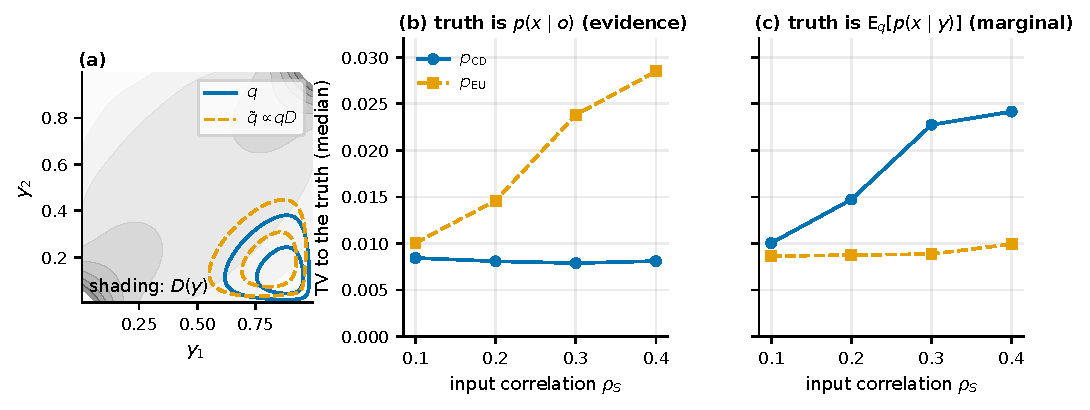
\includegraphics[width=\linewidth]{F1_semantics.pdf}
\caption{Two questions, two exact answers (illustration, not a study result; $k=2$, full tensor model, $m=4$, population coefficients). (a) Under $\pcd$ the belief $q$ is multiplied by the neuron's input density $D$ (shading, darker is larger), giving $\tilde q$; the two inputs here report conflicting evidence. (b) If the belief is per-input evidence about an observation $o$, $\pcd$ matches $p(x\mid o)$ up to truncation. (c) If the inputs really follow $q$, $\peu$ matches. Medians over 200 observations at noise level $\tau=1$; the flat floor near \V{sem.evidence.cd.0.4.1.0} is the truncation error of the degree-4 model.}
\label{fig:idea}
\end{figure}

The contributions are as follows.
\begin{itemize}
\item \textbf{What the two forms compute} (Section~\ref{sec:semantics}). We state and prove the semantic reading for moment-vector messages, including the missing-input case, and observe that any model that normalises after averaging has the same structure. The mathematics of uncertain evidence is classical \citep{jeffrey1965logic,pearl1988probabilistic,chan2005revision}, and we say where. What is new is the application to these messages. As far as we could find, this reading has not been stated for moment or kernel messages.
\item \textbf{How large the gap is} (Section~\ref{sec:gap}). An exact expansion under a flat belief explains why the gap is second order in the pair basis and first order in the triple basis, and closed forms explain the pattern of a pre-registered hypothesis that was not supported as a single power law.
\item \textbf{When the reference and the message fail} (Section~\ref{sec:fail}). We give a positive semidefinite form of the pair denominator with a convex bound on the negativity onset, an exact corner formula for the triple basis, a formula for $\Eq[D]$ that explains why pair messages survive where triple messages do not, and the sample size needed under noise.
\item \textbf{A pre-registered measurement} (Section~\ref{sec:study}). All \V{hyp.total} frozen outcomes are in Table~\ref{tab:hyp}, with their verdict words, many of them unfavourable. Post hoc analyses of the same data show that truncation, not the denominator, usually sets the error.
\end{itemize}

We do not claim that either form is right in general, nor that the flip of Figure~\ref{fig:idea} persists at large $k$: at $k=4$ and $8$ truncation hides it (Section~\ref{sec:illus}). The study's reference and its metric names were fixed before the semantic reading was worked out, and the frozen design tests only one of the two semantics.

\section{Setting}\label{sec:setting}

\textbf{The neuron.} HCR works on variables normalised to $[0,1]$, for instance by their marginal distribution functions, so the object modelled is a copula density \citep{sklar1959fonctions,nelsen2006introduction}. Let $f_0\equiv 1$ and $f_p(u)=\sqrt{2p+1}\,P_p(2u-1)$ be the orthonormal shifted Legendre polynomials on $[0,1]$, and $f_{\mathbf{j}}(y)=\prod_l f_{j_l}(y_l)$ for a multi-index $\mathbf{j}$. A neuron with output $x$ and inputs $y=(y_1,\dots,y_k)$ models
\begin{equation}\label{eq:neuron}
N(x,y)=\sum_{i=0}^{m} f_i(x)\,A_i(y),\qquad A_i(y)=\sum_{\mathbf{j}} a_{i\mathbf{j}}\,f_{\mathbf{j}}(y),
\end{equation}
with degree at most $m$ per variable and $a_{00}=1$. The coefficients are mixed moments, estimated by $\hat a_{i\mathbf{j}}=\frac1n\sum_t f_i(x_t)f_{\mathbf{j}}(y_t)$ \citep{duda2024biology}. All coefficients are too many for large $k$, so a neuron keeps only multi-indices with few nonzero entries among the $k+1$ variables: at most two (\emph{pair}) or three (\emph{triple}). Row $i=0$ thus has up to two or three active inputs, and rows $i>0$ one less. For $k=32$, $m=4$ this gives \V{coef.pair} and \V{coef.triple} coefficients. Integrating over $x$ removes all rows $i>0$, so
\begin{equation}
D(y):=\int_0^1 N(x,y)\,dx=A_0(y)
\end{equation}
is the neuron's model of the input density, and $h_x(y)=N(x,y)/D(y)$ its conditional of $x$ given $y$.

\textbf{Two updates.} Given a belief $q$ on the inputs, define
\begin{equation}\label{eq:exact}
\peu(x)=\Eq\!\left[\frac{N(x,y)}{D(y)}\right],
\qquad
\pcd(x)=\frac{\Eq[N(x,y)]}{\Eq[D(y)]}=\frac{\sum_i f_i(x)\sum_{\mathbf{j}} a_{i\mathbf{j}} b_{\mathbf{j}}}{\sum_{\mathbf{j}} a_{0\mathbf{j}} b_{\mathbf{j}}},\quad b_{\mathbf{j}}=\Eq[f_{\mathbf{j}}(y)].
\end{equation}
$\pcd$ is Eq.~10 of \citep{duda2024biology}. It sees $q$ only through the moments $b_{\mathbf{j}}$, costs one matrix--vector product, and integrates to $1$ whenever $\Eq[D]\neq0$. $\peu$ needs $D$ to be nonzero on the support of $q$ and an integral over $y$ per output point. The label EU comes from the frozen name \emph{exact, uncalibrated}: there ``exact'' means that the integral is evaluated without replacing the denominator, and we keep the label only as a name. In the text we call $\peu$ the \emph{marginal-preserving} form, for the reason given by Theorem~\ref{thm:sem}.

\textbf{Negativity and calibration.} A truncated orthogonal expansion of a density need not be nonnegative. Orthogonal-series density estimation has a long history \citep{cencov1962evaluation,schwartz1967estimation,kronmal1968estimation,efromovich2010orthogonal}, and corrections that turn an estimator into a bona fide density are known \citep{gajek1986improving,glad2003correction}. The HCR paper proposes a calibration, for example $\max(\rho,0.1)$ or a softplus followed by normalisation, and says that in neural use it is mostly neglected, as the resulting approximations should be compensated during training; likelihood evaluation needs a positive density \citep[Secs.~II-A, IV]{duda2024biology}. This is separate from the constant denominator. The same paper states that step as an approximation \citep[Sec.~II-C]{duda2024biology}, and notes that the denominator of its prediction formula can be removed given further inter-layer normalisation \citep[Sec.~II-B]{duda2024biology}. We keep the two issues apart throughout.

\section{What the two forms compute}\label{sec:semantics}

The semantic reading of this section is post hoc: it was worked out after the study was frozen and run, and it changes no verdict. Proofs are in Appendix~\ref{app:proofs}. Here $N\geq0$ is a joint density, $D>0$ on the support of $q$, and $q$ is a bounded density; the signed case comes after the theorem.

\begin{theorem}[What $\pcd$ and $\peu$ compute]\label{thm:sem}
Write $\tilde q=qD/\Eq[D]$.
\begin{enumerate}[label=(\alph*)]
\item \emph{Evidence.} Add a binary variable $E$ with $P(E=1\mid x,y)=c\,q(y)$, conditionally independent of $x$ given $y$, for a constant $0<c\leq1/\sup q$. Under the model $N$, $p(x\mid E=1)=\pcd(x)$ and $p(y\mid E=1)=\tilde q(y)$.
\item \emph{Marginal.} $q(y)h_x(y)$ is the unique joint density with input marginal $q$ and the model's conditional. Its output marginal is $\peu$.
\item \emph{Same conditional, different belief.} $\pcd=\int h_x\,\tilde q\,dy$ and $\peu=\int h_x\,q\,dy$.
\item \emph{Conversion.} If $\Eq[1/D]<\infty$, then $\pcd[q/D]=\peu[q]$ and $\peu[qD]=\pcd[q]$, with beliefs normalised.
\end{enumerate}
\end{theorem}

Part (a) is Pearl's virtual evidence \citep{pearl1988probabilistic}: $q$ acts as a likelihood, $D$ as the prior, and $\tilde q$ as the posterior. Its numerator $\Eq[N]=\int N q\,dy$ is the sum-product message \citep{kschischang2001factor} from the factor $N$ to $x$ when the incoming message on $y$ is $q$. Part (b) is Jeffrey's rule \citep{jeffrey1965logic,diaconis1982updating}. Both obey probability kinematics, as (c) shows, and differ only in how the evidence is specified \citep{chan2003revision}. Part (d) is the classical translation between them (Theorem~5 of \citep{chan2005revision}, as described in \citep{peng2010uncertain}). So the question ``how accurate is $\pcd$?'' has no answer until one says what $q$ means.

\textbf{Signed models.} Without $N\geq0$ the identities in (c), (d) remain algebraically true wherever the denominators are nonzero, but $\tilde q$ is a signed measure and the probabilistic reading is lost. This matters from Section~\ref{sec:fail} on.

\begin{proposition}[Evidence channels and missing inputs]\label{prop:chan}
Let the model have uniform one-dimensional input marginals.
\begin{enumerate}[label=(\alph*)]
\item Let observations $o_l$ of the inputs be independent given $y$, with likelihoods $\lambda_l(y_l)$. Then the product of per-input posteriors $q=\prod_l q_l$, $q_l\propto\lambda_l$, gives $\pcd[q]=p(x\mid o)$. In general $\peu[q]\neq p(x\mid o)$.
\item If instead $q^\ast=p(y\mid o)$ is the joint posterior, then $\peu[q^\ast]=p(x\mid o)$, and $\pcd[q^\ast]$ counts the prior $D$ twice.
\item Let input block $A$ be observed at $y_A$ and block $B$ be missing, with belief a point mass on $y_A$ and flat on $y_B$. Then $\pcd$ is the model's conditional $p(x\mid y_A)$. $\peu=\int p(x\mid y_A,y_B)\,dy_B$ ignores the dependence of $y_B$ on $y_A$ and in general differs from it.
\end{enumerate}
\end{proposition}

Part (c) is the source paper's rule for missing variables, which uses only coefficients with zero index for them \citep[Sec.~II-A]{duda2024biology}. So the source paper's stated target for Eq.~10 is the marginal-preserving form, while its missing-data rule is the evidence form, and the same contraction serves both. Part (b) has a consequence for depth: a density passed forward through a chain is a predictive marginal of a hidden variable, which already contains that variable's prior. The matching form at the next layer is then $\peu$, and the study's ground truth takes that view.

\begin{proposition}[Any model that normalises after averaging]\label{prop:any}
Let $g\geq0$ on $\mathcal X\times\mathcal Y$ and $Z(y)=\int g\,dx>0$. Then
$\Eq[g]/\Eq[Z]=\int (g/Z)\,d\tilde q$ with $d\tilde q\propto Z\,dq$. If $g$ is integrable, this is virtual evidence in the joint model $p\propto g$, whose input density is proportional to $Z$.
\end{proposition}

So a softmax classifier whose exponentiated logits are averaged before normalising implicitly tilts the belief by $Z=\sum_x\exp(\text{logit}_x)$, the unnormalised input density of the energy-based reading of \citet{grathwohl2020classifier}; squared density models \citep{rudi2021psd,tsuchida2023squared} behave the same way. Linearity of $N$ in the coefficients adds only one thing, the closed-form contraction with the moment vector.

\textbf{The gap.} The remaining question is how far apart the two answers are. Let $\CV(D)=\sd_q(D)/\Eq[D]$. The first equality below is the classical covariance identity for a ratio of means \citep{hartley1954unbiased,schochet2022design}, applied pointwise in $x$.

\begin{proposition}[Gap]\label{prop:gap}
Assume $\Eq[D]>0$ and $D\neq0$ $q$-a.s., and let $C_1=\sup_y\int|h_x(y)|\,dx$ over the support of $q$. For every $x$,
\begin{equation}\label{eq:identity}
\pcd(x)-\peu(x)=\frac{\Cov_q(h_x,D)}{\Eq[D]},
\end{equation}
\begin{equation}\label{eq:tvbound}
\TV(\pcd,\peu)=\frac{\CV(D)}2\int|\mathrm{corr}_q(h_x,D)|\,\sd_q(h_x)\,dx\;\leq\;\frac{\CV(D)}2\Big(\sum_{i\geq1}\Var_q(A_i/D)\Big)^{1/2},
\end{equation}
and also $\TV(\pcd,\peu)\leq C_1\TV(\tilde q,q)\leq\frac12C_1\CV(D)$, with $C_1=1$ for a nonnegative conditional. The gap vanishes if $x$ and $y$ are independent under the model, or if $D$ is constant on the support of $q$.
\end{proposition}

The bound in terms of $\CV(D)$ alone is the cheap diagnostic. It is loose: on the production data $\dden$ never exceeded half of $\CV(D)$ over \V{ph.bound.n} defined rows, and the median ratio was \V{ph.bound.med} (post hoc). Keeping the term in $\sd_q(h_x)$ makes the bound \V{tvb.gain} times tighter in median over \V{tvb.n} population cases, with median ratio \V{tvb.sharp} and maximum \V{tvb.sharpmax}. What remains is the correlation of $h_x$ with $D$, and that is exactly what the next section computes.

\subsection{Illustration at small \texorpdfstring{$k$}{k}}\label{sec:illus}

To see the theorem at work, take a Gaussian teacher (type SUM, defined in Section~\ref{sec:study}), population coefficients, $m=4$, and correlation below the negativity onset. An observation $o=s+\tau e$ of the inputs' normal scores defines three problems. In the \emph{evidence} problem the belief is the product of per-input posteriors and the truth is $p(x\mid o)$. In the \emph{posterior} problem the belief is the joint posterior with the same truth. In the \emph{marginal} problem the inputs really follow the product belief, and the truth is $\Eq[p(x\mid y)]$. All truths are closed forms. This is an illustration of the proved statements, labelled as such, and not a study result.

At $k=2$, $\rs=0.4$, $\tau=1$ the median TV to the truth is \V{sem.evidence.cd.0.4.1.0} for $\pcd$ against \V{sem.evidence.eu.0.4.1.0} for $\peu$ in the evidence problem, \V{sem.posterior.cd.0.4.1.0} against \V{sem.posterior.eu.0.4.1.0} in the posterior problem, and \V{sem.marginal.cd.0.4.1.0} against \V{sem.marginal.eu.0.4.1.0} in the marginal problem (Figure~\ref{fig:idea}, Table~\ref{tab:sem}). The order flips as Theorem~\ref{thm:sem} says. It is weaker at $\tau=0.5$, where the belief is narrower. With a missing input at the same correlation the medians are \V{sem.miss.cd.0.4} against \V{sem.miss.eu.0.4}. At $k=4$ and $8$ (pair basis, below the onset), truncation error of \V{sem.big.lo} to \V{sem.big.hi} swamps the contrast, and $\pcd$ is closer than $\peu$ under all three semantics in most rows, including \V{sem.big.marg.closer.lo} to \V{sem.big.marg.closer.hi} of rows in the marginal problem (Table~\ref{tab:sembig}). The flip is thus a proved property of a model without truncation error, seen at $k=2$, and it is not visible at larger $k$ with a truncated basis.

\section{How large the gap is}\label{sec:gap}

We now compute the covariance of Proposition~\ref{prop:gap} under the flat belief $u$, the case of the frozen hypothesis H1c. The flat belief with correlated inputs is out of distribution for the neuron, so it is a test bed here and not a use case. Write $G=D-1$, $R=N-D=\sum_{i\geq1}f_iA_i$, and $\chi_D^2=\Eu[G^2]=\sum_{\mathbf{j}\neq0}a_{0\mathbf{j}}^2$, the squared distance of $D$ from flat. Since $\Eu[D]=1$, $\chi_D=\sd_u(D)$.

\begin{proposition}[Flat belief, exact expansion]\label{prop:flat}
If $D>0$ on the cube, with $T_1=\Eu[GR]$ and $\tau_h=\sup_y\TV(h_\cdot(y),1)$,
\begin{equation}\label{eq:flat}
\pcd-\peu=T_1-\Eu[G^2(h_x-1)],\qquad\big|\TV(\pcd,\peu)-\tfrac12\|T_1\|_1\big|\leq\chi_D^2\,\tau_h.
\end{equation}
\begin{enumerate}[label=(\alph*)]
\item \emph{Pair basis, flat input marginals.} Rows $i\geq1$ hold single-input terms and $G$ holds two-input terms, so $T_1\equiv0$ and $\TV(\pcd,\peu)\leq\chi_D^2\tau_h$. Further, $\pcd-\peu=-T_2+\Eu[G^3(h_x-1)]$ with $T_2=\Eu[G^2R]$, and the remainder has $L^1$ norm at most $2\tau_h\|G\|_\infty\chi_D^2$.
\item \emph{Triple basis.} Rows $i\geq1$ hold two-input terms, which meet those of $G$: $T_1=\sum_{i\geq1}f_i\sum_{\mathbf{j}}a_{0\mathbf{j}}a_{i\mathbf{j}}$ over two-input indices $\mathbf{j}$. The gap is first order.
\end{enumerate}
\end{proposition}

Numerically the pair orthogonality holds to \V{orth.pair}. With sampled coefficients single-input terms appear in $G$, but only at noise level.

\begin{corollary}[Closed forms, equicorrelated Gaussian copula]\label{cor:closed}
Let inputs have correlation matrix with off-diagonal $r$, couplings $c_l$ to $x$, and population coefficients. Let $A_{pq}=\mathrm{E}[f_p(y_1)f_q(y_2)]$ for $p,q\geq1$, $B_{ip}(c)=\mathrm{E}[f_i(x)f_p(y)]$ at correlation $c$, $C^{ll'}_{i,pq}=\mathrm{E}[f_i(x)f_p(y_l)f_q(y_{l'})]$, and $e_p=\int f_p(u)\,f(u)^\top A^2f(u)\,du$ with $f=(f_1,\dots,f_m)$. Then
\begin{equation}\label{eq:closed}
T_2=(k-1)\sum_{l}\sum_{i,p\geq1}f_i(x)\,B_{ip}(c_l)\,e_p\ \ \text{(pair)},\qquad
T_1=\sum_{l<l'}\sum_{i\geq1}f_i(x)\,\langle A,C_i^{ll'}\rangle\ \ \text{(triple)}.
\end{equation}
Odd $p$ have $e_p=0$, so the sign of $c_l$ drops out of $T_2$, and $T_2$ has no $f_1$ term: at this order the variance of $\pcd$ moves and its mean does not.
\end{corollary}

These formulas read the frozen H1c result. That hypothesis asked whether $\dden$ under S2 is one power law of $\chi_D$ per (type, basis). Reading off the leading orders (a reading, not a proved rate): in the pair basis $T_2\sim k^2\rs^2c^2\propto\chi_D^2c^2$, which carries $c^2$ and hence $k$, so no single function of $\chi_D$ fits. In the triple basis with type SUM, $T_1\sim k^2\rs c^2$ with $c^2$ a function of $k\rs$ over $k$, so where the coupling is not clipped $\dden$ is a function of $k\rs$, and $\chi_D$, which is of order $k\rs$, collapses the data. This is the one cell supported (share of points within a factor 2: \V{H1c.SUM/triple}). In CONTRAST the signs give $\sum_{l<l'}s_ls_{l'}=-k/2$, so $T_1\sim k\rs c^2$ and $k$ returns. Table~\ref{tab:lead} and Figure~\ref{fig:scaling} compare $\frac12\|T_2\|_1$ (pair) and $\frac12\|T_1\|_1$ (triple) with the \V{lead.n} points of H1c: with no fitted constant all lie within a factor 2, with ratios \V{lead.lo} to \V{lead.hi}, and \V{lead.small.lo} to \V{lead.small.hi} on the \V{lead.small.n} points with $\chi_D\leq0.2$. This post hoc comparison does not change the verdict of H1c.

\begin{figure}[t]
\centering
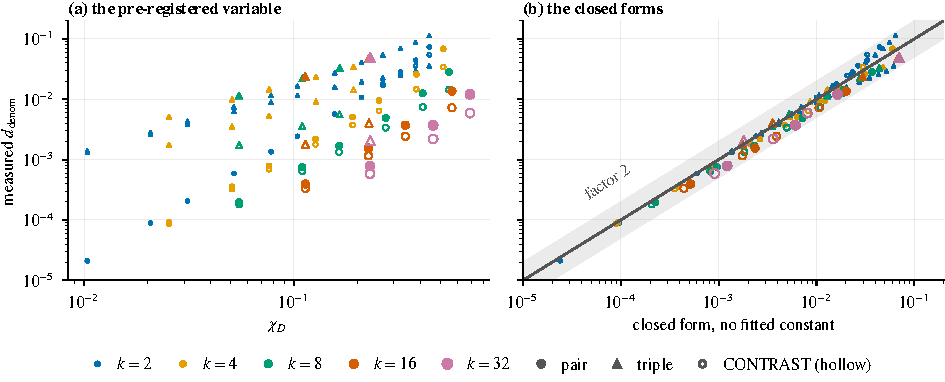
\includegraphics[width=0.86\linewidth]{F2_scaling.pdf}
\caption{Why a single power law in $\chi_D$ fails and what replaces it (population coefficients, S2, $m=4$, the \V{lead.n} points of H1c). (a) Measured $\dden$ against $\chi_D$: the triple SUM cell collapses and the others separate by $k$. (b) The same points against the closed forms of Corollary~\ref{cor:closed}, with no fitted constant. The band is a factor 2. Post hoc.}
\label{fig:scaling}
\end{figure}

\begin{proposition}[Data belief and the pair structure]\label{prop:data}
Assume uniform marginals and population coefficients, and let $q$ be the true input density. Then $\Eq[D]=1+\chi_D^2$, and the true propagated density is uniform. In the pair basis $\pcd\equiv1$, which is that density. In the triple basis $\pcd-1=T_1/(1+\chi_D^2)$, a real deviation. More generally, in the pair basis for any belief,
\begin{equation}\label{eq:pairstruct}
\pcd(x)=1+\frac{1}{\Eq[D]}\sum_{l}\sum_{i,p\geq1}f_i(x)\,a_{i,(l,p)}\,\mathrm{E}_{q_l}[f_p],
\end{equation}
so a pair neuron sees the belief only through its one-dimensional marginals $q_l$ and the scalar $\Eq[D]$.
\end{proposition}

Thus $T_1$ is both the first-order gap under the flat belief and the whole error under the data belief. On the \V{db.n} triple population points above the Monte Carlo level, measured $\dtot$ divided by $\frac12\|T_1\|_1/(1+\chi_D^2)$ lies between \V{db.lo} and \V{db.hi}. In the pair basis the denominator reaches the output only as a scalar, which limits what training $D$ can do to $\pcd$.

\section{When the reference and the message fail}\label{sec:fail}

Everything above needs $D>0$ on the support of $q$. Here we say when that fails, for the equicorrelated Gaussian copula and population coefficients, and then under noise. The key is a latent form. Write $Z_l=\sqrt r\,W+\sqrt{1-r}\,e_l$ for the normal scores, let $g(w)=\mathrm{E}[f(y)\mid W=w]$ with $f=(f_1,\dots,f_m)$, and let $\xi_l(w)=g(w)^\top f(y_l)$. The untruncated density is $\EW\prod_l(1+\xi_l)$ with all degrees present, which is nonnegative. The neuron keeps
\begin{equation}\label{eq:latent}
D_{\mathrm{pair}}=1+\EW[e_2(\xi)],\qquad D_{\mathrm{triple}}=1+\EW[e_2(\xi)+e_3(\xi)],
\end{equation}
with $e_d$ the elementary symmetric polynomials. Truncating the product in this way is what gives up positivity.

\begin{proposition}[Pair basis: a positive semidefinite form]\label{prop:pair}
Let $A=\EW[gg^\top]$, so $0\preceq A\preceq rI$; let $\varphi(u)=f(u)^\top Af(u)$, $S=\sum_lf(y_l)$ and $\Theta=m(m+2)$. Then
\begin{equation}\label{eq:quad}
D_{\mathrm{pair}}(y)=1+\tfrac12S^\top AS-\tfrac12\sum_l\varphi(y_l).
\end{equation}
\begin{enumerate}[label=(\alph*)]
\item $\min D\geq1-\frac k2\max_u\varphi(u)$, and $D>0$ on the cube whenever $r<2/(k\Theta)$, that is $\rs<\frac6\pi\arcsin\frac1{k\Theta}$.
\item $\min D\geq\min_\mu\Psi_k(\mu)$ with $\Psi_k(\mu)=1+\frac{k^2}2s_\mu^\top As_\mu-\frac k2\int\varphi\,d\mu$, $s_\mu=\int f\,d\mu$, a convex problem over probability measures on $[0,1]$.
\end{enumerate}
\end{proposition}

The form shows what drives negativity: the term $-\frac12\sum_l\varphi(y_l)$ is linear in $k$, and the first term penalises any $y$ whose $f(y_l)$ do not cancel in the directions of $A$. The bound (b), certified by a Frank--Wolfe duality gap on a grid of $1001$ nodes, is close to the truth (Table~\ref{tab:onset}): within \V{on.gap4} of the measured onset for $k\geq4$ at $m=4$, and \V{on.gap} over all $m$; it is loose at $k=2$. Its minimiser is not a corner. At $k=32$, $m=4$ the optimal measure has atoms at $0$, \V{on.atoms.k32}, \V{on.atoms.k32b} and $1$. The product $k\rs^\ast$ rises from \V{on.kr.pair.lo} to \V{on.kr.pair.hi} over $k\geq4$, so the onset is near $1/k$ but not exactly of that order in our range. The form needs only conditional independence given a latent variable, so $A\succeq0$, (b) and the first bound in (a) extend to exchangeable families that have such a representation; $A\preceq rI$ is specific to the Gaussian case.

\begin{proposition}[Corners]\label{prop:corner}
Let $\xi_+=g^\top f(1)$, $\xi_-=g^\top f(0)$, and let $M_2=\EW\xi_+^2$, $C_2=\EW\xi_+\xi_-$, $M_3=\EW\xi_+^3$, $C_3=\EW\xi_+^2\xi_-$. At a corner with $n$ coordinates at $1$,
\begin{align}
D_{\mathrm{pair}}(n)&=1+\big[\tbinom n2+\tbinom{k-n}2\big]M_2+n(k-n)C_2,\label{eq:cornerp}\\
D_{\mathrm{triple}}(n)&=D_{\mathrm{pair}}(n)+\big[\tbinom n3+\tbinom{k-n}3\big]M_3+\big[\tbinom n2(k-n)+n\tbinom{k-n}2\big]C_3.\label{eq:cornert}
\end{align}
With $a=\frac12(M_2+C_2)\geq0$ and $b=\frac12(M_2-C_2)\geq0$, the energies of the even and odd degrees, $D_{\mathrm{pair}}(n)=1+\frac12[k(k-1)a+((2n-k)^2-k)b]$. Any $\rs$ at which $\min_nD(n)<0$ is at or above the onset.
\end{proposition}

So the balanced corner $n=k/2$ cancels only the odd degrees. Even polynomials have the same sign at $0$ and $1$ and add $\frac12k(k-1)a$, which is why the balanced-corner picture fails for the pair basis: over a grid of $\rs$, all $m$ and even $k$ up to $4096$, the balanced pair corner stays at or above \V{cor.min}, and no pair corner reached negative values in the study's range. The triple term changes this. With $\xi_+=\xi_e+\xi_o$ split into parts even and odd in $w$ and $h=k/2$, it adds $h(h-1)\big[\frac{4h-2}{3}\EW\xi_e^3-2\EW\xi_e\xi_o^2\big]$, a negative term of the same order in $kr$ as the others. For $m\geq4$ the balanced corner then matches the measured triple onset within \V{on.tri.gap} (Table~\ref{tab:onset}), and at $m=2$ no triple corner goes negative, so the formula gives no bound there.

\begin{figure}[t]
\centering
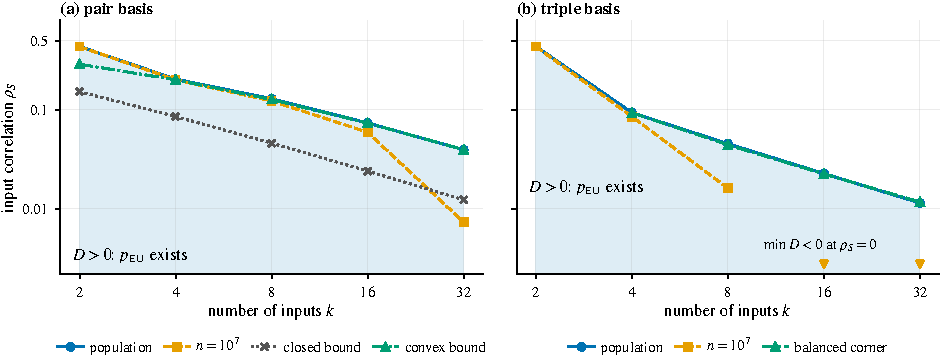
\includegraphics[width=0.86\linewidth]{F3_existence.pdf}
\caption{Where the marginal-preserving reference exists (type SUM, S2, $m=4$). Shading: $D>0$ on the cube at population level, below the measured onset. (a) Pair basis with the closed and convex lower bounds of Proposition~\ref{prop:pair}. (b) Triple basis with the balanced corner of Proposition~\ref{prop:corner}, which lies on the population curve. At $n=10^7$ noise moves the onset down, and triangles mark triple cells with $\min D<0$ already at $\rs=0$. Measured onsets are upper bounds (Section~\ref{sec:design}).}
\label{fig:exist}
\end{figure}

\begin{table}[t]
\centering
\small
\begin{tabular}{rrrrrr}
\toprule
$k$ & pair: closed & pair: convex & pair: measured & triple: corner & triple: measured \\
\midrule
2 & 0.152 & 0.289 & 0.437 & --- & --- \\
4 & 0.085 & 0.201 & 0.204 & 0.093 & 0.094 \\
8 & 0.046 & 0.127 & 0.129 & 0.044 & 0.045 \\
16 & 0.024 & 0.073 & 0.074 & 0.022 & 0.023 \\
32 & 0.012 & 0.039 & 0.039 & 0.012 & 0.011 \\
\bottomrule
\end{tabular}

\caption{Negativity onset in $\rs$ with population coefficients, type SUM, $m=4$ (post hoc for the bounds). ``closed'' and ``convex'': lower bounds of Proposition~\ref{prop:pair}(a, b). ``corner'': value of Proposition~\ref{prop:corner}. Measured values come from interpolation on the study grid and are upper bounds, so small inversions are possible. Other degrees: Table~\ref{tab:onsetall}.}
\label{tab:onset}
\end{table}

\textbf{The message.} $\pcd$ needs only $\Eq[D]\neq0$, a weaker condition than $D>0$ on the support.

\begin{proposition}[Mass of the message]\label{prop:mass}
Let $q$ be a product belief with $b_l=\mathrm{E}_{q_l}[f]$, and $\beta_l(w)=g(w)^\top b_l$. Then $\Eq[D]=1+\EW[e_2(\beta)]$ (pair) or $1+\EW[e_2(\beta)+e_3(\beta)]$ (triple). In the pair basis
\begin{equation}\label{eq:masspair}
\Eq[D]=1+\tfrac12\big(\textstyle\sum_lb_l\big)^\top A\big(\sum_lb_l\big)-\tfrac12\sum_lb_l^\top Ab_l\;\geq\;1-\tfrac r2\sum_l|b_l|^2,
\end{equation}
and $\Eq[D]\geq1$ if all $q_l$ are equal. In the triple basis with equal $q_l$, $\Eq[D]=1+\binom k2\EW\beta^2+\binom k3\EW\beta^3$.
\end{proposition}

This explains the asymmetry observed in the study. The formula matches \V{eqd.n} sampled population rows within \V{eqd.rel}. For a central belief the degree-2 moment is negative and $g_2$ is right-skewed, so $\EW\beta^3<0$ and the cubic term drives $\Eq[D]$ negative at large $k$ (this last step is a heuristic reading). In production $\Eq[D]\leq0$ occurred in \V{ph.eqd.nonpos} of \V{ph.eqd.rows} rows, all triple, at $k\geq\V{ph.eqd.mink}$, under Beta beliefs; with population coefficients it occurred too (\V{ph.eqd.pop.nonpos} of \V{ph.eqd.pop.rows} rows), so it is structural. The pair basis stayed at $\Eq[D]\geq\V{ph.eqd.pairmin}$ (population S3c minimum \V{eqd.s3c}). Pair safety is not universal: a point belief on a negative value of $D$ gives $\Eq[D]<0$ in any basis, and the bound in \eqref{eq:masspair} is vacuous for narrow beliefs. The statement ``$\pcd$ stays defined past the onset'' therefore holds for pair neurons with the beliefs tested, and not for triple neurons.

\textbf{Noise.} Estimated coefficients move all of this.

\begin{proposition}[Sampling noise at independence]\label{prop:noise}
Let the inputs be independent and uniform. Then $\mathrm{E}\hat D(y)=1$ and $\Var\hat D(y)=K(y)/n$ with $K(y)=\sum_{\mathbf{j}\neq0}f_{\mathbf{j}}(y)^2$, maximal at corners, where $K_{\mathrm c}=k\Theta+\binom k2\Theta^2$ (pair) or $K_{\mathrm c}=k\Theta+\binom k2\Theta^2+\binom k3\Theta^3$ (triple). In the Gaussian limit of $\sqrt n(\hat a_{0\mathbf{j}})$ at fixed $k$, write $1-\min\hat D=z\sqrt{K_{\mathrm c}/n}$. For fixed $m$ even, $\mathrm{E}z$ lies between $c\sqrt k$ and $C\sqrt{km}$ for absolute constants $c,C>0$ (with $c$ valid for $k\geq k_0$), over corners $\mathrm{E}z\leq\sqrt{2k\ln2}$, and $z$ concentrates around its mean with $O(1)$ fluctuations. Hence $\hat D>0$ needs $n\asymp z^2K_{\mathrm c}$, of order $k^3$ (pair) and $k^4$ (triple) up to factors in $m$.
\end{proposition}

This replaces the rule of thumb $n\gtrsim z^2K$ by a statement on how $z$ grows. In production $z$ grows from \V{ph.noise.zmin} to \V{ph.noise.zmax} (Table~\ref{tab:noisez}). In a Gaussian surrogate, a search over the cube at $k=32$ reaches \V{nz.pair32.cube} and over corners \V{nz.pair32.corner}, against \V{nz.pair32.meas} measured, consistent with $\min D$ being an upper bound. With the cube values, $z^2K_{\mathrm c}$ is \V{nz.need.pair32} for pair at $k=32$ and \V{nz.need.triple16} for triple at $k=16$, either side of the study's $n=10^7$. In the pair basis the noise minimisers put \V{nz.bound.lo}--\V{nz.bound.hi} of coordinates on the boundary, while the population pair minimum has interior atoms.

\section{The pre-registered study}\label{sec:study}

\subsection{Design}\label{sec:design}

The design, hypotheses, decision rules, grids and budget rule were frozen in a version-controlled pre-registration (file \texttt{PREREGISTRATION.md}, commit \texttt{6a98646}) before any production job. It is a git record, not an entry in a public registry. A pilot run before the freeze to measure throughput only (seed index 1000) is excluded from all results. The Deviations section of the file is empty. Analyses marked \emph{post hoc} were not pre-registered and enter no verdict. The frozen design tests the marginal reading only; Sections~\ref{sec:semantics}--\ref{sec:fail} came later. Full definitions are in Appendix~\ref{app:defs}.

\textbf{Ground truth.} Output and inputs are uniform; dependence comes from a $(k+1)$-dimensional copula. The Gaussian sweep has equicorrelated inputs with correlation $r=2\sin(\pi\rs/6)$, so $\rs$ is the Spearman correlation between inputs. In \textbf{SUM} each input has correlation $c=\min(0.5,\,0.8\sqrt{(1+(k-1)r)/k})$ with $x$. In \textbf{CONTRAST} half the inputs have $+c$ and half $-c$, with $c=\min(0.5,\,0.8\sqrt{(1-r)/k})$. Other experiments use $t$, Clayton and Gumbel copulas and random LKJ correlation matrices (Appendix~\ref{app:grids}).

\textbf{Beliefs.} Beliefs are product distributions unless stated. \textbf{S2} is flat. \textbf{S3a} is Beta$(3,3)$ per input, \textbf{S3b} is Beta$(4,2)$, \textbf{S3c} alternates Beta$(4,2)$ and Beta$(2,4)$ (conflicting evidence), and \textbf{S3d} is the narrow Beta$(6,6)$. \textbf{S4} is the true input copula (data belief). \textbf{S1}, the neuron's own $D$, is computed but not primary. The primary beliefs are S2, S3c and S4. S2 is not the data distribution, so part of its error against the ground truth is mismatch between prior and data.

\textbf{Compared densities.} Monte Carlo with $M=\V{cfg.M}$ samples in $R=\V{cfg.R}$ replicate blocks gives $\pcd$; $\peu$, defined only if $D\geq\V{cfg.floor}$ on the support of $q$; $\pec$, the conditional calibrated per input as $\max(N,\varepsilon)$ divided by its integral ($\varepsilon\in\{0.1,0.01,0.001\}$, primary $0.01$); and the ground truth $\pg=\Eq[p(x\mid y)]$, the analytic conditional of the teacher averaged over $q$. So the truth is the Jeffrey answer, and under it $\peu$ is the form that matches: all ``errors'' below carry that semantics. A joint normalising constant cancels in a conditional, so $\pec$ is also the conditional of the jointly clipped density.

\textbf{Outcomes.} Outcomes are total-variation distances $\TV(p,r)=\frac12\int|p-r|$ on raw, never renormalised densities:
\begin{align*}
\dden&=\TV(\pcd,\peu), & \dneg&=\TV(\peu,\pec), & \dmu&=\TV(\peu,\pg),\\
\dmc&=\TV(\pec,\pg), & \dtot&=\TV(\pcd,\pg), & \ddc&=\TV(\pcd,\pec).
\end{align*}
Densities can be signed, so TV here is an $L^1$ distance with a factor $\frac12$ and can exceed $1$. We also record variance and mean errors, $P(D<0)$ under uniform $y$, $\chi_D$, and $\min D$ from a multi-start projected optimiser with $\V{cfg.starts}$ starts. This $\min D$ is an upper bound on the true minimum, so measured onsets are conservative: true onsets can only be earlier.

\textbf{Thresholds and verdicts.} Each seed re-estimates all coefficients. A threshold $\rs^*(c)$ is the first crossing of level $c$ by the seed-median curve, over the run of defined points from $\rs=0$. If the curve becomes undefined first, or $c$ is not reached by $\rs=0.9$, the entry is ``---''. The negativity onset is the first zero crossing of seed-median $\min D$, and $0$ if negative at $\rs=0$. Confidence intervals are percentile bootstraps over seeds \citep{efron1979bootstrap,efron1993introduction} ($B=2000$); they reflect estimation noise only, so very tight ones do not mean that the quantity is known beyond this design. A hypothesis over cells is \emph{supported} if at least $2/3$ of evaluable cells are significant in the predicted direction, \emph{not supported} if at least $2/3$ are not, and \emph{inconclusive} otherwise or with fewer than three evaluable cells. Some hypotheses have their own rule (Appendix~\ref{app:hyp}). ``Significant'' is used only in this pre-registered sense.

\textbf{Experiments.} \texttt{gauss} crosses $k\in\{2,4,8,16,32\}$, both types, both bases, $m\in\{2,4,6\}$, $n=10^7$, 50 seeds, and 19 values of $\rs$ from 0 to 0.9. \texttt{population} repeats these cells with exact coefficients. \texttt{convergence} doubles $M$, $n$ and two grid sizes on a subset. \texttt{families} and \texttt{lkj} ($k\leq8$) vary the ground truth. \texttt{network} builds chains of up to $L=4$ neurons: a neuron of the sweep, then neurons with two independent inputs, on a Gaussian Markov teacher with correlation $a=\V{cfg.a}$ per layer, with training under three losses and two optimisers at fixed, untuned settings (Appendix~\ref{app:chains}). Altogether \V{jobs} jobs ran with \V{failed} failures on NVIDIA A100-SXM4-40GB GPUs in float64 with TF32 disabled and deterministic algorithms, using \V{gpuh.jobs} GPU-hours of job time (\V{gpuh.billed} GPU-hours billed for everything, including validation and benchmarks).

\begin{table}[t]
\centering
\footnotesize
\begin{tabular}{@{}l>{\raggedright\arraybackslash}p{0.31\linewidth}l>{\raggedright\arraybackslash}p{0.40\linewidth}@{}}
\toprule
 & claim & verdict & evidence \\
\midrule
H1a & population onset falls with $k$ & \emph{supported} & 4/4 cells strictly decreasing \\
H1b & same at $n=10^7$ & \emph{supported} & 4/4; SUM/pair 0.435 ($k=2$) vs 0.007 ($k=32$) \\
H1c & $d_{\mathrm{denom}}$ one power law of $\chi_D$ & \emph{inconclusive} & within factor 2: CONTRAST/pair 0.52, CONTRAST/triple 0.48, SUM/pair 0.55, SUM/triple 1.00 \\
H2a & higher $m$, earlier onset & \emph{supported} & 20/20 \\
H2b & triple earlier than pair (population) & \emph{supported} & 8/8 \\
H2b & triple earlier than pair ($n=10^7$) & \emph{supported} & 8/8 \\
H2c & $d_{\mathrm{denom}}$ depends weakly on $m$ & \emph{inconclusive} & 60\,\% of 221 points; supported needs $\geq 80\,\%$ \\
H3a & onset within $\pm 0.05$ of Gaussian & \emph{not supported} & 21/48 CIs inside, 27 entirely outside \\
H3b & $d_{\mathrm{denom}}$ within factor 2 of Gaussian & \emph{not supported} & 73/236 CIs inside, 156 entirely outside \\
H3c & Gaussian power law predicts LKJ & \emph{not supported} & pair 39\,\%, triple 34\,\% of 272 matrices; $k=2$ only \\
H4a & seed spread exceeds MC error & \emph{supported} & 93\,\% of 114 points; median ratio 2.1 \\
H4b & doubling changes TV $<\max(3\,\mathrm{SE},10^{-3})$ & \emph{not supported} & 5{,}460 violations, all under $n\times 2$ \\
H5a & $d_{\mathrm{total}}$ grows from $L=1$ to 4 & \emph{not supported} & 11/72; 51 significantly below 1 \\
H5b & training reduces $d_{\mathrm{denom}}$ & \emph{not supported} & 5/18; 1 opposite \\
H5c & training reduces $P(D<0)$ & \emph{not supported} & 24/78; 19 opposite \\
H5d & e2e training reduces held-out $d_{\mathrm{total}}$ & \emph{not supported} & 27/192; 84 opposite \\
\bottomrule
\end{tabular}

\caption{All pre-registered outcomes, with the verdict words of the pre-registration. H2b has two pre-registered evaluations, so \V{hyp.total} hypotheses occupy \V{hyp.rows} rows. Fractions count significant cells among evaluable cells; ``opposite'' counts cells whose confidence interval lies entirely on the unpredicted side. H4b is also test M13 of the validation suite (Appendix~\ref{app:validation}).}
\label{tab:hyp}
\end{table}

\subsection{Truncation, not the denominator, usually sets the error}\label{sec:trunc}

We begin with a post hoc reading of metrics that were all pre-registered, because it answers the practical question: would replacing $\pcd$ with $\peu$ help? Table~\ref{tab:trunc} sets the gap $\dden$ against the error of the truncated model $\dmu=\TV(\peu,\pg)$, on rows where both exist, under the semantics where $\peu$ is the matching form. In the pair basis the model error exceeds the gap by a median factor of \V{tr.S4.pair.ratio} (S4) to \V{tr.S3d.pair.ratio} (S3d), and both forms sit at nearly the same distance from the truth, for example \V{tr.S3a.pair.cd} and \V{tr.S3a.pair.eu} under S3a. $\peu$ is closer in \V{tr.S3c.pair.euc} (S3c) to \V{tr.S3b.pair.euc} (S3b) of rows. So for pair neurons replacing $\pcd$ with $\peu$ buys almost nothing here, even under the semantics that favours $\peu$: a pair model with few coefficients cannot represent the conditional well enough for the difference to count.

There are two exceptions, both predicted by Section~\ref{sec:gap}. Triple neurons under S2 and S4 have model error far below the gap, with ratios \V{tr.S2.triple.ratio} and \V{tr.S4.triple.ratio}, and $\peu$ closer in \V{tr.S2.triple.euc} of rows: here $T_1$ is first order and it is the whole error of $\pcd$. Under the Beta beliefs the triple ratio is \V{tr.S3b.triple.ratio} to \V{tr.S3d.triple.ratio}. The illustration of Section~\ref{sec:illus} gives the same message with the evidence truth at $k=4,8$, where truncation of \V{sem.big.lo} to \V{sem.big.hi} hides the choice of form. These results are for $m=4$, $\varepsilon=0.01$, $\rs>0$, and defined rows only. They concern synthetic teachers, where the truncated part of the density is known, and a task could weigh the error differently.

\begin{table}[t]
\centering
\footnotesize
\begin{tabular}{llrrrrrrr}
\toprule
basis & belief & evaluations & $d_{\mathrm{denom}}$ & $\mathrm{TV}(p_{\mathrm{EU}},p_{\mathrm{G}})$ & $\mathrm{TV}(p_{\mathrm{CD}},p_{\mathrm{G}})$ & \multicolumn{1}{c}{ratio} & EU closer & EC beats EU \\
\midrule
pair & S2 & 2{,}902 & 0.0024 & 0.0119 & 0.0144 & 5.3 & 50\,\% & 16\,\% \\
 & S3a & 5{,}037 & 0.0004 & 0.0471 & 0.0472 & 120 & 52\,\% & 24\,\% \\
 & S3b & 6{,}200 & 0.0041 & 0.1063 & 0.1096 & 27.9 & 69\,\% & 38\,\% \\
 & S3c & 3{,}249 & 0.0019 & 0.0690 & 0.0675 & 30.2 & 24\,\% & 8\,\% \\
 & S3d & 7{,}022 & 0.0002 & 0.0824 & 0.0830 & 425 & 67\,\% & 39\,\% \\
 & S4 & 2{,}902 & 0.0002 & 0.0004 & 0.0003 & 2.0 & 41\,\% & 0\,\% \\
\midrule
triple & S2 & 1{,}804 & 0.0117 & 0.0027 & 0.0109 & 0.23 & 100\,\% & 28\,\% \\
 & S3a & 3{,}155 & 0.0015 & 0.0103 & 0.0118 & 7.6 & 55\,\% & 2\,\% \\
 & S3b & 3{,}337 & 0.0085 & 0.0280 & 0.0313 & 5.5 & 66\,\% & 32\,\% \\
 & S3c & 2{,}051 & 0.0021 & 0.0139 & 0.0207 & 7.6 & 29\,\% & 5\,\% \\
 & S3d & 4{,}399 & 0.0006 & 0.0234 & 0.0233 & 32.1 & 62\,\% & 7\,\% \\
 & S4 & 1{,}804 & 0.0127 & 0.0003 & 0.0126 & 0.03 & 100\,\% & 5\,\% \\
\bottomrule
\end{tabular}

\caption{Gap against truncation error, on defined rows with $\rs>0$, $m=4$, $\varepsilon=0.01$; truth is $\pg$, so $\peu$ is the matching form (post hoc). Distances are medians over rows. ``ratio'': median of $\dmu/\dden$ per row. ``EU closer'': share of rows with $\peu$ nearer than $\pcd$ to $\pg$. ``EC beats EU'': share of rows with $\pec$ nearer than $\peu$.}
\label{tab:trunc}
\end{table}

\subsection{The gap, where it can be measured}\label{sec:gapres}

Under S2 the $1\,\%$ threshold of $\dden$ falls from \V{thr.SUM.pair.2.d1} at $k=2$ to \V{thr.SUM.pair.16.d1} at $k=16$ (pair, Table~\ref{tab:thr}, Figure~\ref{fig:d}), while at $k=32$ the entry is empty. Empty does not mean small. It means $\peu$ became undefined (from $\rs=\V{thr.SUM.pair.32.und}$) before the curve reached $1\,\%$. In the triple basis at $k\geq16$ the reference is undefined already at $\rs=0$.

\textbf{H1c (\verdict{\V{H1c.verdict}}).} The share of points within a factor 2 of one power law in $\chi_D$ was \V{H1c.SUM/pair} (SUM/pair), \V{H1c.CONTRAST/pair} (CONTRAST/pair), \V{H1c.SUM/triple} (SUM/triple) and \V{H1c.CONTRAST/triple} (CONTRAST/triple). By the pre-registered rule these cells are respectively \verdict{\V{H1c.verdict.SUM/pair}}, \verdict{\V{H1c.verdict.CONTRAST/pair}}, \verdict{\V{H1c.verdict.SUM/triple}} and \verdict{\V{H1c.verdict.CONTRAST/triple}}. The pre-registration gives this rule per (type, basis) and does not say how the cells combine. The overall label comes from the analysis code frozen at the same commit, which requires all cells to agree. Counting a \emph{supported} cell as significant under the general aggregation rule would instead give \V{H1c.cells.sup} of \V{H1c.cells}, that is \verdict{not supported}. We keep the recorded verdict; the cell pattern is what Corollary~\ref{cor:closed} explains.

\textbf{Selection.} ``Modest where measured'' should not be read as ``modest''. The filter that defines $\dden$ almost implies a modest gap: within it $\CV(D)$ never exceeds \V{sel.cv}, so Proposition~\ref{prop:gap} caps the gap, and $\dden$ has maximum \V{sel.dmax} and $99$th percentile \V{sel.q99}. Under S2 at $k=32$ only \V{sel.k32.pair} of pair rows survive the filter, and the $5\,\%$ level is reached in \V{sel.d5.s2} of \V{sel.d5.s2n} S2 cells and \V{sel.d5.all} of \V{sel.d5.alln} cells over all beliefs. Past the onset the outcome is $\dtot$ and $\ddc$ (Table~\ref{tab:past}): in the pair basis $\dtot$ is \V{past.pair.lo} to \V{past.pair.hi} in median, apart from S4, and $\ddc$ is \V{past.dc.lo} to \V{past.dc.hi}. The narrow belief S3d is the one case where a blank does mean small: at $k=16,32$ it stays defined up to $\rs=\V{ph.narrow.k32.rho}$ and never reaches $1\,\%$. Its seed-median $\dden$ is at most \V{narrow.pair4} for pair at $m=4$, but \V{narrow.triple4} for triple at $m=4$ and \V{narrow.triple2} at $m=2$. Width is not everything: the off-centre S3b reaches $1\,\%$ earlier than S2 at $k\geq8$ (Table~\ref{tab:bel}).

\textbf{What the gap moves.} Among \V{ph.mv.n} points of the pair basis the relative variance error exceeds the standardised mean error at \V{ph.mv.share}. Under S2 the mean is almost untouched (at most \V{ph.mv.s2.mean}) while the variance moves by up to \V{ph.mv.s2.var}, as Corollary~\ref{cor:closed} says.

\subsection{Where the reference exists}\label{sec:onset}

\textbf{H1a, H1b (\verdict{\V{H1a.verdict}}, \verdict{\V{H1b.verdict}}).} The onset falls strictly with $k$ in all \V{H1a.n} population cells, and at $n=10^7$ the difference between $k=32$ and $k=2$ has a confidence interval below zero in all \V{H1b.n} cells. For SUM in the pair basis it falls from \V{H1b.sp.k2} to \V{H1b.sp.k32}, a difference with $95\,\%$ CI $[\V{H1b.sp.lo},\V{H1b.sp.hi}]$. \textbf{H2a (\verdict{\V{H2a.verdict}}).} A higher degree gives an earlier onset in \V{H2a.sig} of \V{H2a.n} population cells (Table~\ref{tab:onsetm}). \textbf{H2b (\verdict{\V{H2b_population.verdict}} with population coefficients, \verdict{\V{H2b_gauss.verdict}} at $n=10^7$).} The triple basis is earlier than pair in \V{H2b_population.sig} of \V{H2b_population.n} and \V{H2b_gauss.sig} of \V{H2b_gauss.n} cells. These four outcomes were close to expected once more terms are added, and Propositions~\ref{prop:pair} and \ref{prop:corner} now give their mechanism. \textbf{H2c (\verdict{\V{H2c.verdict}}).} $\dden$ varied by at most a factor $1.5$ across $m$ at \V{H2c.share} of \V{H2c.n} points, between the rule's $80\,\%$ and $50\,\%$.

Noise moves the onset at large $k$: \V{thr.SUM.pair.32.on} against \V{thr.SUM.pair.32.pop} (pair, $k=32$), and \V{thr.SUM.triple.16.on} against \V{thr.SUM.triple.16.pop} (triple, $k=16$), as Proposition~\ref{prop:noise} predicts. Moving the floor on $D$ from $0$ to $0.05$ changes the share of S2 rows with $\min D$ above it by at most \V{floor.shift} of rows in any cell (post hoc reanalysis), so the frozen floor decides little.

\textbf{H4a (\verdict{\V{H4a.verdict}}).} At \V{H4a.share} of \V{H4a.n} headline points the across-seed standard deviation of $\dden$ exceeded the Monte Carlo standard error, with median ratio \V{H4a.ratio}. Estimation noise, not integration noise, sets the uncertainty.

\textbf{H4b (\verdict{\V{H4b.verdict}}).} Doubling $M$, $n$, or either grid must change every reported TV by less than $\max(3\,\mathrm{SE},10^{-3})$. There were \V{H4b.viol} violations among \V{H4b.total} paired values (\V{H4b.share}), all under $n\times2$, at $k=8$ (\V{H4b.k8}) and $k=32$ (\V{H4b.k32}). The worst ratio of change to tolerance is \V{H4b.worst.n2} for $n\times2$ and \V{H4b.worst.other} over the other variants (Table~\ref{tab:conv}). Numerical integration is converged and, at large $k$, the estimator is not: \V{ph.h4b.triple} of violations are triple, with median relative change \V{ph.h4b.rel} (post hoc). The largest absolute change, \V{H4b.maxchange}, is from \V{ph.h4b.worst.from} to \V{ph.h4b.worst.to}, at $k=32$, triple, $m=6$, S3d, a signed output. Such high-$k$ triple cells are stress tests. They stay in the record and in the tables, but say little about usable neurons.

\subsection{Clipping changes outputs more, and usually for the worse}\label{sec:clip}

Where $\dden$ and $\dneg$ both exist and at least one is above the noise floor (\V{ph.dvn.n} points), $\dneg>\dden$ at \V{ph.dvn.0.01} of points (\V{ph.dvn.0.1} for $\varepsilon=0.1$, \V{ph.dvn.0.001} for $\varepsilon=0.001$; post hoc). But $\dneg$ is movement, not harm. Against the truth, $\pec$ beats $\peu$ in only \V{clip.min} to \V{clip.max} of defined rows across beliefs and bases (Table~\ref{tab:trunc}), and under S4 it raises the pair distance from \V{clip.S4.eu} to \V{clip.S4.ec}. $\dneg$ under S2 barely depends on $\varepsilon$ (\V{clip.dneg.0.001}, \V{clip.dneg.0.01}, \V{clip.dneg.0.1} for $\varepsilon=0.001,0.01,0.1$), so it mostly reflects removing negative lobes and renormalising. Clipping is one calibration among several, and this says nothing about others.

Negativity removes $\peu$; it does not remove pair $\pcd$. Past the onset, $\pcd$ is closer to $\pg$ than $\pec$ in \V{ph.closer.undef} of rows, with a strong dependence on the belief (Table~\ref{tab:past}). It does hurt triple $\pcd$ at $k\geq8$, where $\Eq[D]$ can be nonpositive (Proposition~\ref{prop:mass}), and $\dtot>1$ in \V{ph.tv1.n} rows (\V{ph.tv1.share}), \V{ph.tv1.triple} of them triple, with a largest value of \V{ph.tv1.max}: the output is then a strongly signed function, not a density. Under S2, $\pcd$ is the marginal and $\dtot$ is almost entirely mismatch between flat prior and truth (median gap to $\TV(\pg,\text{uniform})$ \V{ph.s2.gap}, maximum \V{ph.s2.maxgap}); Figure~\ref{fig:dec} shows the components. Under S4, Proposition~\ref{prop:data} shows in the data: pair median $\dtot=\V{ph.s4.pair}$, maximum \V{ph.s4.pairmax}; triple median \V{ph.s4.triple}, maximum \V{ph.s4.triplemax}.

\subsection{Transfer beyond the Gaussian sweep}\label{sec:transfer}

Thresholds from the Gaussian sweep do not transfer. \textbf{H3a (\verdict{\V{H3a.verdict}}).} The rule requires every onset difference from the Gaussian to have a CI inside $\pm0.05$. Of \V{H3a.n} comparisons, \V{H3a.in} were inside and \V{H3a.out} entirely outside (Table~\ref{tab:fam}, Figure~\ref{fig:fam}). Onsets were mostly earlier, with differences as low as \V{fam.t3.min} for $t_3$ and \V{fam.clayton.min} for Clayton. \textbf{H3b (\verdict{\V{H3b.verdict}}).} $\dden$ under S2 at matched $\tau$ fell within a factor 2 of the Gaussian, with its CI, at \V{H3b.in} of \V{H3b.n} points and entirely outside at \V{H3b.out}; median ratios were \V{fam.t10.ratio} ($t_{10}$), \V{fam.clayton.ratio} (Clayton), \V{fam.t3.ratio} ($t_3$) and \V{fam.gumbel.ratio} (Gumbel). \textbf{H3c (\verdict{\V{H3c.verdict}}).} For LKJ matrices the Gaussian power law predicted $\dden$ within a factor 2 for \V{H3c.pair} (pair) and \V{H3c.triple} (triple) of \V{H3c.n} defined matrices. This rests on $k=2$: at $k=4$ and $8$ the numbers of defined matrices were \V{lkj.defined.k4} and \V{lkj.defined.k8} (Table~\ref{tab:lkj}).

Part of the $t$ result is consistent with structure: a $t$ copula is dependent at zero correlation, so $\rs=0$ is not independence. At $k=2$ in the pair basis $\chi_D$ at $\rs=0$ is \V{ph.t3.chi} for $t_3$ and \V{ph.t10.chi} for $t_{10}$, against \V{ph.g.chi} for the Gaussian, and $t_3$ already has $\min D=\V{ph.t3.minD4}$ at $k=4$ (post hoc). We did not test this further.

\subsection{Depth and training}\label{sec:depth}

\textbf{H5a (\verdict{\V{H5a.verdict}}).} The ratio $\dtot(L=4)/\dtot(L=1)$ exceeded 1 significantly in \V{H5a.sig} of \V{H5a.n} cells and was significantly below 1 in \V{H5a.opp}. Median ratios are \V{H5a.ratio.S2} (S2), \V{H5a.ratio.S3c} (S3c) and \V{H5a.ratio.S4} (S4) (Table~\ref{tab:depth}, Figure~\ref{fig:depth}). This is not good news by itself. The target moves: under S2 the variance of $\pg$ rises towards the uniform value $1/12$ (from \V{ph.depth.var.S2.pair.1} to \V{ph.depth.var.S2.pair.4}), and $\dtot$ falls because the true output forgets the belief. A variance-type deviation shrinks by $a^6=\V{ph.a6}$ over three layers, close to the S2 ratio, which is consistent with contraction under a mixing kernel \citep{boyen1998tractable}, not something we tested. S4 rises, with pair at \V{ph.h5a.S4.pair.ratio} (\V{ph.h5a.S4.pair.sig} of \V{ph.h5a.S4.pair.n} cells significant) and triple at \V{ph.h5a.S4.triple.ratio}, though the significant cells all have tiny errors: $\dtot(L=4)\leq\V{ph.h5a.sig.maxL4}$ (post hoc). Inputs of later neurons are independent, so their $D$ is nearly flat (median $\min D$ \V{ph.layer.minD}): H5a does not test compounding of denominator error over correlated inputs.

\textbf{H5b (\verdict{\V{H5b.verdict}}), H5c (\verdict{\V{H5c.verdict}}), H5d (\verdict{\V{H5d.verdict}}).} Training reduced $\dden$ of neuron 1 significantly in \V{H5b.sig} of \V{H5b.n} evaluable cells (\V{H5b.opp} opposite), and only $k=2$ is evaluable. It reduced $P(D<0)$ in \V{H5c.sig} of \V{H5c.n} cells (\V{H5c.opp} opposite), and held-out $\dtot$ in \V{H5d.sig} of \V{H5d.n} cells (\V{H5d.opp} opposite). Three facts limit these verdicts. About half of the end-to-end runs at $L=4$ kept the initial state (\V{ph.tr.e2e4.adam.kept} with Adam, \V{ph.tr.e2e4.lbfgs.kept} with L-BFGS), and their loss before training, \V{e2e.L4}, is already near the noise level of the target, \V{e2e.noise}, so those runs could not show learning. They supply \V{ph.H5b.e2e.n} of the \V{H5b.n} H5b cells and \V{ph.H5c.e2e.n} of the \V{H5c.n} H5c cells. Optimiser settings were fixed and untuned, and $\dden$ can be evaluated only at $k=2$. We conclude that training did not reduce these errors under these settings. The data do not show that training cannot compensate for the approximations, and the source paper's expectation that training compensates for neglected calibration remains untested. Details by loss are in Appendix~\ref{app:train}.

\section{Related work}\label{sec:related}

\textbf{Uncertain evidence.} Jeffrey's rule \citep{jeffrey1965logic,diaconis1982updating} and virtual evidence \citep{pearl1988probabilistic} are the two classical updates, and \citet{chan2003revision,chan2005revision} show that both obey probability kinematics and translate into each other; \citet{peng2010uncertain} develop the Bayesian-network case. \citet{munk2022uncertain} show in modern probabilistic models how results depend on which interpretation of uncertain evidence is chosen, and \citet{yu2020soft} train Bayesian neural networks on soft evidence with approximations of Jeffrey conditionalisation. We add no new update rule. Our point is that a moment-vector message in a polynomial density neuron is one of these two rules, and that a formula presented as an approximation of one is exactly the other.

\textbf{Messages and embeddings.} $\Eq[N]$ is one sum-product message \citep{kschischang2001factor}. Kernel mean embeddings use the same pattern of linear operators on moment-like vectors: the kernel sum and Bayes rules \citep{fukumizu2013kernel} and kernel belief propagation \citep{song2011kernel}, where estimated weights may also be negative. We found no semantic reading of such messages in these terms, but our search was limited. Expected predictions \citep{khosravi2019expected} compute $\Eq$ of a model output under a generative input distribution in closed form, which is a different target from a normalised output density.

\textbf{Positive and squared density models.} Squared expansions give nonnegativity by construction: \citet{gallant1987semi} in econometrics, and PSD models \citep{rudi2021psd}, squared neural families \citep{tsuchida2023squared} and subtractive mixtures via squaring \citep{loconte2024subtractive} in machine learning. Some of these classes have closed forms for marginals, conditioning, or sum and product rules. The negativity of Section~\ref{sec:fail} is what those constructions avoid, at the cost of a quadratic form in place of a linear contraction. On corrections of series estimators see \citep{gajek1986improving,glad2003correction}; on copula projection estimators see \citep{ngounoubakam2025nonparametric,chatrabgoun2017legendre}.

\textbf{Ratios and propagation.} The identity \eqref{eq:identity} is classical in sampling theory \citep{hartley1954unbiased,schochet2022design,cochran1977sampling,meng1993absolute}, the same structure appears in self-normalised importance sampling \citep{owen2013monte,cardoso2022brsnis}, and delta-method expansions of a mean of a ratio are standard \citep{oehlert1992note}. Most methods that push distributions through networks keep a parametric form: probabilistic backpropagation \citep{hernandezlobato2015probabilistic}, natural-parameter networks \citep{wang2016natural}, assumed density filtering \citep{gast2018lightweight}, deterministic moment approximation \citep{wu2019deterministic}, Gaussian inference \citep{goulet2021tractable}, covariance propagation \citep{wright2024analytic}; see also \citep{julier2004unscented,minka2001expectation}. HCR keeps a polynomial density, less restrictive in shape but possibly negative.

\textbf{HCR and pre-registration.} HCR grew out of polynomial density fitting \citep{duda2017rapid,duda2018hierarchical} and has been applied to time series \citep{duda2018exploiting}, yield curves \citep{duda2018modeling}, spreads \citep{duda2020modelling}, income data \citep{duda2018credibility} and redshifts \citep{duda2024predicting}; Legendre KAN layers with an HCR reading are in \citep{strawa2025improving}. We found no prior numerical study of the constant-denominator step. On pre-registration in machine learning see \citep{nosek2018preregistration,forde2019scientific,bertinetto2021preface,lipton2019troubling,pineau2021improving,sandve2013ten,stodden2016enhancing}.

\section{Discussion}\label{sec:discussion}

\textbf{Guidance.}
\begin{enumerate}
\item \emph{Decide what the belief is} (Theorem~\ref{thm:sem}). Per-input evidence and missing inputs call for $\pcd$. A distribution the inputs really follow, or a posterior or predictive marginal that already contains the prior, calls for $\peu$. To obtain the Jeffrey answer from the message when $D>0$, feed it $q/D$, which costs the moments of $q/D$.
\item \emph{Read a flat belief correctly.} Under flat $q$, $\pcd$ is the model's output marginal in any basis. It is the answer to ``no information'', not the conditional averaged over a uniform input.
\item \emph{Check $\Eq[D]$ and $\CV(D)$} (Propositions~\ref{prop:gap}, \ref{prop:mass}). Both are cheap. A nonpositive or small $\Eq[D]$ should stop propagation.
\item \emph{Do not spend effort on the denominator in pair neurons} under Beta-like beliefs (Table~\ref{tab:trunc}): truncation dominates. In triple neurons under flat and data beliefs it can matter.
\item \emph{Check negativity.} For Gaussian-like dependence use the convex bound of Proposition~\ref{prop:pair} or the corners of Proposition~\ref{prop:corner}. Expect an onset near $\rs\sim1/k$, and earlier with degree or a triple basis. Do not transfer the numbers to heavy-tailed or asymmetric dependence (H3a--c).
\item \emph{Size $n$ with $z^2K_{\mathrm c}$} (Proposition~\ref{prop:noise}). Prefer the pair basis with low degree at large $k$, or select coefficients, as the source paper suggests.
\item \emph{Be careful with clipping.} Per-input clipping moved outputs away from the truth in most rows.
\end{enumerate}

\textbf{Limitations.} The scope is one neuron family, a Legendre basis, $m\leq6$ and synthetic copulas, and there is no real-data task and no downstream accuracy, so we cannot say how much a TV of a given size matters. The semantic reading is post hoc and has no frozen test: the study's truth is the Jeffrey answer, and the evidence semantics is only illustrated, at $k=2$, with truncation hiding it at $k=4,8$. The chain has independent inputs after layer one, a fixed contractive kernel and no re-normalisation to quantiles, and training used one fixed setting per optimiser. Theory in Sections~\ref{sec:gap} and \ref{sec:fail} assumes population coefficients, uniform marginals and, for closed forms, equicorrelated Gaussian dependence; rates there are at fixed $m$, and the Gaussian limit in Proposition~\ref{prop:noise} is assumed, not proved uniformly in $k$. The convex bound is computed on a grid. The main sweep's equicorrelation favours large pair sums, the coupling $c$ is a design choice, and marginals are exactly uniform, whereas real pipelines use estimated quantiles. Measured onsets are upper bounds on a grid; TV on signed densities is an $L^1$ distance, not a probability bound. Confidence intervals are per cell with no multiplicity correction; verdicts rest on the counting rules. The basis keeps all coefficients of its family, and coefficient selection was not tested. The source paper's value-propagation mode does not use Eq.~10 and is outside this study. The pre-registration is a commit in a history that is not yet public, and commit times alone are not third-party proof. Explanations offered for tail dependence and mixing are consistent with the data but untested.

\textbf{Broader impact.} This is foundational work on a density model with synthetic data and no people involved. The practical risk is misuse of $\pcd$ or $\peu$ as calibrated uncertainty when the belief's meaning has not been considered; the guidance above is aimed at that.

\section{Conclusion}

$\pcd$ is not only a cheap stand-in for $\peu$: the two are exact answers to different questions, one treating a belief as evidence and the other as a new marginal. Their gap is second order in the dependence for pair bases and first order for triple bases, the reference disappears near $\rs\sim1/k$, and in pair neurons truncation of the density usually outweighs the gap. Of \V{hyp.total} pre-registered hypotheses \V{hyp.sup} are supported, \V{hyp.inc} inconclusive and \V{hyp.not} not supported, and thresholds do not transfer beyond the Gaussian sweep. Whether training compensates for any of this remains open. The most useful next steps are a frozen test of the two semantics, a real task with missing or noisy inputs, and chains whose inputs stay correlated.

\section*{Acknowledgements}
\TODO{acknowledgements, subject to consent of those named; funding}
\TODO{PLGrid grant acknowledgement}

\section*{Code and data availability}
\TODO{code URL / DOI}
Appendix~\ref{app:repro} lists commits, seeds, hardware and software. All data are synthetic and generated by the code.

\bibliographystyle{plainnat}
\bibliography{refs}

\appendix

\FloatBarrier
\section{Proofs}\label{app:proofs}

The script \texttt{paper/check\_theory.py} checks each statement numerically against exact formulas and the production data; \texttt{paper/check\_identity.py} checks Proposition~\ref{prop:gap} on a sample case.

\begin{proof}[Proof of Theorem~\ref{thm:sem}]
(a) Under the joint $N(x,y)\,c\,q(y)$ for $(x,y,E=1)$, the normaliser is $c\iint Nq\,dx\,dy=c\,\Eq[D]$. So $p(x,y\mid E=1)=N(x,y)q(y)/\Eq[D]$. Integrating over $y$ gives $\Eq[N]/\Eq[D]$; integrating over $x$ gives $Dq/\Eq[D]$.
(b) A joint density $J(x,y)$ with input marginal $q$ and conditional $h_x$ on the support of $q$ is $J=q\,h_x$ by definition of a conditional. Integrating over $y$ gives $\Eq[h_x]$.
(c) $\int h_x\tilde q\,dy=\Eq[h_xD]/\Eq[D]=\Eq[N]/\Eq[D]$. The second equality is the definition.
(d) Let $q'=(q/D)/\Eq[1/D]$, a probability density. Then $\mathrm{E}_{q'}[N]=\Eq[N/D]/\Eq[1/D]$ and $\mathrm{E}_{q'}[D]=1/\Eq[1/D]$, so the ratio is $\peu[q]$. And $\peu[\tilde q]=\pcd[q]$ is (c).
\end{proof}

\begin{proof}[Proof of Proposition~\ref{prop:chan}]
(a) Under the model $p(x\mid o)\propto\int N(x,y)\prod_l\lambda_l(y_l)\,dy$, since $o$ depends on $(x,y)$ only through $y$. With uniform one-dimensional marginals $q_l=\lambda_l/\int\lambda_l$ is the posterior of $y_l$ given $o_l$ alone, and $\prod_l\lambda_l\propto q$. So $p(x\mid o)\propto\Eq[N]$, and $\int\Eq[N]\,dx=\Eq[D]$ normalises. In general $\peu[q]=\Eq[h_x]$ differs by \eqref{eq:identity}.
(b) $q^\ast\propto D\prod_l\lambda_l$. Then $\peu[q^\ast]\propto\int h_xD\prod\lambda_l\,dy=\int N\prod\lambda_l\,dy$. While $\pcd[q^\ast]\propto\int ND\prod\lambda_l\,dy$ contains $D$ as well as the prior already in $N$.
(c) The belief has moments $b_{\mathbf{j}}=f_{\mathbf{j}_A}(y_A)$ if $\mathbf{j}$ is zero on $B$, and $b_{\mathbf{j}}=0$ otherwise. So $\Eq[N]=\int N(x,y_A,y_B)\,dy_B=p(x,y_A)$ and $\Eq[D]=p(y_A)$. The ratio is $p(x\mid y_A)=\int p(x\mid y_A,y_B)\,p(y_B\mid y_A)\,dy_B$, which equals the integral against the flat density when $y_B$ is independent of $y_A$ under the model, and in general not otherwise.
\end{proof}

\begin{proof}[Proof of Proposition~\ref{prop:any}]
$\int(g/Z)\,d\tilde q=\Eq[(g/Z)Z]/\Eq[Z]=\Eq[g]/\Eq[Z]$. If $\iint g<\infty$, then $p=g/\iint g$ is a joint density with input density $Z/\int Z$ and conditional $g/Z$, and Theorem~\ref{thm:sem}(a) applies, with bounded $q$.
\end{proof}

\begin{proof}[Proof of Proposition~\ref{prop:gap}]
$N=h_xD$ gives $\Eq[N]=\Eq[h_x]\Eq[D]+\Cov_q(h_x,D)$; divide by $\Eq[D]$. ($D$ is bounded; the covariance exists whenever $h_x$ is $q$-integrable.) Writing the covariance as correlation times standard deviations and integrating over $x$ gives the equality in \eqref{eq:tvbound}. For the inequality use $|\mathrm{corr}|\leq1$ and Cauchy--Schwarz on $[0,1]$: $\int\sd_q(h_x)\,dx\leq(\int\Var_q(h_x)\,dx)^{1/2}$. Since $h_x=\sum_if_i(x)A_i/D$, Parseval gives $\int\Var_q(h_x)\,dx=\sum_i\Var_q(A_i/D)$, and the term $i=0$ vanishes as $A_0/D=1$. For the second bound, $\pcd-\peu=\int h_x\,(\tilde q-q)\,dy$ by Theorem~\ref{thm:sem}(c), whose proof needs only $\Eq[D]\neq0$; then $\int|\pcd-\peu|\,dx\leq\int\!\int|h_x|\,dx\,|\tilde q-q|\,dy\leq2C_1\TV(\tilde q,q)$, and $\TV(\tilde q,q)=\frac12\Eq|D/\Eq[D]-1|\leq\frac12\CV(D)$ by Jensen. If $x$ and $y$ are independent, $h_x$ is constant in $y$; if $D$ is constant, so is the second argument.
\end{proof}

\begin{proof}[Proof of Proposition~\ref{prop:flat}]
$\Eu[D]=a_{00}=1$, so $\pcd=\Eu[h_xD]=\peu+\Eu[h_xG]$, and $\Eu[h_xG]=\Eu[(h_x-1)G]$ since $\Eu G=0$. Now $h_x-1=R/D$ and, from $D=1+G$, $1/D=1-G/D$, so
\begin{equation}\label{eq:rec}
h_x-1=R-G(h_x-1).
\end{equation}
Substituting gives \eqref{eq:flat}. For the bound, $\int|\Eu[G^2(h_x-1)]|\,dx\leq\Eu[G^2\int|h_x-1|\,dx]\leq2\chi_D^2\tau_h$, and $|\TV(\pcd,\peu)-\frac12\|T_1\|_1|$ is at most half of that by the triangle inequality.

(a) In the pair basis $A_i$, $i\geq1$, is a constant plus single-input terms, and with flat input marginals $G$ is a sum of two-input terms. These are orthogonal under $u$, and $\Eu G=0$ removes the constant, so $T_1\equiv0$. Applying \eqref{eq:rec} once more in $\Eu[G^2(h_x-1)]$ gives $\pcd-\peu=-T_2+\Eu[G^3(h_x-1)]$, and $\int|\Eu[G^3(h_x-1)]|\,dx\leq\|G\|_\infty\Eu[G^2\int|h_x-1|\,dx]\leq2\tau_h\|G\|_\infty\chi_D^2$.

(b) By orthonormality $\Eu[GA_i]=\sum_{\mathbf{j}\neq0}a_{0\mathbf{j}}a_{i\mathbf{j}}$ over common indices. With flat marginals only two-input indices are common.
\end{proof}

\begin{proof}[Proof of Corollary~\ref{cor:closed}]
Population coefficients with uniform marginals give $a_{i0}=0$ for $i\geq1$, $a_{0,(l,p)}=0$, and $a_{0,(l,p;l',q)}=A_{pq}$ for all pairs. So $G=\sum_{l<l'}f(y_l)^\top Af(y_{l'})$ and $R=\sum_{i,p\geq1}f_i(x)\sum_lB_{ip}(c_l)f_p(y_l)$. To compute $\Eu[G^2f_p(y_t)]$, expand $G^2$ over pairs of index pairs. Any variable that appears exactly once, other than $y_t$, integrates to zero, since each factor has degree at least 1. What remains are the $k-1$ squares of pairs containing $t$, each giving $\int f_p(u)f(u)^\top A\,\mathrm{E}[f(v)f(v)^\top]\,Af(u)\,du=e_p$, because $\mathrm{E}[ff^\top]=I$ under the flat law. Pairs without $t$ vanish as $\Eu f_p=0$. This gives $T_2$. $T_1$ is Proposition~\ref{prop:flat}(b) with $a_{i,(l,p;l',q)}=C^{ll'}_{i,pq}$.

Symmetry. Since $(y\mapsto1-y)$ preserves the equicorrelated law and $f_p(1-u)=(-1)^pf_p(u)$, $A_{pq}=0$ for $p+q$ odd. So $u\mapsto f(u)^\top A^2f(u)$ is even around $\frac12$, and $e_p=0$ for odd $p$. Mehler's expansion gives $B_{ip}(c)=0$ for $i+p$ odd, and $B_{ip}(-c)=(-1)^pB_{ip}(c)$. So for even $p$ the sign of $c$ drops, and only even $i$ remain: $f_1$ has no coefficient, and the mean, which is linear in the $f_1$ coefficient, does not move at this order.
\end{proof}

\begin{proof}[Proof of Proposition~\ref{prop:data}]
$\Eq[D]=\sum_{\mathbf{j}}a_{0\mathbf{j}}\Eq[f_{\mathbf{j}}]=\sum_{\mathbf{j}}a_{0\mathbf{j}}^2=1+\chi_D^2$, as $\Eq[f_{\mathbf{j}}]=a_{0\mathbf{j}}$ for population coefficients. The true propagated density is the marginal of $x$, which is uniform. For \eqref{eq:pairstruct}: in the pair basis $\Eq[A_i]=a_{i0}+\sum_{l,p}a_{i,(l,p)}\mathrm{E}_{q_l}[f_p]$ with $a_{i0}=0$, and $\Eq[A_0]=\Eq[D]$, so $\pcd=1+\sum_{i\geq1}f_i\Eq[A_i]/\Eq[D]$. Under the data belief $\mathrm{E}_{q_l}[f_p]=0$, so $\pcd\equiv1$. In the triple basis $\Eq[A_i]$ gains $\sum a_{i\mathbf{j}}\Eq[f_{\mathbf{j}}]=\sum a_{i\mathbf{j}}a_{0\mathbf{j}}$ over two-input $\mathbf{j}$, which is the $f_i$ coefficient of $T_1$.
\end{proof}

\begin{proof}[Proof of Equation~\eqref{eq:latent} and Proposition~\ref{prop:pair}]
Given $W=w$ the $y_l$ are independent, each with density $1+\sum_{p\geq1}g_p(w)f_p(y_l)$ in the full basis. So for an index $\mathbf{j}$ with active degrees $p_1,\dots,p_d\geq1$, we have $a_{0\mathbf{j}}=\EW\prod_tg_{p_t}$. Since $\EW g_p=\mathrm{E}f_p(y)=0$, single-input terms vanish, and summing the two- and three-input terms gives \eqref{eq:latent}. With $\xi_l=g^\top f(y_l)$, $\EW e_2(\xi)=\sum_{l<l'}f(y_l)^\top Af(y_{l'})=\frac12(S^\top AS-\sum_l\varphi(y_l))$, which is \eqref{eq:quad}.

$A\succeq0$ as a second-moment matrix. For $A\preceq rI$, let $v\in\mathbb R^m$ and $U=v^\top f(y)$, a mean-zero function of $Z=\sqrt rW+\sqrt{1-r}e$ with variance $|v|^2$. Expand $U=\sum_{n\geq1}\gamma_n\mathrm{He}_n(Z)/\sqrt{n!}$. Then $\mathrm{E}[\mathrm{He}_n(Z)\mid W]=r^{n/2}\mathrm{He}_n(W)$, so $v^\top Av=\mathrm{E}[(\mathrm{E}[U\mid W])^2]=\sum_{n\geq1}r^n\gamma_n^2\leq r|v|^2$.

(a) $S^\top AS\geq0$ gives the first bound. Also $\varphi(u)\leq r|f(u)|^2\leq r\sum_{p=1}^m(2p+1)=r\Theta$, as $|f_p|\leq\sqrt{2p+1}$. So $D>0$ if $k r\Theta/2<1$. Finally $r=2\sin(\pi\rs/6)$.
(b) With $\mu=\frac1k\sum_l\delta_{y_l}$, $S=ks_\mu$ and $\sum_l\varphi(y_l)=k\int\varphi\,d\mu$, so $D(y)=\Psi_k(\mu)$. Minimising over all probability measures can only lower the value. $\Psi_k$ is a convex quadratic in $s_\mu$ plus a linear term, and $s_\mu$ is linear in $\mu$.
\end{proof}

\begin{proof}[Proof of Proposition~\ref{prop:corner}]
At a corner $\xi$ has $n$ entries $\xi_+$ and $k-n$ entries $\xi_-$, so $e_2=\binom n2\xi_+^2+\binom{k-n}2\xi_-^2+n(k-n)\xi_+\xi_-$, and $e_3$ likewise. The map $y\mapsto1-y$, $w\mapsto-w$ gives $g_p(-w)=(-1)^pg_p(w)$, hence $\xi_-(w)=\xi_+(-w)$. As $W$ is symmetric, $\EW\xi_-^2=M_2$, $\EW\xi_-^3=M_3$, $\EW\xi_+\xi_-^2=C_3$. This gives \eqref{eq:cornerp} and \eqref{eq:cornert}. Writing $\xi_\pm=\xi_e\pm\xi_o$ with $\xi_e$ even and $\xi_o$ odd in $w$, $a=\EW\xi_e^2$, $b=\EW\xi_o^2$, $M_2=a+b$ and $C_2=a-b$, and algebra gives the stated form. For the triple remark, $M_3=\EW\xi_e^3+3\EW\xi_e\xi_o^2$ and $C_3=\EW\xi_e^3-\EW\xi_e\xi_o^2$; put $n=h$. A corner lies in the cube, so a negative corner value means $\min D<0$ at that $\rs$.
\end{proof}

\begin{proof}[Proof of Proposition~\ref{prop:mass}]
$D$ is affine in each $f(y_l)$ by \eqref{eq:latent}, and $q$ is a product, so $\Eq$ replaces $f(y_l)$ by $b_l$, which gives the first formula. \eqref{eq:masspair} follows as in \eqref{eq:quad}, with $A\succeq0$ and $A\preceq rI$. If $b_l=b$, then $\Eq[D]=1+\binom k2b^\top Ab\geq1$. The triple formula follows from $e_2$ and $e_3$ at equal arguments.
\end{proof}

\begin{proof}[Proof of Proposition~\ref{prop:noise}]
With independent uniform inputs, $\hat a_{0\mathbf{j}}$ for $\mathbf{j}\neq0$ have mean $0$, variance $1/n$ and are uncorrelated, by orthonormality of $f_{\mathbf{j}}$. So $\Var\hat D(y)=\sum_{\mathbf{j}\neq0}f_{\mathbf{j}}(y)^2/n$. $K$ is a sum of products of $s_l=|f(y_l)|^2\leq\Theta$, attained at corners, where $|f_p|=\sqrt{2p+1}$.

Let $\zeta_{\mathbf{j}}$ be i.i.d.\ standard normal and $P(y)=K_{\mathrm c}^{-1/2}\sum_{\mathbf{j}\neq0}\zeta_{\mathbf{j}}f_{\mathbf{j}}(y)$, so $z=\sup_y(-P(y))$ and $-P$ has the law of $P$. Its variance is at most $1$, and $1$ at corners.

\emph{Corners.} The maximum of $2^k$ unit normals has mean at most $\sqrt{2k\ln2}$.

\emph{Upper bound on the cube.} Write $P=\sum_{d\leq o}P_d$ with $P_d$ the part with $d$ active inputs, $o\leq3$. Let $v_l=f(y_l)$ in the ball $B$ of radius $\sqrt\Theta$ of $\mathbb R^m$, and regard $P_d$ as a function on $B^k$. It is affine in each $v_l$ and homogeneous of degree $d$. Let $\mathcal N$ be a $\frac12\sqrt\Theta$-net of $B$ with $|\mathcal N|\leq5^m$, so $\frac12B\subset\mathrm{conv}\,\mathcal N$ \citep{vershynin2018high}. A function affine in each block attains its maximum over a product of convex hulls at a product of vertices, so $\sup_{B^k}P_d=2^d\sup_{(B/2)^k}P_d\leq2^d\max_{\mathcal N^k}P_d$. Each value is a centred normal with variance at most $1$, so $\mathrm{E}\max_{\mathcal N^k}P_d\leq\sqrt{2km\ln5}$. Summing over $d$ gives $\mathrm{E}z\leq C\sqrt{km}$.

\emph{Lower bound.} Let $m$ be even and take corners $y,y'$ that differ in a fraction $\delta$ of coordinates. Each coordinate gives $\langle f(y_l),f(y_l')\rangle=\Theta$ if equal, and $\sum_{p=1}^m(-1)^p(2p+1)=m$ if different, a ratio $1/(m+2)$. The covariance of $P$ at $y,y'$ is thus $\sum_d e_d(\text{inner products})/K_{\mathrm c}$, which for large $k$ tends to the top-degree value $(1-\delta+\delta/(m+2))^o$. By the Gilbert--Varshamov bound there are $2^{c_1k}$ corners at pairwise distance at least $k/4$, so their pairwise correlations are at most a constant below $1$ for large $k$, and their pairwise $L^2$ distances at least a constant. Sudakov's minoration \citep{vershynin2018high} gives $\mathrm{E}z\geq c\sqrt k$.

\emph{Concentration.} $z$ is a supremum of a Gaussian process with variance at most $1$, so by the Borell--TIS inequality \citep{vershynin2018high} it has sub-Gaussian fluctuations of order $1$ around its mean. Then $\min\hat D>0$ is the event $z\sqrt{K_{\mathrm c}/n}<1$, which gives the stated order with $K_{\mathrm c}\sim\frac12k^2\Theta^2$ or $\frac16k^3\Theta^3$ and $z^2\asymp k$ up to $m$.
\end{proof}

\FloatBarrier
\section{Summary of claims and evidence}\label{app:claims}

\begin{table}[ht]
\centering\small
\begin{tabular}{p{6.6cm}p{7.4cm}}
\toprule
Claim & Status \\
\midrule
Semantics, tilt, conversion (Thm.~\ref{thm:sem}, Props.~\ref{prop:chan}, \ref{prop:any}) & Proved; classical mathematics, applied here. Post hoc. No frozen test. Illustrated at $k=2$ only. \\
Gap identity and bounds (Prop.~\ref{prop:gap}) & Proved; identity classical; bound checked on population cases. \\
Order of the gap, closed forms (Prop.~\ref{prop:flat}, Cor.~\ref{cor:closed}) & Proved under stated assumptions; the $k,\rs$ scaling is a leading-order reading; compared post hoc with H1c points. \\
Data belief and pair structure (Prop.~\ref{prop:data}) & Proved; checked post hoc on population rows. \\
Onset bounds, corners (Props.~\ref{prop:pair}, \ref{prop:corner}) & Proved for the equicorrelated Gaussian copula; convex value computed on a grid; closeness to the measured onset is numerical. \\
Mass of the message (Prop.~\ref{prop:mass}) & Formula proved; sign reading for central beliefs heuristic. \\
Noise scaling (Prop.~\ref{prop:noise}) & Moments proved; extremes proved in the Gaussian limit, which is assumed; surrogate numerics. \\
Truncation against gap; clipping (Secs.~\ref{sec:trunc}, \ref{sec:clip}) & Post hoc analysis of pre-registered metrics; pair-basis, Beta-belief statement with named exceptions. \\
Onset and gap outcomes, H1--H5 & Pre-registered; verdicts in Table~\ref{tab:hyp}. \\
Explanations for tail dependence and mixing & Consistent with the data; untested. \\
\bottomrule
\end{tabular}
\caption{Status of each main claim.}
\label{tab:claims}
\end{table}

\FloatBarrier
\section{Full definitions}\label{app:defs}

\textbf{Support and floor.} The support of a belief is $\{q\geq10^{-6}\max q\}$. $\peu$ is \emph{defined} for a row if no Monte Carlo sample in the support and no optimiser point in the support has $D<\V{cfg.floor}$.

\textbf{TV.} $\TV(p,r)=\frac12\int|p-r|$ on \V{cfg.snodes} nodes in normal score $s\in[-8,8]$ with a cubic sub-interval rule, on raw signed densities. Under a monotone change of variable TV does not change; the normal score resolves the sharp conditional densities at high correlation. $\pec$ uses \V{cfg.gl}-node Gauss--Legendre integration.

\textbf{Variance and mean errors.} $\mathrm{relvar}=(\Var_{\mathrm{CD}}-\Var_{\mathrm{ref}})/\Var_{\mathrm{ref}}$ in $x$, and $\mathrm{smean}=|\mathrm{Mean}_{\mathrm{CD}}-\mathrm{Mean}_{\mathrm{ref}}|/\sd_{\mathrm{ref}}$, with reference $\peu$ (primary) or $\pg$.

\textbf{Noise.} With $R$ replicate blocks, $\mathrm{SE}=\sd(\text{replicates})/\sqrt R$, and the noise floor is the mean replicate-difference $L^1$ divided by $\sqrt{R-1}$. Values below three times this floor are flagged and reported, not subtracted.

\textbf{Seed-median curve.} Undefined seed values count as $+\infty$; a grid point is defined if at least $50\,\%$ of seeds are defined. ``Undefined from'' is the first grid point at which at least $50\,\%$ of seeds have $\peu$ undefined. Thresholds are per seed too, and bootstrap CIs resample seeds, paired where conditions share seeds; ``not reached'' counts as $+\infty$ in the percentile.

\FloatBarrier
\section{Grids and ground truths}\label{app:grids}

Besides the Gaussian sweep the study uses $t_3$ and $t_{10}$ copulas \citep{demarta2005t} in SUM, CONTRAST and exchangeable (EXCH) forms, and exchangeable Clayton and Gumbel copulas \citep{mcneil2009multivariate}, all at matched Kendall's $\tau$ of the inputs \citep{lindskog2003kendall}. Archimedean samples use the mixture representation of Marshall and Olkin \citep{marshall1988families}, with Kanter's method \citep{kanter1975stable} for the positive stable variables. Random correlation matrices come from the LKJ distribution \citep{lewandowski2009generating}.

$\rs\in\{0,0.01,0.02,0.03,0.05,0.075,0.1,0.15,0.2,\dots,0.5\text{ step }0.05,0.6,0.7,0.8,0.9\}$; $m\in\{2,4,6\}$; $\varepsilon\in\{0.1,0.01,0.001\}$; $M=\V{cfg.M}$; $R=\V{cfg.R}$. \texttt{gauss}: 50 seeds; \texttt{population}: exact coefficients, 5 belief seeds; \texttt{families}: $k\in\{2,4,8\}$, 20 seeds; \texttt{lkj}: $k\in\{2,4,8\}$, $\eta\in\{1,4\}$, 200 matrices; \texttt{convergence}: $k\in\{2,8,32\}$, 5 seeds; \texttt{network}: Appendix~\ref{app:chains}. The budget rule for removing seeds was not triggered.

\FloatBarrier
\section{Chains and training}\label{app:chains}

The teacher is a Markov chain in normal scores. The first hidden variable depends on $y$ through a Gaussian-copula neuron of the sweep; for $l\geq 2$, $s_{h_l}=a\,s_{h_{l-1}}+b\,s_{w_l}+\sqrt{1-a^2-b^2}\,e_l$ with $a=\V{cfg.a}$, $b=\V{cfg.b}$, fresh independent side inputs $w_l$ and noise $e_l$. Neuron $l\geq2$ is a triple-basis model of $(h_l;h_{l-1},w_l)$, that is $k=2$. Neuron 1 uses pair or triple. Depth is $L\leq 4$, with $k\in\{2,4,8\}$, $\rs\in\{0,0.2,0.4,0.6\}$, $m=4$ and 10 seeds. Estimation uses $n=10^6$; training, validation and test splits have $2\cdot10^5$, $10^5$ and $10^5$ samples. Between layers the only normalisation is $c_0=1$, the first coefficient of the propagated polynomial; there is no re-mapping of variables to quantiles.

Training uses three losses: value MSE as in Eq.~7 of \citep{duda2024biology}, calibrated negative log-likelihood (NLL), and end-to-end (e2e) squared $L^2$ distance between the $\pcd$ output and the projected target, summed over S2, S3c and S4. It uses two optimisers, Adam \citep{kingma2015adam} and L-BFGS \citep{liu1989limited}, each with fixed, untuned settings. Adam: learning rate $0.003$, cosine decay to 0, at most 2000 full-batch steps, validation every 50 steps, patience 10. L-BFGS: strong Wolfe line search, learning rate 1, 20 iterations per step, history 20, at most 50 steps, validation every step, patience 10. The best validation state is kept. $\varepsilon=0.01$ in the likelihood loss. The value loss uses rows $i\in\{0,1\}$; an all-rows variant is identical because its extra gradients vanish exactly (test M14). The e2e loss uses $2^{16}$ samples per belief per split. The e2e run for depth $L$ trains the first $L$ neurons and evaluates them followed by the untrained remainder. A flat-$D$ control starts from $a_{0\mathbf{j}}=0$ for $\mathbf{j}\neq0$.

\FloatBarrier
\section{Details of depth and training}\label{app:train}

The significant H5a cells all have tiny errors: $\dtot(L=4)\leq\V{ph.h5a.sig.maxL4}$, at most \V{ph.h5a.sig.floor} times the noise floor (so below the flagging level), and \V{ph.h5a.sig.rho0} are at $\rs=0$ (post hoc). Lowest $\min D$ of later layers is \V{ph.layer.minDlow}.

\textbf{H5b by loss (post hoc).} NLL \V{ph.H5b.nll.sig} of \V{ph.H5b.nll.n}, value \V{ph.H5b.val.sig} of \V{ph.H5b.val.n}, e2e \V{ph.H5b.e2e.sig} of \V{ph.H5b.e2e.n}.

\textbf{H5c by loss (post hoc).} NLL \V{ph.H5c.nll.sig} of \V{ph.H5c.nll.n} (\V{ph.H5c.nll.opp} opposite), value \V{ph.H5c.val.sig} of \V{ph.H5c.val.n} (\V{ph.H5c.val.opp} opposite), e2e \V{ph.H5c.e2e.sig} of \V{ph.H5c.e2e.n} (\V{ph.H5c.e2e.opp} opposite). NLL lowers the negative mass (median change of $P(D<0)$ $-\V{ph.tr.nll.adam.dP}$ with Adam, $-\V{ph.tr.nll.lbfgs.dP}$ with L-BFGS, where it was positive) while deepening the minimum ($\min D$ falls by \V{ph.tr.nll.adam.dminD} and \V{ph.tr.nll.lbfgs.dminD}).

\textbf{H5d.} The count rises with $k$ (\V{ph.H5d.k.2.sig}, \V{ph.H5d.k.4.sig}, \V{ph.H5d.k.8.sig} of \V{ph.H5d.k.2.n} each at $k=2,4,8$) and is larger in the triple basis (\V{ph.H5d.basis.triple.sig} against \V{ph.H5d.basis.pair.sig} of \V{ph.H5d.basis.pair.n}). At $L=1$, median $\dtot$ falls on the training beliefs (S2 by \V{ph.e2e.1_adam.S2} with Adam and \V{ph.e2e.1_lbfgs.S2} with L-BFGS, S3c by \V{ph.e2e.1_adam.S3c} and \V{ph.e2e.1_lbfgs.S3c}), and rises on held-out beliefs (by \V{ph.e2e.1_adam.held} and \V{ph.e2e.1_lbfgs.held}), so the optimiser did learn, and part of what it learned did not generalise across beliefs (post hoc).

There were no non-finite losses in the \V{ph.tr.runs} training runs from direct estimates. The flat-$D$ control starts with $\dden=0$; after NLL training it has median $P(D<0)=\V{ph.flat.nll.P}$ and $\chi_D=\V{ph.flat.nll.chi}$, so likelihood training moves a flat model into the negative regime.

\begin{table}[ht]
\centering
\footnotesize
\begin{tabular}{llrrrrrrrr}
\toprule
belief & basis & $L=1$ & $L=2$ & $L=3$ & $L=4$ & $\mathrm{Var}\,p_{\mathrm{G}}$, $L=1$ & $L=4$ & ratio & above/below/all \\
\midrule
S2 & pair & 0.0648 & 0.0211 & 0.0071 & 0.0024 & 0.0713 & 0.0829 & 0.05 & 1/9/12 \\
S2 & triple & 0.0653 & 0.0213 & 0.0071 & 0.0025 & 0.0713 & 0.0829 & 0.05 & 1/9/12 \\
S3c & pair & 0.0516 & 0.0111 & 0.0043 & 0.0018 & 0.0642 & 0.0826 & 0.04 & 0/12/12 \\
S3c & triple & 0.0126 & 0.0071 & 0.0030 & 0.0015 & 0.0642 & 0.0826 & 0.10 & 0/12/12 \\
S4 & pair & 0.0005 & 0.0010 & 0.0010 & 0.0011 & 0.0833 & 0.0833 & 1.91 & 8/0/12 \\
S4 & triple & 0.0748 & 0.0252 & 0.0086 & 0.0031 & 0.0833 & 0.0833 & 0.04 & 1/9/12 \\
\bottomrule
\end{tabular}

\caption{Depth results by belief and neuron-1 basis, medians over $k$, $\rs>0$ and seeds. Columns: $\dtot$ at each layer; variance of $\pg$ at $L=1$ and $L=4$; median H5a ratio over cells including $\rs=0$; numbers of H5a cells significantly above 1, significantly below 1, and total. The breakdown is post hoc; the verdict uses all \V{H5a.n} cells.}
\label{tab:depth}
\end{table}

\begin{table}[ht]
\centering
\footnotesize
\begin{tabular}{llrrrrrr}
\toprule
loss & optimiser & kept initial & coef.\ dist. & test loss & test loss down & $\Delta P(D<0)$ & $\Delta\min D$ \\
\midrule
value & Adam & 23\,\% & 0.132 & $-$0.3\,\% & 52\,\% & 0.005 & $-$0.47 \\
 & L-BFGS & 4\,\% & 0.131 & $-$1.1\,\% & 82\,\% & 0.000 & $-$0.34 \\
NLL & Adam & 0\,\% & 0.649 & $-$10.9\,\% & 100\,\% & $-$0.055 & $-$7.35 \\
 & L-BFGS & 0\,\% & 0.660 & $-$11.1\,\% & 100\,\% & $-$0.043 & $-$8.06 \\
end-to-end, $L=1$ & Adam & 3\,\% & 0.432 & $-$97.0\,\% & 96\,\% & 0.109 & $-$13.67 \\
 & L-BFGS & 5\,\% & 0.216 & $-$97.7\,\% & 94\,\% & 0.060 & $-$1.21 \\
end-to-end, $L=2$ & Adam & 10\,\% & 0.167 & $-$91.7\,\% & 88\,\% & 0.035 & $-$2.12 \\
 & L-BFGS & 9\,\% & 0.059 & $-$91.8\,\% & 88\,\% & 0.001 & $-$0.04 \\
end-to-end, $L=3$ & Adam & 19\,\% & 0.154 & $-$52.2\,\% & 71\,\% & 0.033 & $-$1.34 \\
 & L-BFGS & 18\,\% & 0.045 & $-$50.2\,\% & 71\,\% & 0.001 & $-$0.02 \\
end-to-end, $L=4$ & Adam & 54\,\% & 0.000 & 0.0\,\% & 31\,\% & 0.003 & $-$0.00 \\
 & L-BFGS & 50\,\% & 0.000 & 0.0\,\% & 33\,\% & 0.000 & 0.00 \\
\bottomrule
\end{tabular}

\caption{Training runs from direct estimates, medians over runs (post hoc). ``kept initial'': share of runs whose best validation state is the initial one. ``coef.\ dist.'': coefficient distance moved. ``test loss'': relative change of the training loss on the test split, and the share of runs with a decrease. $\Delta P(D<0)$ is taken where $P(D<0)$ was positive. $\Delta\min D$ is the change in $\min D$.}
\label{tab:training}
\end{table}

\begin{figure}[ht]
\centering
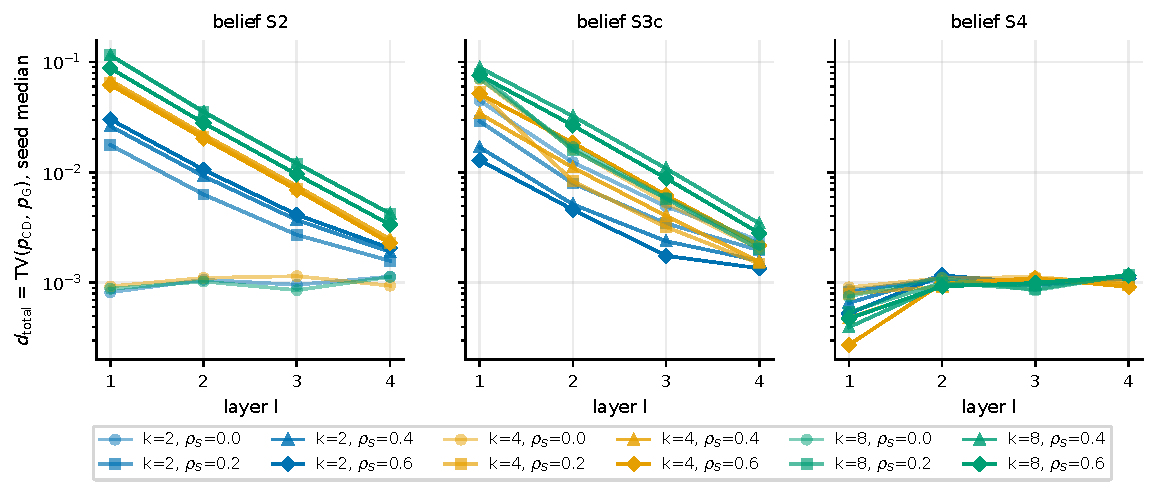
\includegraphics[width=0.9\linewidth]{G8_depth.pdf}
\caption{$\dtot$ by layer for chains with direct estimates: seed medians over 10 seeds, neuron 1 in the pair basis, $m=4$, $n=10^6$, for $k\in\{2,4,8\}$ and $\rs\in\{0,0.2,0.4,0.6\}$. The decline under S2 and S3c reflects the target approaching the uniform density, not improved accuracy. Values near $10^{-3}$ are at Monte Carlo noise level.}
\label{fig:depth}
\end{figure}

\begin{figure}[ht]
\centering
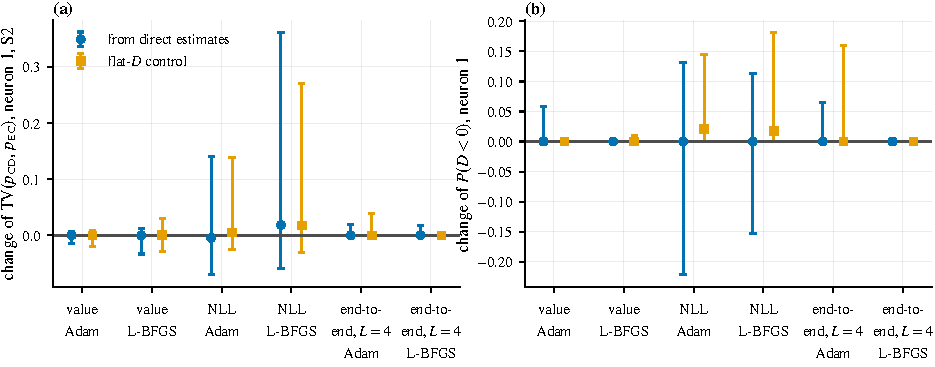
\includegraphics[width=0.78\linewidth]{G9_training.pdf}
\caption{Effect of training on neuron 1 under S2. Left: change of $\ddc=\TV(\pcd,\pec)$, shown because it exists everywhere; this is not the pre-registered $\dden$ of H5b. Right: change of $P(D<0)$. Points are medians and bars $10$--$90\,\%$ ranges over all $k$, $\rs$, bases and seeds, from direct estimates and from the flat-$D$ control. Runs labelled e2e are the $L=4$ runs.}
\label{fig:train}
\end{figure}

\clearpage
\section{Additional tables and figures}\label{app:thr}

\begin{table}[ht]
\centering
\small
\begin{tabular}{lrrrrrr}
\toprule
type, basis & points & $\beta$ (H1c) & power law & closed form & ratio range & median ratio \\
\midrule
SUM, pair & 33 & 1.76 & 55\,\% & 100\,\% & 0.61--1.65 & 0.88 \\
CONTRAST, pair & 33 & 1.59 & 52\,\% & 100\,\% & 0.61--1.65 & 0.87 \\
SUM, triple & 23 & 0.88 & 100\,\% & 100\,\% & 0.57--0.99 & 0.79 \\
CONTRAST, triple & 23 & 1.00 & 48\,\% & 100\,\% & 1.00--1.76 & 1.07 \\
\bottomrule
\end{tabular}

\caption{H1c points against the frozen power law and the closed forms (post hoc). ``power law'' and ``closed form'' give the share of points within a factor 2 of the fit and of the formula; ``ratio'' is measured $\dden$ over the formula.}
\label{tab:lead}
\end{table}

\begin{table}[ht]
\centering
\small
\begin{tabular}{lrrrrrr}
\toprule
basis & $k$ & $d_{\mathrm{denom}}\geq 1\,\%$ & $d_{\mathrm{denom}}\geq 5\,\%$ & onset, $n=10^7$ & onset, pop. & undefined from \\
\midrule
pair & 2 & 0.192 & 0.359 & 0.435 & 0.437 & 0.450 \\
pair & 4 & 0.102 & --- & 0.201 & 0.204 & 0.200 \\
pair & 8 & 0.067 & --- & 0.123 & 0.129 & 0.150 \\
pair & 16 & 0.043 & --- & 0.059 & 0.074 & 0.075 \\
pair & 32 & --- & --- & 0.007 & 0.039 & 0.010 \\
triple & 2 & 0.085 & --- & 0.435 & 0.437 & 0.450 \\
triple & 4 & 0.020 & --- & 0.085 & 0.094 & 0.100 \\
triple & 8 & 0.009 & --- & 0.016 & 0.045 & 0.020 \\
triple & 16 & --- & --- & 0.000 & 0.023 & 0.000 \\
triple & 32 & --- & --- & 0.000 & 0.011 & 0.000 \\
\bottomrule
\end{tabular}

\caption{Thresholds in $\rs$ for type SUM, flat belief S2, $m=4$, seed-median curves, $n=10^7$ except the population onset. ``---'' means the level was not reached before $\peu$ became undefined; it never means that the error is small. ``undefined from'' is the first grid value at which most seeds have $\peu$ undefined. Onsets are upper bounds. CONTRAST and all confidence intervals are in Table~\ref{tab:thrfull}.}
\label{tab:thr}
\end{table}

\begin{table}[ht]
\centering
\footnotesize
\begin{tabular}{rrrrrrrr}
\toprule
& & \multicolumn{2}{c}{evidence} & \multicolumn{2}{c}{posterior} & \multicolumn{2}{c}{marginal} \\ \cmidrule(lr){3-4}\cmidrule(lr){5-6}\cmidrule(l){7-8}
$\rho_S$ & $\sigma_{\mathrm{obs}}$ & CD & EU & CD & EU & CD & EU \\
\midrule
0.1 & 0.5 & 0.013 & 0.013 & 0.014 & 0.013 & 0.014 & 0.013 \\
 & 1.0 & 0.008 & 0.010 & 0.011 & 0.008 & 0.010 & 0.009 \\
0.2 & 0.5 & 0.011 & 0.013 & 0.014 & 0.011 & 0.014 & 0.012 \\
 & 1.0 & 0.008 & 0.015 & 0.017 & 0.008 & 0.015 & 0.009 \\
0.3 & 0.5 & 0.011 & 0.016 & 0.015 & 0.011 & 0.014 & 0.011 \\
 & 1.0 & 0.008 & 0.024 & 0.030 & 0.008 & 0.023 & 0.009 \\
0.4 & 0.5 & 0.010 & 0.016 & 0.015 & 0.010 & 0.014 & 0.010 \\
 & 1.0 & 0.008 & 0.028 & 0.034 & 0.008 & 0.024 & 0.010 \\
\bottomrule
\end{tabular}

\caption{Illustration at $k=2$ (Section~\ref{sec:illus}): median TV to the truth over 200 observations. Not a study result.}
\label{tab:sem}
\end{table}

\begin{table}[ht]
\centering
\scriptsize\setlength{\tabcolsep}{3.5pt}
\begin{tabular}{rrrrrrrrrrrr}
\toprule
$k$ & $\rho_S$ & $\tau$ & evid.\ CD & EU & CD closer & post.\ CD & EU & CD closer & marg.\ CD & EU & CD closer \\
\midrule
4 & 0.10 & 0.5 & 0.131 & 0.133 & 93\,\% & 0.131 & 0.132 & 88\,\% & 0.133 & 0.133 & 88\,\% \\
4 & 0.10 & 1.0 & 0.078 & 0.092 & 93\,\% & 0.075 & 0.081 & 73\,\% & 0.080 & 0.088 & 75\,\% \\
4 & 0.15 & 0.5 & 0.132 & 0.136 & 90\,\% & 0.129 & 0.132 & 85\,\% & 0.133 & 0.132 & 83\,\% \\
4 & 0.15 & 1.0 & 0.072 & 0.078 & 92\,\% & 0.074 & 0.073 & 53\,\% & 0.088 & 0.089 & 63\,\% \\
8 & 0.05 & 0.5 & 0.139 & 0.141 & 73\,\% & 0.139 & 0.139 & 63\,\% & 0.142 & 0.143 & 68\,\% \\
8 & 0.05 & 1.0 & 0.073 & 0.081 & 88\,\% & 0.073 & 0.074 & 67\,\% & 0.082 & 0.083 & 68\,\% \\
8 & 0.10 & 0.5 & 0.186 & 0.187 & 63\,\% & 0.181 & 0.178 & 60\,\% & 0.173 & 0.176 & 63\,\% \\
8 & 0.10 & 1.0 & 0.099 & 0.113 & 67\,\% & 0.092 & 0.101 & 55\,\% & 0.119 & 0.124 & 48\,\% \\
\bottomrule
\end{tabular}

\caption{Illustration at $k=4,8$, pair basis, below the onset, 60 observations; ``CD closer'' is the share of observations with $\pcd$ nearer the truth than $\peu$. Truncation hides the flip of Table~\ref{tab:sem}. Not a study result.}
\label{tab:sembig}
\end{table}

\begin{table}[ht]
\centering
\footnotesize
\begin{tabular}{llrrrrrr}
\toprule
basis & belief & evaluations & share undefined & $d_{\mathrm{total}}$ & $d_{\mathrm{dc}}$ & $d_{\mathrm{model,cal}}$ & CD closer than EC \\
\midrule
pair & S2 & 6{,}098 & 68\,\% & 0.098 & 0.086 & 0.146 & 64\,\% \\
 & S3a & 3{,}963 & 44\,\% & 0.054 & 0.008 & 0.050 & 30\,\% \\
 & S3b & 2{,}800 & 31\,\% & 0.067 & 0.011 & 0.057 & 25\,\% \\
 & S3c & 5{,}751 & 64\,\% & 0.067 & 0.052 & 0.086 & 64\,\% \\
 & S3d & 1{,}978 & 22\,\% & 0.046 & 0.001 & 0.041 & 25\,\% \\
 & S4 & 6{,}098 & 68\,\% & 0.000 & 0.017 & 0.017 & 97\,\% \\
\midrule
triple & S2 & 7{,}196 & 80\,\% & 0.079 & 0.051 & 0.068 & 41\,\% \\
 & S3a & 5{,}845 & 65\,\% & 0.078 & 0.042 & 0.073 & 50\,\% \\
 & S3b & 5{,}663 & 63\,\% & 0.112 & 0.053 & 0.086 & 38\,\% \\
 & S3c & 6{,}949 & 77\,\% & 0.033 & 0.053 & 0.061 & 71\,\% \\
 & S3d & 4{,}601 & 51\,\% & 0.102 & 0.036 & 0.105 & 54\,\% \\
 & S4 & 7{,}196 & 80\,\% & 0.022 & 0.039 & 0.021 & 54\,\% \\
\bottomrule
\end{tabular}

\caption{Past the onset: rows with $\peu$ undefined, $\rs>0$, $m=4$, $\varepsilon=0.01$, medians (post hoc). ``CD closer than EC'': share of rows with $\pcd$ nearer to $\pg$ than $\pec$. Here truth is the Jeffrey answer.}
\label{tab:past}
\end{table}

\begin{table}[ht]
\centering
\footnotesize
\begin{tabular}{rrrrrrrrr}
\toprule
& & \multicolumn{5}{c}{pair} & \multicolumn{2}{c}{triple} \\ \cmidrule(lr){3-7}\cmidrule(l){8-9}
$m$ & $k$ & first & convex & search & measured & $k\rho_S^\ast$ & corner & measured \\
\midrule
2 & 2 & 0.247 & 0.406 & 0.545 & 0.545 & 1.09 & --- & --- \\
 & 4 & 0.140 & 0.261 & 0.261 & 0.261 & 1.04 & --- & 0.199 \\
 & 8 & 0.075 & 0.158 & 0.158 & 0.158 & 1.26 & --- & 0.087 \\
 & 16 & 0.039 & 0.090 & 0.090 & 0.090 & 1.44 & --- & 0.041 \\
 & 32 & 0.020 & 0.049 & 0.049 & 0.049 & 1.57 & --- & 0.021 \\
\midrule
4 & 2 & 0.152 & 0.289 & 0.437 & 0.437 & 0.87 & --- & --- \\
 & 4 & 0.085 & 0.201 & 0.204 & 0.204 & 0.82 & 0.093 & 0.094 \\
 & 8 & 0.046 & 0.127 & 0.129 & 0.129 & 1.03 & 0.044 & 0.045 \\
 & 16 & 0.024 & 0.073 & 0.074 & 0.074 & 1.18 & 0.022 & 0.023 \\
 & 32 & 0.012 & 0.039 & 0.039 & 0.039 & 1.26 & 0.012 & 0.011 \\
\midrule
6 & 2 & 0.120 & 0.229 & 0.398 & 0.398 & 0.80 & --- & --- \\
 & 4 & 0.068 & 0.167 & 0.168 & 0.168 & 0.67 & 0.070 & 0.070 \\
 & 8 & 0.036 & 0.111 & 0.116 & 0.116 & 0.92 & 0.033 & 0.035 \\
 & 16 & 0.019 & 0.068 & 0.068 & 0.068 & 1.09 & 0.017 & 0.018 \\
 & 32 & 0.010 & 0.038 & 0.038 & 0.038 & 1.21 & 0.009 & 0.009 \\
\bottomrule
\end{tabular}

\caption{Onsets for all degrees (population, SUM, S2, post hoc for the bounds). ``search'': best upper value found by coordinate descent, capped by ``measured''. ``---'': no corner goes negative, or $k=2$, where the triple family equals the pair family for $D$.}
\label{tab:onsetall}
\end{table}

\begin{table}[ht]
\centering
\footnotesize
\begin{tabular}{lrrrrrr}
\toprule
basis & $k$ & $z$ production & $z$ corners & $z$ cube & coordinates on the boundary & $\sqrt{2k\ln 2}$ \\
\midrule
pair & 2 & 1.0 & 1.2 & 1.2 & 100\,\% & 1.7 \\
pair & 4 & 1.8 & 1.5 & 1.7 & 75\,\% & 2.4 \\
pair & 8 & 2.5 & 2.0 & 2.4 & 75\,\% & 3.3 \\
pair & 16 & 3.5 & 2.9 & 3.8 & 75\,\% & 4.7 \\
pair & 32 & 4.4 & 4.4 & 5.5 & 77\,\% & 6.7 \\
triple & 4 & 1.8 & 1.5 & 1.8 & 100\,\% & 2.4 \\
triple & 8 & 2.6 & 2.4 & 2.7 & 88\,\% & 3.3 \\
triple & 16 & 3.3 & 3.7 & 3.7 & 91\,\% & 4.7 \\
\bottomrule
\end{tabular}

\caption{$z=(1-\min D)/\sigma_{\mathrm c}$ at $\rs=0$, $m=4$ (post hoc). ``production'' from $n=10^7$. ``corners'' and ``cube'': Gaussian surrogate of Proposition~\ref{prop:noise} by coordinate descent, medians over a few draws. ``coordinates on the boundary'': share in the cube minimiser.}
\label{tab:noisez}
\end{table}

\begin{table}[ht]
\centering
\footnotesize
\begin{tabular}{lrrrrrrr}
\toprule
basis & $k$ & $|B_D|$ & $\sigma_{\mathrm{c}}$ & $1-\min D$ & ratio & $\chi_D$ & $\sqrt{|B_D|/n}$ \\
\midrule
pair & 2 & 24 & 0.008 & 0.008 & 1.0 & \ensuremath{1.52\times 10^{-3}} & \ensuremath{1.55\times 10^{-3}} \\
 & 4 & 112 & 0.019 & 0.035 & 1.8 & \ensuremath{3.32\times 10^{-3}} & \ensuremath{3.35\times 10^{-3}} \\
 & 8 & 480 & 0.040 & 0.099 & 2.5 & \ensuremath{6.87\times 10^{-3}} & \ensuremath{6.93\times 10^{-3}} \\
 & 16 & 1{,}984 & 0.083 & 0.292 & 3.5 & \ensuremath{1.41\times 10^{-2}} & \ensuremath{1.41\times 10^{-2}} \\
 & 32 & 8{,}064 & 0.169 & 0.746 & 4.4 & \ensuremath{2.84\times 10^{-2}} & \ensuremath{2.84\times 10^{-2}} \\
triple & 4 & 368 & 0.077 & 0.134 & 1.8 & \ensuremath{5.99\times 10^{-3}} & \ensuremath{6.07\times 10^{-3}} \\
 & 8 & 4{,}064 & 0.281 & 0.734 & 2.6 & \ensuremath{2.01\times 10^{-2}} & \ensuremath{2.02\times 10^{-2}} \\
 & 16 & 37{,}824 & 0.884 & 2.948 & 3.3 & \ensuremath{6.15\times 10^{-2}} & \ensuremath{6.15\times 10^{-2}} \\
 & 32 & 325{,}504 & 2.624 & 11.066 & 4.2 & \ensuremath{1.80\times 10^{-1}} & \ensuremath{1.80\times 10^{-1}} \\
\bottomrule
\end{tabular}

\caption{Noise scale at $\rs=0$, $m=4$, $n=10^7$, type SUM, S2 (post hoc). $\sigma_{\mathrm c}=\sqrt{K_{\mathrm c}/n}$ from Proposition~\ref{prop:noise}; ``ratio'' is $(1-\min D)/\sigma_{\mathrm c}$. The triple basis at $k=2$ is omitted because it equals the pair basis for $D$.}
\label{tab:noise}
\end{table}

\begin{table}[ht]
\centering
\scriptsize\setlength{\tabcolsep}{4pt}
\begin{tabular}{llrlllrr}
\toprule
type & basis & $k$ & $d_{\mathrm{denom}}\geq 1\,\%$ & $d_{\mathrm{denom}}\geq 5\,\%$ & onset, $n=10^7$ & onset, pop. & undefined from \\
\midrule
SUM & pair & 2 & 0.192 (0.192--0.193) & 0.359 (0.359--0.360) & 0.435 (0.435--0.436) & 0.437 & 0.450 \\
SUM & pair & 4 & 0.102 (0.101--0.102) & --- & 0.201 (0.201--0.201) & 0.204 & 0.200 \\
SUM & pair & 8 & 0.067 (0.067--0.067) & --- & 0.123 (0.123--0.123) & 0.129 & 0.150 \\
SUM & pair & 16 & 0.043 (0.043--0.043) & --- & 0.059 (0.059--0.060) & 0.074 & 0.075 \\
SUM & pair & 32 & --- & --- & 0.007 (0.007--0.008) & 0.039 & 0.010 \\
SUM & triple & 2 & 0.085 (0.085--0.086) & --- & 0.435 (0.435--0.436) & 0.437 & 0.450 \\
SUM & triple & 4 & 0.020 (0.020--0.020) & --- & 0.085 (0.083--0.087) & 0.094 & 0.100 \\
SUM & triple & 8 & 0.009 (0.009--0.009) & --- & 0.016 (0.015--0.017) & 0.045 & 0.020 \\
SUM & triple & 16 & --- & --- & 0.000 (0.000--0.000) & 0.023 & 0.000 \\
SUM & triple & 32 & --- & --- & 0.000 (0.000--0.000) & 0.011 & 0.000 \\
\midrule
CONTRAST & pair & 2 & 0.192 (0.192--0.192) & 0.388 (0.387--0.388) & 0.435 (0.435--0.435) & 0.437 & 0.450 \\
CONTRAST & pair & 4 & 0.122 (0.121--0.122) & --- & 0.201 (0.201--0.201) & 0.204 & 0.200 \\
CONTRAST & pair & 8 & 0.084 (0.084--0.084) & --- & 0.123 (0.123--0.123) & 0.129 & 0.150 \\
CONTRAST & pair & 16 & --- & --- & 0.059 (0.059--0.060) & 0.074 & 0.075 \\
CONTRAST & pair & 32 & --- & --- & 0.007 (0.007--0.008) & 0.039 & 0.010 \\
CONTRAST & triple & 2 & 0.065 (0.065--0.065) & 0.235 (0.235--0.235) & 0.435 (0.435--0.435) & 0.437 & 0.450 \\
CONTRAST & triple & 4 & 0.054 (0.054--0.054) & --- & 0.084 (0.082--0.086) & 0.094 & 0.100 \\
CONTRAST & triple & 8 & --- & --- & 0.015 (0.013--0.018) & 0.045 & 0.020 \\
CONTRAST & triple & 16 & --- & --- & 0.000 (0.000--0.000) & 0.023 & 0.000 \\
CONTRAST & triple & 32 & --- & --- & 0.000 (0.000--0.000) & 0.011 & 0.000 \\
\bottomrule
\end{tabular}

\caption{All thresholds for S2, $m=4$, with $95\,\%$ bootstrap CIs. ``---'' as in Table~\ref{tab:thr}.}
\label{tab:thrfull}
\end{table}

\begin{table}[ht]
\centering
\footnotesize
\begin{tabular}{llrllr}
\toprule
type & basis & $k$ & $|\mathrm{relvar}|\geq 5\,\%$ & $|\mathrm{relvar}|\geq 20\,\%$ & $\min D$ at $\rho_S=0$ \\
\midrule
SUM & pair & 2 & 0.283 (0.282--0.283) & --- & 0.992 \\
SUM & pair & 4 & 0.147 (0.146--0.147) & --- & 0.965 \\
SUM & pair & 8 & 0.095 (0.095--0.095) & --- & 0.901 \\
SUM & pair & 16 & --- & --- & 0.708 \\
SUM & pair & 32 & --- & --- & 0.254 \\
SUM & triple & 2 & 0.246 (0.245--0.246) & --- & 0.992 \\
SUM & triple & 4 & 0.048 (0.048--0.048) & --- & 0.866 \\
SUM & triple & 8 & --- & --- & 0.266 \\
SUM & triple & 16 & --- & --- & -1.948 \\
SUM & triple & 32 & --- & --- & -10.066 \\
CONTRAST & pair & 2 & 0.299 (0.299--0.299) & --- & 0.992 \\
CONTRAST & pair & 4 & --- & --- & 0.966 \\
CONTRAST & pair & 8 & --- & --- & 0.895 \\
CONTRAST & pair & 16 & --- & --- & 0.711 \\
CONTRAST & pair & 32 & --- & --- & 0.253 \\
CONTRAST & triple & 2 & 0.139 (0.139--0.139) & --- & 0.992 \\
CONTRAST & triple & 4 & --- & --- & 0.863 \\
CONTRAST & triple & 8 & --- & --- & 0.250 \\
CONTRAST & triple & 16 & --- & --- & -2.068 \\
CONTRAST & triple & 32 & --- & --- & -10.202 \\
\bottomrule
\end{tabular}

\caption{Thresholds of the relative variance error (S2, $m=4$) and $\min D$ at $\rs=0$. ``---'' as in Table~\ref{tab:thr}.}
\label{tab:relvar}
\end{table}

\begin{table}[ht]
\centering
\footnotesize
\begin{tabular}{lrllllll}
\toprule
type & $k$ & S2 & S3a & S3b & S3c & S3d & S4 \\
\midrule
SUM & 2 & 0.192 / 0.45 & --- / 0.45 & --- / 0.45 & 0.217 / 0.45 & --- / 0.60 & --- / 0.45 \\
 & 4 & 0.102 / 0.20 & --- / 0.25 & 0.039 / 0.25 & 0.125 / 0.20 & --- / 0.35 & --- / 0.20 \\
 & 8 & 0.067 / 0.15 & --- / 0.15 & 0.014 / 0.20 & --- / 0.15 & --- / 0.35 & --- / 0.15 \\
 & 16 & 0.043 / 0.075 & --- / 0.15 & 0.009 / 0.90 & --- / 0.075 & --- / --- & --- / 0.075 \\
 & 32 & --- / 0.010 & 0.054 / --- & 0.027 / --- & --- / 0.050 & --- / --- & --- / 0.010 \\
\midrule
CONTRAST & 2 & 0.192 / 0.45 & --- / 0.45 & --- / 0.45 & 0.102 / 0.45 & --- / 0.60 & --- / 0.45 \\
 & 4 & 0.122 / 0.20 & --- / 0.25 & --- / 0.25 & 0.177 / 0.25 & --- / 0.35 & --- / 0.20 \\
 & 8 & 0.084 / 0.15 & --- / 0.15 & --- / 0.20 & --- / 0.15 & --- / 0.35 & --- / 0.15 \\
 & 16 & --- / 0.075 & --- / 0.15 & --- / 0.90 & --- / 0.075 & --- / --- & --- / 0.075 \\
 & 32 & --- / 0.010 & --- / --- & --- / --- & --- / 0.050 & --- / --- & --- / 0.010 \\
\bottomrule
\end{tabular}

\caption{$1\,\%$ threshold of $\dden$ and undefined onset (shown as threshold / onset) for all beliefs, pair basis, $m=4$. ``---'' in the onset means $\peu$ stayed defined up to $\rs=0.9$; only then does ``---'' in the threshold mean that the level was not reached in the range.}
\label{tab:bel}
\end{table}

\begin{table}[ht]
\centering
\footnotesize
\begin{tabular}{llrrrrrr}
\toprule
belief & type & $\rho_S$ & $d_{\mathrm{denom}}$ & $d_{\mathrm{neg}}$ & $d_{\mathrm{model,uncal}}$ & $d_{\mathrm{model,cal}}$ & $d_{\mathrm{total}}$ \\
\midrule
S2 & SUM & 0.1 & 0.0025 & 0.0111 & 0.0131 & 0.0241 & 0.0106 \\
 &  & 0.2 & 0.0108 & 0.0076 & 0.0287 & 0.0358 & 0.0180 \\
 &  & 0.4 & 0.0736 & 0.0376 & 0.1002 & 0.0627 & 0.0265 \\
 & CONTRAST & 0.1 & 0.0025 & 0.0123 & 0.0129 & 0.0026 & 0.0154 \\
 &  & 0.2 & 0.0108 & 0.0095 & 0.0267 & 0.0195 & 0.0374 \\
 &  & 0.4 & 0.0547 & 0.0238 & 0.0397 & 0.0617 & 0.0906 \\
\midrule
S3c & SUM & 0.1 & 0.0034 & 0.0064 & 0.0399 & 0.0445 & 0.0368 \\
 &  & 0.2 & 0.0087 & 0.0064 & 0.0372 & 0.0415 & 0.0294 \\
 &  & 0.4 & 0.0355 & 0.0061 & 0.0485 & 0.0438 & 0.0171 \\
 & CONTRAST & 0.1 & 0.0097 & 0.0391 & 0.0650 & 0.0673 & 0.0710 \\
 &  & 0.2 & 0.0262 & 0.0551 & 0.0854 & 0.0971 & 0.1022 \\
 &  & 0.4 & 0.1030 & 0.1116 & 0.0985 & 0.1371 & 0.1526 \\
\midrule
S4 & SUM & 0.1 & 0.0001 & 0.0120 & 0.0003 & 0.0119 & 0.0003 \\
 &  & 0.2 & 0.0004 & 0.0103 & 0.0004 & 0.0100 & 0.0003 \\
 &  & 0.4 & 0.0003 & 0.0037 & 0.0004 & 0.0037 & 0.0002 \\
 & CONTRAST & 0.1 & 0.0001 & 0.0118 & 0.0003 & 0.0118 & 0.0003 \\
 &  & 0.2 & 0.0004 & 0.0104 & 0.0004 & 0.0101 & 0.0003 \\
 &  & 0.4 & 0.0003 & 0.0044 & 0.0004 & 0.0045 & 0.0004 \\
\bottomrule
\end{tabular}

\caption{Error components at $k=2$, pair basis, $m=4$, $n=10^7$, $\varepsilon=0.01$, seed medians.}
\label{tab:decomp}
\end{table}

\begin{figure}[ht]
\centering
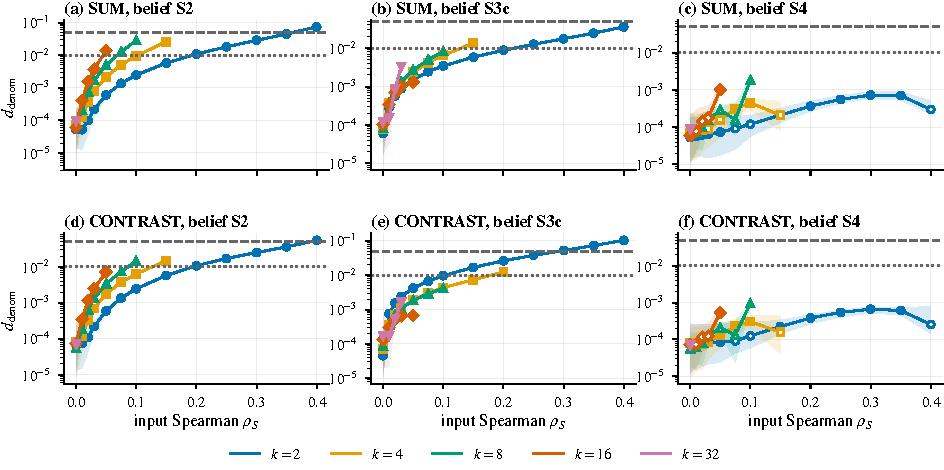
\includegraphics[width=0.92\linewidth]{G1_d_denom_vs_rho.pdf}
\caption{$\dden$ against input Spearman correlation $\rs$ for the pair basis, $m=4$, $n=10^7$, $\varepsilon=0.01$, beliefs S2, S3c and S4. Lines are seed medians and bands $2.5$--$97.5\,\%$ seed intervals. A curve ends where most seeds have $\peu$ undefined; the gap carries no information about the error. Hollow markers are below three times the Monte Carlo noise floor. Dotted and dashed lines mark $1\,\%$ and $5\,\%$.}
\label{fig:d}
\end{figure}

\begin{figure}[ht]
\centering
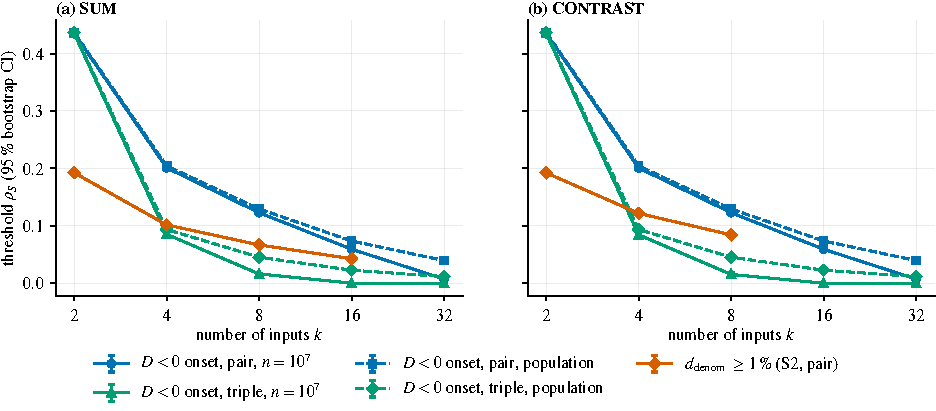
\includegraphics[width=0.76\linewidth]{G2_thresholds_vs_k.pdf}
\caption{Negativity onsets for both bases, at $n=10^7$ (solid) and with population coefficients (dashed), and the $1\,\%$ threshold of $\dden$ (S2, pair), against $k$, for $m=4$. Error bars are $95\,\%$ bootstrap CIs and are often smaller than the markers. Missing points mean the level was not reached before $\peu$ became undefined.}
\label{fig:thr}
\end{figure}

\begin{figure}[ht]
\centering
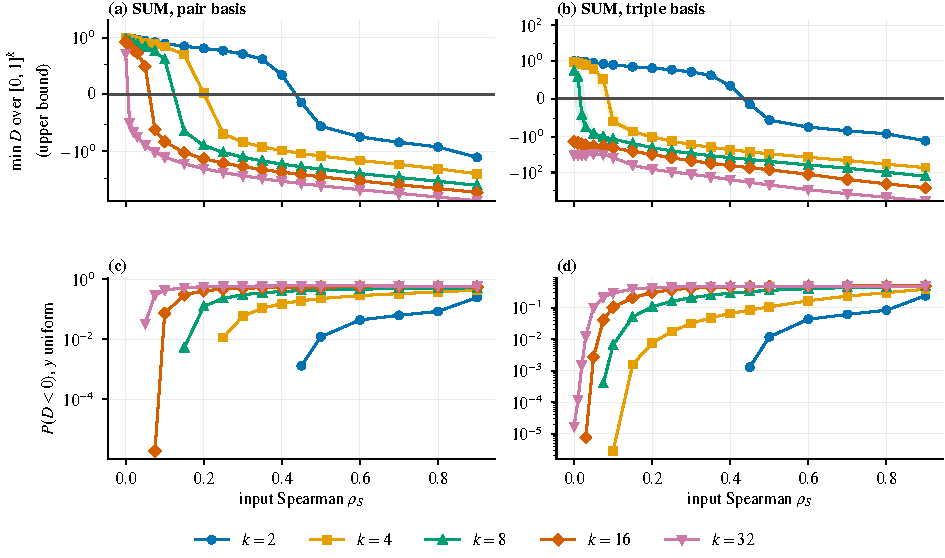
\includegraphics[width=0.68\linewidth]{G3_negativity.pdf}
\caption{Negativity of $D$ for type SUM, $m=4$, $n=10^7$, seed medians. Top: $\min D$ over $[0,1]^k$ on a symmetric logarithmic axis; the value is an upper bound on the true minimum. Bottom: $P(D<0)$ under uniform $y$ on a logarithmic axis; points with zero observed probability are not drawn.}
\label{fig:neg}
\end{figure}

\begin{figure}[ht]
\centering
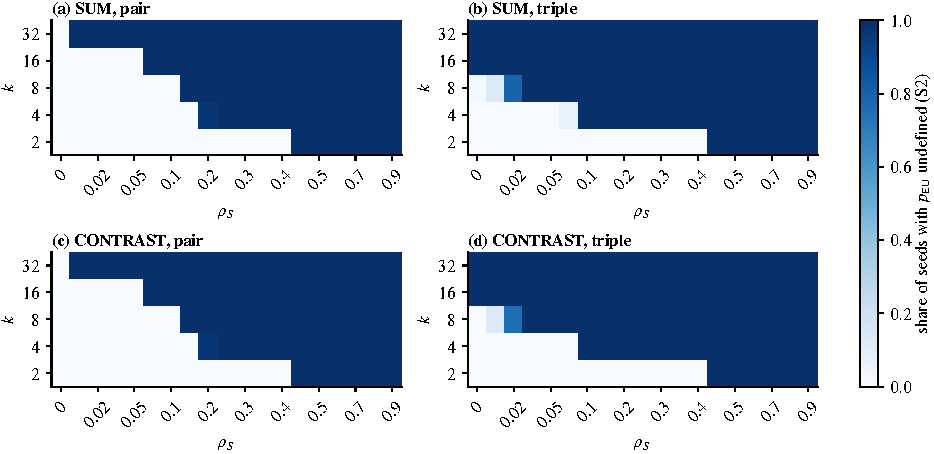
\includegraphics[width=0.9\linewidth]{G4_undefined_share.pdf}
\caption{Share of seeds with $\peu$ undefined under S2, $m=4$, $n=10^7$. The $\rs$ axis is categorical (grid values, unevenly spaced). Dark regions are where $\dden$ cannot be measured.}
\label{fig:undef}
\end{figure}

\begin{figure}[ht]
\centering
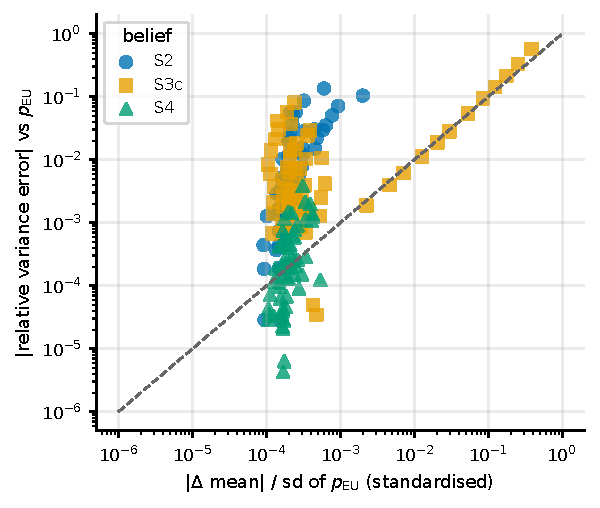
\includegraphics[width=0.5\linewidth]{G6_mean_vs_variance.pdf}
\caption{Absolute relative variance error against standardised mean error, both relative to $\peu$, pair basis, $m=4$, $\varepsilon=0.01$, all $k$, types and $\rs>0$ where defined; seed medians. Points above the dashed line have larger variance error than mean error.}
\label{fig:mv}
\end{figure}

\begin{figure}[ht]
\centering
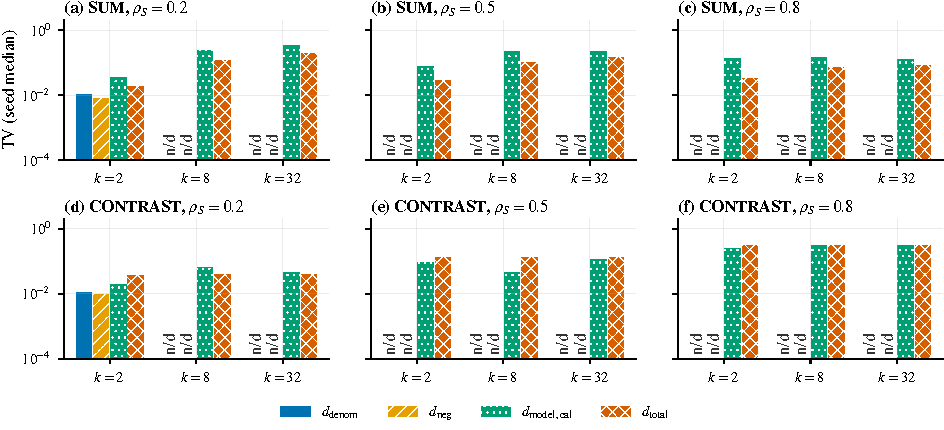
\includegraphics[width=0.74\linewidth]{G7_decomposition.pdf}
\caption{Error components under the flat belief S2, pair basis, $m=4$, $n=10^7$, $\varepsilon=0.01$; seed medians at three correlations and three values of $k$. ``n/d'' marks quantities not defined because $\peu$ is undefined, not values near zero. $\dtot$ under S2 is dominated by the mismatch between the flat belief and the truth.}
\label{fig:dec}
\end{figure}

\FloatBarrier
\section{Hypothesis details}\label{app:hyp}

Decision rules are quoted in substance from Section~6 of the pre-registration.
H1a, H2a, H2b (population): deterministic inequality per cell. H1b, H2b ($n=10^7$), H5a--d: aggregation rule of Section~\ref{sec:design}. H1c: power law per (type, basis), $\geq90\,\%$ of points within a factor 2 for \emph{supported}, $<50\,\%$ for \emph{not supported}. H2c: $\max/\min$ over $m$ at most $1.5$ at $\geq80\,\%$ of points for \emph{supported}, $\leq50\,\%$ for \emph{not supported}. H3a: \emph{supported} if every CI is inside $[-0.05,0.05]$, \emph{not supported} if any is entirely outside. H3b: same with the ratio in $[0.5,2]$. H3c: $\geq80\,\%$ for \emph{supported}, $<50\,\%$ for \emph{not supported}. H4a: $\geq90\,\%$ for \emph{supported}, $<50\,\%$ for \emph{not supported}. H4b: every violation is listed in \texttt{results2/summary/convergence\_violations.csv}. The two bases coincide for $D$ at $k=2$, which is why $k=2$ is not in H2b.

\begin{table}[ht]
\centering
\footnotesize
\begin{tabular}{llrrrrl}
\toprule
type & basis & points & $\beta$ & $C$ & within $2\times$ & cell verdict \\
\midrule
CONTRAST & pair & 33 & 1.59 & 0.040 & 0.52 & inconclusive \\
CONTRAST & triple & 23 & 1.00 & 0.083 & 0.48 & not supported \\
SUM & pair & 33 & 1.76 & 0.070 & 0.55 & inconclusive \\
SUM & triple & 23 & 0.88 & 0.107 & 1.00 & supported \\
\bottomrule
\end{tabular}

\caption{H1c fits $\dden=C\chi_D^\beta$ on population coefficients, S2, $m=4$. Cell verdicts follow the H1c rule.}
\label{tab:h1c}
\end{table}

\begin{table}[ht]
\centering
\footnotesize
\begin{tabular}{rrrrrrr}
\toprule
& \multicolumn{3}{c}{pair} & \multicolumn{3}{c}{triple} \\ \cmidrule(lr){2-4}\cmidrule(l){5-7}
$k$ & $m=2$ & $m=4$ & $m=6$ & $m=2$ & $m=4$ & $m=6$ \\
\midrule
2 & 0.545 & 0.437 & 0.398 & 0.545 & 0.437 & 0.398 \\
4 & 0.261 & 0.204 & 0.168 & 0.199 & 0.094 & 0.070 \\
8 & 0.158 & 0.129 & 0.116 & 0.087 & 0.045 & 0.035 \\
16 & 0.090 & 0.074 & 0.068 & 0.041 & 0.023 & 0.018 \\
32 & 0.049 & 0.039 & 0.038 & 0.021 & 0.011 & 0.009 \\
\bottomrule
\end{tabular}

\caption{Population negativity onset by degree (H2a), type SUM.}
\label{tab:onsetm}
\end{table}

\begin{table}[ht]
\centering
\small
\begin{tabular}{lrcrrr}
\toprule
family & cells & onset $-$ Gaussian (min \dots\ max) & CI inside & CI outside & median ratio \\
\midrule
clayton & 6 & -0.179 \dots\ +0.006 & 2 & 4 & 5.34 \\
gumbel & 6 & -0.128 \dots\ -0.013 & 1 & 5 & 16.60 \\
t10 & 18 & -0.102 \dots\ +0.036 & 15 & 3 & 2.08 \\
t3 & 18 & -0.201 \dots\ -0.016 & 3 & 15 & 7.22 \\
\bottomrule
\end{tabular}

\caption{Comparison with the Gaussian copula at matched Kendall's $\tau$ ($m=4$, pair and triple, $k\in\{2,4,8\}$, $n=10^7$, 20 seeds). Columns: range of onset differences; number of 95\,\% CIs inside and entirely outside $\pm0.05$; median ratio of $\dden$ to Gaussian under S2.}
\label{tab:fam}
\end{table}

\begin{figure}[ht]
\centering
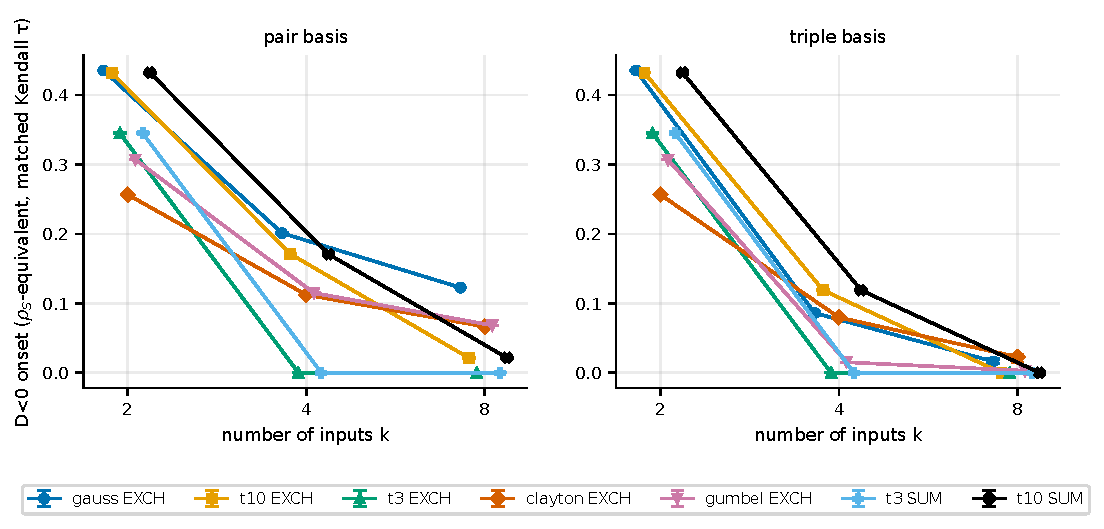
\includegraphics[width=0.8\linewidth]{G5_copula_families.pdf}
\caption{Negativity onset by copula family at matched Kendall's $\tau$, expressed in $\rs$ units, $m=4$, $n=10^7$, 20 seeds, with $95\,\%$ bootstrap CIs (mostly smaller than the markers). Points are shifted slightly in $k$ for legibility. EXCH families and the $t$ SUM forms are shown; $t$ CONTRAST is in Table~\ref{tab:fam}. An onset of $0$ means $\min D<0$ at $\rs=0$.}
\label{fig:fam}
\end{figure}

\begin{table}[ht]
\centering
\footnotesize
\begin{tabular}{rrrrrr}
\toprule
$k$ & $\eta$ & defined & drawn & within $2\times$, pair & within $2\times$, triple \\
\midrule
2 & 1 & 108 & 200 & 38\,\% & 49\,\% \\
2 & 4 & 165 & 200 & 39\,\% & 24\,\% \\
\bottomrule
\end{tabular}

\caption{H3c by $k$ and $\eta$. ``defined'' counts matrices with $\peu$ defined (pair basis, S2, $m=4$). Shares are among defined matrices. The rule is at least $80\,\%$ for \emph{supported} and below $50\,\%$ for \emph{not supported}.}
\label{tab:lkj}
\end{table}

\begin{table}[ht]
\centering
\footnotesize
\begin{tabular}{lrrrrD{.}{.}{2}}
\toprule
variant & paired values & violations & median change & max change & \multicolumn{1}{c}{worst ratio} \\
\midrule
$M\times 2$ & 291{,}249 & 0 & \ensuremath{1.9\times 10^{-5}} & \ensuremath{4.6\times 10^{-1}} & 0.86 \\
$n\times 2$ & 291{,}258 & 5{,}460 & \ensuremath{4.6\times 10^{-5}} & \ensuremath{8.3\times 10^{0}} & 36.21 \\
$s$-nodes $\times 2$ & 291{,}276 & 0 & \ensuremath{2.7\times 10^{-9}} & \ensuremath{3.7\times 10^{-5}} & 0.00 \\
$x$-nodes $\times 2$ & 291{,}276 & 0 & \ensuremath{4.0\times 10^{-10}} & \ensuremath{6.4\times 10^{-6}} & 0.00 \\
\bottomrule
\end{tabular}

\caption{Convergence test H4b on the \texttt{convergence} subset ($k\in\{2,8,32\}$, 5 seeds). Paired values are reported TVs before and after doubling one setting; a violation is a change of at least $\max(3\,\mathrm{SE},10^{-3})$. The final column is the largest ratio of change to tolerance.}
\label{tab:conv}
\end{table}

\FloatBarrier
\section{Numerics}\label{app:numerics}

$\min D$ uses \V{cfg.starts} starts (corners, edge midpoints, the 256 lowest-$D$ Monte Carlo samples of S2 and S4, and uniform random points), projected Adam for 400 steps, cosine learning rate from $0.005$ to $0.0001$, projected onto the support for Beta beliefs, and takes the minimum with the Monte Carlo minimum. These settings were chosen on $d=3$ coefficients against brute-force grids, not on production data. Random numbers come from PCG64 with \texttt{SeedSequence(12345,\dots)}, with common random numbers across conditions. Bootstraps use seed 12345.

\FloatBarrier
\section{Validation}\label{app:validation}

All code-validation tests (M1--M12, M14) pass on an A100 at a single commit (\texttt{d06df20}, job 3497120). M13 is not a code test: it is hypothesis H4b on production data and appears in Section~\ref{sec:onset} as \verdict{\V{H4b.verdict}}.

\begin{table}[ht]
\centering
\footnotesize
\begin{tabular}{@{}lp{0.72\linewidth}l@{}}
\toprule
test & what it checks & result \\
\midrule
M1 & orthonormality of the basis, explicit $f_1,\dots,f_4$ & pass \\
M2 & index families, coefficient counts, block vs dense estimator & pass \\
M3 & estimator vs population moments, SE scaling, Gauss--Hermite convergence & pass \\
M4 & reproduces the $d=3$ study (TV values, flags) & pass \\
M5 & flat-$D$ control: $p_{\mathrm{CD}}=p_{\mathrm{EU}}$ & pass \\
M6 & covariance identity in sample & pass \\
M7 & integrals of all densities; copula samplers and conditionals; Student-$t$ CDF and quantile against 50-digit mpmath & pass \\
M8 & TV in $s$ vs $x$; grid refinement with spiky $p_{\mathrm{G}}$ & pass \\
M9 & min-$D$ optimiser vs brute-force grids and closed forms & pass \\
M10 & positive definiteness of all correlation matrices; LKJ moments & pass \\
M11 & bitwise reproducibility; kill and resume of a job & pass \\
M12 & seed variance matches estimated SE; common random numbers & pass \\
M13 & convergence under doubling = hypothesis H4b, on production data & \textbf{fail} \\
M14 & chain: $L=1$ vs engine, closed form vs MC, autograd vs finite differences, teacher Markov property & pass \\
\bottomrule
\end{tabular}

\caption{Validation tests. M13 ``fail'' is the H4b outcome.}
\label{tab:val}
\end{table}

For instance, M6 checks Eq.~\eqref{eq:identity} in sample: the maximum residual is $\V{val.M6}$ over \V{val.M6.n} defined cases. M9 finds a largest difference of $\V{val.M9}$ between the optimiser and reference minima. M4 reproduces \V{val.M4.n} TV values of the $d=3$ study, with worst difference over tolerance \V{val.M4.worst}.

\textbf{Note on M7.} The Student-$t$ part of M7 was rewritten after production. The earlier check compared $1-F$ with SciPy \citep{virtanen2020scipy} and could not resolve tails near $F=1$; it failed on CPU and GPU alike with SciPy \V{sw.scipy}. The reference is now 50-digit mpmath \citep{mpmath2026}, whose version was not pinned: relative error $\V{val.M7.low}$ in the lower tail, absolute error $\V{val.M7.up}$ on the upper side, and relative error $\V{val.M7.q}$ for the quantile's tail probability. No production code changed; the test changed.

\FloatBarrier
\section{Time and energy}\label{app:energy}

This separate descriptive benchmark never enters the error tables. It gives the cost of what the moment contraction avoids. It compares one forward pass of four parameter-matched layers of width 64: HCR-CD (Eq.~\ref{eq:exact}, pair, $m=4$), HCR-CAL (calibrated conditional, $S=64$ samples per belief, \V{cfg.gl} $x$-nodes), an MLP layer with GELU, and a KAN layer \citep{liu2025kan} (grid 5, order 3). Settings are $k\in\{2,8,32\}$ and batch $B\in\{256,16384\}$, in \V{en.runs} runs (\V{en.runs.dtype} per precision) of 30 repeats of about 2\,s, with NVML power sampling at 10\,ms on one A100 type (commit \texttt{2d26201}).

\begin{table}[ht]
\centering
\footnotesize
\begin{tabular}{lrD{.}{.}{4}D{.}{.}{4}D{.}{.}{4}D{.}{.}{4}}
\toprule
& & \multicolumn{2}{c}{float32} & \multicolumn{2}{c}{float64} \\ \cmidrule(lr){3-4}\cmidrule(l){5-6}
layer & parameters & \multicolumn{1}{c}{ms} & \multicolumn{1}{c}{J} & \multicolumn{1}{c}{ms} & \multicolumn{1}{c}{J} \\
\midrule
HCR-CD & 39{,}232 & 0.484 & 0.137 & 0.666 & 0.203 \\
HCR-CAL & 39{,}232 & 308 & 88.7 & 580 & 168 \\
MLP & 39{,}265 & 0.289 & 0.0682 & 0.297 & 0.105 \\
KAN & 39{,}528 & 1.91 & 0.482 & 3.32 & 0.829 \\
\bottomrule
\end{tabular}

\caption{One forward pass at $k=8$, $B=16384$, median over the \V{en.row.repeats} repeats of \V{en.runs.dtype} runs per precision, energy including idle power. A descriptive microbenchmark of unoptimised code; see the caveats in the text. The layers do different jobs, and HCR-CAL uses $S=64$ samples per belief, so rows are not like-for-like.}
\label{tab:energy}
\end{table}

At this setting HCR-CD uses \V{en.cd.over.mlp.32} times the energy of the MLP layer in float32 and \V{en.cd.over.mlp.64} times in float64, KAN uses \V{en.kan.over.cd.32} and \V{en.kan.over.cd.64} times that of HCR-CD, and HCR-CAL uses \V{en.cal.over.cd.32} and \V{en.cal.over.cd.64} times. We draw no general claim that HCR is more or less efficient than the other layers. The comparison is parameter-matched, forward only and inference-shaped, on one GPU type with clocks not locked, and all implementations are unoptimised. The layers compute different things: an MLP returns values, and HCR-CD returns a density. The factor for HCR-CAL reflects $S=64$ samples and many $x$-nodes per belief, a design choice, and not a like-for-like cost.

Measurement quality was acceptable for this purpose. The energy counter agrees with integrated sampled power at median ratio \V{en.counter.med} (1st--99th percentile \V{en.counter.lo}--\V{en.counter.hi}) over \V{en.repeats} repeats, which matters because built-in sensors have known sampling problems \citep{burtscher2014measuring}, including readings through \texttt{nvidia-smi} on the A100 that cover only part of the runtime \citep{yang2024accurate}. Idle power dominates \V{en.idle.n} of \V{en.idle.of} rows. Run-to-run differences follow the physical GPU, with one GPU \V{en.rel.hi1}--\V{en.rel.hi2}\,\% above the others, in two runs only. The float64 MLP at $k=32$, $B=16384$ draws \V{en.mlp.limit.W}\,W, at the 400\,W power limit, so \V{en.limit.repeats} repeats ran at $97.5\,\%$ of the limit or above. Also, float64 is faster than float32 for the MLP at $k=2$, $B=16384$ (\V{en.mlpfast.64}\,ms against \V{en.mlpfast.32}\,ms), an effect of cuBLAS kernel selection that a separate probe confirmed. On reporting energy in machine learning, see \citep{henderson2020towards}.

\begin{table}[ht]
\centering
\scriptsize
\begin{tabular}{rrlrD{.}{.}{4}D{.}{.}{5}D{.}{.}{6}rrr}
\toprule
$k$ & batch & layer & params & \multicolumn{1}{c}{ms} & \multicolumn{1}{c}{J} & \multicolumn{1}{c}{J net} & W & MHz & counter \\
\midrule
2 & 256 & HCR-CAL & 3{,}904 & 4.52 & 1.24 & 0.983 & 275 & 1410 & 0.997 \\
 &  & HCR-CD & 3{,}904 & 0.147 & 0.00891 & 0.00043 & 61 & 1095 & 1.017 \\
 &  & KAN & 4{,}158 & 1.06 & 0.0655 & 0.00319 & 62 & 1095 & 0.995 \\
 &  & MLP & 3{,}883 & 0.0657 & 0.00399 & 0.000234 & 62 & 1095 & 0.997 \\
 & 16{,}384 & HCR-CAL & 3{,}904 & 285 & 82.5 & 66.1 & 290 & 1410 & 1.003 \\
 &  & HCR-CD & 3{,}904 & 0.178 & 0.0457 & 0.0354 & 256 & 1410 & 0.980 \\
 &  & KAN & 4{,}158 & 1.07 & 0.0946 & 0.0338 & 92 & 1260 & 0.992 \\
 &  & MLP & 3{,}883 & 0.145 & 0.0165 & 0.00814 & 114 & 1410 & 0.993 \\
8 & 256 & HCR-CAL & 39{,}232 & 4.87 & 1.37 & 1.09 & 283 & 1410 & 1.009 \\
 &  & HCR-CD & 39{,}232 & 0.154 & 0.0113 & 0.00231 & 74 & 1185 & 0.993 \\
 &  & KAN & 39{,}528 & 1.08 & 0.0688 & 0.00538 & 64 & 1095 & 1.017 \\
 &  & MLP & 39{,}265 & 0.0685 & 0.00498 & 0.000946 & 73 & 1170 & 0.998 \\
 & 16{,}384 & HCR-CAL & 39{,}232 & 308 & 88.7 & 71 & 289 & 1410 & 0.992 \\
 &  & HCR-CD & 39{,}232 & 0.484 & 0.137 & 0.109 & 283 & 1410 & 1.011 \\
 &  & KAN & 39{,}528 & 1.91 & 0.482 & 0.372 & 253 & 1410 & 1.002 \\
 &  & MLP & 39{,}265 & 0.289 & 0.0682 & 0.0515 & 236 & 1410 & 1.003 \\
32 & 256 & HCR-CAL & 549{,}184 & 10.4 & 3.13 & 2.53 & 300 & 1410 & 1.003 \\
 &  & HCR-CD & 549{,}184 & 0.152 & 0.0342 & 0.0254 & 226 & 1410 & 0.994 \\
 &  & KAN & 549{,}504 & 1.06 & 0.115 & 0.0528 & 108 & 1410 & 0.988 \\
 &  & MLP & 549{,}181 & 0.0713 & 0.0127 & 0.00859 & 179 & 1410 & 1.004 \\
 & 16{,}384 & HCR-CAL & 549{,}184 & 663 & 202 & 164 & 305 & 1410 & 1.000 \\
 &  & HCR-CD & 549{,}184 & 5.93 & 1.89 & 1.55 & 318 & 1410 & 1.004 \\
 &  & KAN & 549{,}504 & 16.9 & 4.77 & 3.79 & 282 & 1410 & 0.996 \\
 &  & MLP & 549{,}181 & 1.93 & 0.682 & 0.571 & 353 & 1410 & 1.009 \\
\bottomrule
\end{tabular}

\caption{Float32 forward pass: median over \V{en.row.repeats} repeats (\V{en.runs.dtype} runs) of time, energy, energy net of idle, power, SM clock, and the ratio of the energy counter to sampled energy.}
\label{tab:e32}
\end{table}

\begin{table}[ht]
\centering
\scriptsize
\begin{tabular}{rrlrD{.}{.}{4}D{.}{.}{5}D{.}{.}{6}rrr}
\toprule
$k$ & batch & layer & params & \multicolumn{1}{c}{ms} & \multicolumn{1}{c}{J} & \multicolumn{1}{c}{J net} & W & MHz & counter \\
\midrule
2 & 256 & HCR-CAL & 3{,}904 & 8.76 & 2.49 & 1.97 & 284 & 1410 & 1.000 \\
 &  & HCR-CD & 3{,}904 & 0.143 & 0.00908 & 0.000623 & 63 & 1095 & 0.980 \\
 &  & KAN & 4{,}158 & 1.03 & 0.0628 & 0.00257 & 61 & 1095 & 0.989 \\
 &  & MLP & 3{,}883 & 0.0693 & 0.00432 & 0.000278 & 63 & 1095 & 0.989 \\
 & 16{,}384 & HCR-CAL & 3{,}904 & 557 & 159 & 126 & 285 & 1410 & 0.989 \\
 &  & HCR-CD & 3{,}904 & 0.328 & 0.083 & 0.0638 & 253 & 1410 & 0.983 \\
 &  & KAN & 4{,}158 & 1.04 & 0.13 & 0.0697 & 126 & 1410 & 0.984 \\
 &  & MLP & 3{,}883 & 0.0667 & 0.0124 & 0.00851 & 186 & 1410 & 1.006 \\
8 & 256 & HCR-CAL & 39{,}232 & 9.11 & 2.56 & 2.03 & 281 & 1410 & 0.983 \\
 &  & HCR-CD & 39{,}232 & 0.147 & 0.0111 & 0.00251 & 76 & 1260 & 1.001 \\
 &  & KAN & 39{,}528 & 1.01 & 0.0653 & 0.00515 & 63 & 1095 & 1.003 \\
 &  & MLP & 39{,}265 & 0.0691 & 0.0049 & 0.000862 & 71 & 1095 & 0.990 \\
 & 16{,}384 & HCR-CAL & 39{,}232 & 580 & 168 & 134 & 289 & 1410 & 0.989 \\
 &  & HCR-CD & 39{,}232 & 0.666 & 0.203 & 0.164 & 304 & 1410 & 1.003 \\
 &  & KAN & 39{,}528 & 3.32 & 0.829 & 0.634 & 250 & 1410 & 1.001 \\
 &  & MLP & 39{,}265 & 0.297 & 0.105 & 0.0879 & 355 & 1410 & 1.005 \\
32 & 256 & HCR-CAL & 549{,}184 & 15 & 4.69 & 3.81 & 313 & 1410 & 1.009 \\
 &  & HCR-CD & 549{,}184 & 0.241 & 0.0527 & 0.0386 & 219 & 1410 & 0.996 \\
 &  & KAN & 549{,}504 & 1.03 & 0.146 & 0.0872 & 145 & 1410 & 0.997 \\
 &  & MLP & 549{,}181 & 0.0837 & 0.0185 & 0.0136 & 223 & 1410 & 1.006 \\
 & 16{,}384 & HCR-CAL & 549{,}184 & 955 & 300 & 243 & 313 & 1410 & 0.993 \\
 &  & HCR-CD & 549{,}184 & 7.41 & 2.15 & 1.71 & 289 & 1410 & 1.000 \\
 &  & KAN & 549{,}504 & 31.1 & 8.18 & 6.35 & 263 & 1410 & 0.999 \\
 &  & MLP & 549{,}181 & 2.8 & 1.11 & 0.948 & 398 & 1388 & 1.002 \\
\bottomrule
\end{tabular}

\caption{Float64, as Table~\ref{tab:e32}.}
\label{tab:e64}
\end{table}

\FloatBarrier
\section{The earlier three-input study}\label{app:d3}

This separate study is not pre-registered and motivated the present design; it uses $d=3$ variables, that is $k=2$, with $m=4$. With a flat belief at $\rs=0.2$, $\dden$ was \V{d3.flat.sum} (SUM) and \V{d3.flat.con} (CONTRAST), and for a narrow belief at $\rs=0.3$ it was \V{d3.narrow.sum} and \V{d3.narrow.con}. Over \V{d3.closer.n} rows where $\peu$ was undefined, $\pcd$ was closer to $\pg$ than $\pec$ in \V{d3.closer}. A Taylor-corrected denominator with $K=0,1,2$ terms (SUM, S2) gave TV to $\peu$ of \V{d3.taylor.r1k0}, \V{d3.taylor.r1k1}, \V{d3.taylor.r1k2} at $\rs=0.1$, and \V{d3.taylor.r4k0}, \V{d3.taylor.r4k1}, \V{d3.taylor.r4k2} at $\rs=0.4$: it helps at small $\rs$ and hurts once the series condition fails. These values come from a different setup and should not be compared directly with the main results.

\FloatBarrier
\section{Reproducibility}\label{app:repro}

\textbf{Commits.} Pre-registration \texttt{6a98646}. Production ran across \V{commits.n} commits (Table~\ref{tab:commits}): between \texttt{6a98646} and \texttt{3dd5707}, the only change in the \texttt{gpu/} and \texttt{network/} code is in \texttt{gpu/copulas.py} (Student-$t$ evaluated on the device); the other changes are in scheduling and cost files. All $t$ jobs ran after that change. Validation used \texttt{d06df20}, and the energy benchmark \texttt{2d26201}. These hashes resolve on the branch \texttt{scaleup}. Another branch of the repository carries rewritten commit times, so commit times are not evidence of order on their own.

\begin{table}[ht]
\centering
\small
\begin{tabular}{lrrrrrrr}
\toprule
experiment & jobs & GPU-h & \texttt{6a98646} & \texttt{8addd92} & \texttt{9bac5d5} & \texttt{b8e5341} & \texttt{3dd5707} \\
\midrule
\texttt{gauss} & 1{,}000 & 66.0 & 6 & 137 & 857 & --- & --- \\
\texttt{population} & 100 & 11.6 & --- & 1 & 99 & --- & --- \\
\texttt{convergence} & 240 & 23.2 & --- & --- & 240 & --- & --- \\
\texttt{families} & 1{,}080 & 42.5 & --- & --- & 1 & 42 & 1{,}037 \\
\texttt{lkj} & 240 & 2.8 & --- & 2 & 24 & 1 & 213 \\
\texttt{network} & 240 & 30.6 & --- & --- & --- & --- & 240 \\
\midrule
total & 2{,}900 & 176.7 & 6 & 140 & 1{,}221 & 43 & 1{,}490 \\
\bottomrule
\end{tabular}

\caption{Jobs and GPU-hours by experiment, and jobs by commit.}
\label{tab:commits}
\end{table}

\textbf{Seeds.} Listed in Section~\ref{sec:design} and Appendix~\ref{app:grids}; the pilot seed index 1000 is excluded. \textbf{Hardware.} NVIDIA A100-SXM4-40GB, driver \V{sw.driver}, float64, TF32 disabled, deterministic algorithms; the scripts of Sections~\ref{sec:semantics}--\ref{sec:fail} run on a CPU in minutes. \textbf{Software.} PyTorch \citep{paszke2019pytorch} \V{sw.torch}, NumPy \V{sw.numpy}, SciPy \V{sw.scipy}, all under BSD-style licences. No external dataset is used.

\textbf{Regeneration.} The repository README gives the commands for the study. For this paper, scripts in \texttt{paper/} do the rest: \texttt{posthoc.py} computes post hoc statistics from the merged results; \texttt{semantics.py} computes the illustration; \texttt{check\_theory.py} checks the propositions and writes their numbers; \texttt{make\_figures.py} draws Figures~\ref{fig:idea}, \ref{fig:scaling} and \ref{fig:exist}; \texttt{make\_numbers.py} generates every number and data table; \texttt{check\_numbers.py} re-derives them from source; and \texttt{check\_identity.py} verifies Proposition~\ref{prop:gap}. Every result in the text comes from these generated macros and tables.

\end{document}
